



%----------------  INTRODUCTION with THESIS STATEMENT ----------------------
\chapter{Introduction}
\label{chapter:intro}

In this chapter we will provide a more comprehensive analysis of the existing research surrounding ladder lotteries. Let {\sc x} be 
a ladder lottery or permutation. 
Throughout this thesis a number of algorithms are presented. Many of these algorithms use the following auxiliary functions: 
\begin{enumerate}
    \item {\sc Print(x)}: Prints {\sc x}.
    \item {\sc Swap(x,y)}: Swaps {\sc x, y}.
    \item {\sc Sort(x)}: Sorts {\sc x} in ascending order.
    \item {\sc Sorted(x)}: Returns true if {\sc x} is sorted in ascending order, else returns false.
    \item {\sc Max(x)}: Returns the maximum element in {\sc x}.
    \item {\sc Min(x)}: Returns the minimum element in {\sc x}.
\end{enumerate}

The study of ladder lotteries as mathematical objects began in 2010, in the paper
Efficient Enumeration of Ladder Lotteries and its Application, written by Matsui, Nakada, Nakano Uehara and Yamanaka~\cite{A1}. 
In this paper the authors present the first algorithm for generating $OptL\{\pi\}$ for some  
arbitrary permutation $\pi$. Since this paper emerged, there have been 
a number of other papers written about ladder lotteries.
These papers include The Ladder Lottery Realization Problem,
Optimal Reconfiguration of Optimal Ladder Lotteries, 
Efficient Enumeration of all Ladder Lotteries with K Bars,
Coding Ladder Lotteries and
Enumeration, Counting, and Random Generation of Ladder Lotteries.
This thesis is also heavily influenced by Efficient Enumeration of Ladder Lotteries and its Application. Throughout Chapter 2, 
we elaborate on the aforementioned papers pertaining to ladder lotteries.




\section{Thesis Statement}
    This thesis provides three full, or partial, solutions to three problems related 
    to ladder-lotteries. The first of these problems is the so called counting problem, 
    which asks, how many ladders are in $OptL\{\pi\}$? This thesis provides 
    a formula for the exact number of ladders in $OptL\{\pi\}$, for certain 
    cases of $\pi$ as well as a general recurrence relation for $OptL\{\pi\}$
    when $\pi$ is the decending permutation. The second problem is the so called canonical ladder listing problem. 
    This problem asks, given all permutations of size $N$, is there an algorithm 
    to list a canonical ladder from each permutation's $OptL\{\pi\}$? In other words, 
    is there an easy way to transition from one permutation's canonical ladder to the next 
    permutation's canonical ladder until all permutations of size $N$ have had their canonical 
    ladder generated? This thesis provides two such algorithms.The third problem is the so called minimum height 
    problem which asks, given all the ladders in $Optl\{\pi\}$, which ladder(s) are 
    the shortest, that is to say which ladders have the smallest height? Furthermore, given some arbitrary $\pi$, 
    is there a way to create a ladder for $\pi$ with minimal height? This thesis 
    provides an upper and lower bound for the minimal height of ladders along with a heuristic algorithm 
    for creating a ladder with minimal height.
   
\section{Overview of Thesis}  

This thesis is broken down into several sections. Firstly, an introuduction to Amidakuji, 
and how they pertain to computer science will be presented. This will be followed by a literature 
review of ladder lotteries in which discussions of solved problems will be 
provided, along with the commonalities between ladder lotteries and 
other mathematical objects. Following the literature review, three chapters pertaining to the three problems will be 
provided. In each of these three chapters there is an introduction to the problem, a methodology section, a results 
section and a conclusion section. The introduction section introduces the problem to the reader, providing the necessary 
definitions and concepts. The methodology sections contain the algorithms and formulas used to solve the respective problems. 
Following the methodology sections, the results generated by the algorithms and formulas will be presented.
In the results sections there will be proofs and formulas for certain propositions made in regards to the respective problems. 
Following the results section, an analysis of the results will be presented along with a summary  of future pertaining to the problem 
will be provided. In this section,
the failures and successes of this research will be analyzed. There will also be commentary on 
open (unsolved) problems related to ladder lotteries and a 
discussion of how research on ladder lotteries could be used in other fields.
Finally, a conlcusion that summarizes the thesis will be provided.

%----------------  BACKGROUND and LITERATURE REVIEW ----------------------
\chapter{Background and Literature Review}
\label{chapter:background}
An interesting property about ladder lotteries is that they can be derived from a 
\emph{permutation} which is a is a unique ordering of objects. \cite{A1}
For the purposes on this paper, the objects of a permutation will be integers 
ranging from [$1$ $\dots$ $N$]. \emph{Optimal ladder lotteries} are a special case of ladder 
lotteries in which there is one bar in the ladder for each \emph{inversion} in the permutation \cite{A1}.
An \emph{inversion} is a relation between two elements in $\pi$, 
$\pi_{i}$ and $\pi_{j}$, such that if $\pi_{i}>\pi_{j}$ and $i<j$ then $\pi_{i}$ and $\pi_{j}$ 
form an inversion. 
For example, given $\pi=(4,3,5,1,2)$, its iversion set is $Inv(\pi) =\{(4,3),(4,1),(4,2),(3,1),(3,2),(5,1),(5,2)\}$.
Every permutation has a unique, finite set of optimal ladder lotteries associated with it. 
 Thus, the set of optimal ladder lotteries associated with $\pi$, 
 hereby known as \emph{$OptL\{\pi\}$}, is the set containing all ladder lotteries 
 with a number of bars equal to the number if inversions in $\pi$. 
 See Fig. 2.1 for an example of an optimal ladder in $OptL\{(4,3,2,1)\}$.
 For each optimal ladder in $OptL\{\pi\}$, the $N$ 
 elements in $\pi$ are listed at the top of a ladder and each 
 element is given its own line. 
 At the bottom of a ladder is the \emph{sorted permutation}, 
 hereby known as the \emph{identity permutation} \cite{A1}. 
 The  identity permutation of size $N$ is defined as follows - $I:(1, 2, 3, \dots, N)$. 
 Each ladder in $OptL\{\pi\}$ has the minimal number of horizontal bars to sort $\pi$ 
 into the identity permutation. Each bar in a ladder from $OptL\{\pi\}$ uninverts a single 
 inversion in $\pi$ exactly once. For the remainder of this paper, only optimal ladder 
 lotteries will be discussed, with one exception. Therefore when the term ladder lottery is used, assume 
 optimal ladder lottery unless otherwise stated.\par
 
\begin{figure}[!htp]
    \label{fig:ab}
	\begin{minipage}{0.4\textwidth}
		\centering
		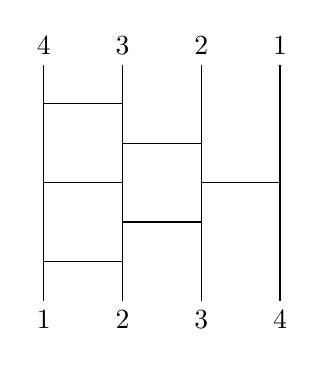
\begin{tikzpicture}
		 	\draw(0, 0) to (0, 3) ++(0, 0) node[above]{4} --(0, 0)node[below]{1};
		 		\draw(0, 2.5) to (1, 2.5);
		 		\draw(0, 1.5) to (1, 1.5);
		 		\draw(0, 0.5) to (1, 0.5);

		 	\draw(1, 0) to (1, 3) ++(0, 0) node[above]{3} --(1, 0)node[below]{2};
		 		\draw(1, 2) to (2, 2);
		 		\draw(1, 1) to (2, 1);
		 	\draw(2, 0) to (2, 3) ++(0, 0) node[above]{2} --(2, 0)node[below]{3};
		 		\draw(2, 1.5) to (3, 1.5);
		 	\draw(3, 0) to (3, 3) ++(0, 0) node[above]{1} --(3, 0) node[below]{4};
		\end{tikzpicture}
				

	\end{minipage}
	\begin{minipage}{.4\textwidth}
		\begin{flushright}
		
		
		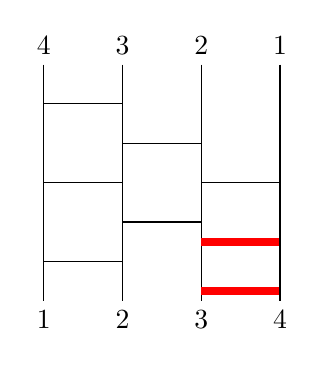
\begin{tikzpicture}
		 	\draw(0, 0) to (0, 3) ++(0, 0) node[above]{4} --(0, 0)node[below]{1};
		 		\draw(0, 2.5) to (1, 2.5);
		 		\draw(0, 1.5) to (1, 1.5);
		 		\draw(0, 0.5) to (1, 0.5);
		 		

		 	\draw(1, 0) to (1, 3) ++(0, 0) node[above]{3} --(1, 0)node[below]{2};
		 		\draw(1, 2) to (2, 2);
		 		\draw(1, 1) to (2, 1);
		 	\draw(2, 0) to (2, 3) ++(0, 0) node[above]{2} --(2, 0)node[below]{3};
		 		\draw(2, 1.5) to (3, 1.5);
		 		\draw[line width=1mm, red](2, 0.75) to (3, 0.75);
		 		\draw[line width=1mm, red](2, 0.125) to (3, 0.125);
		 	\draw(3, 0) to (3, 3) ++(0, 0) node[above]{1} --(3, 0) node[below]{4};
		\end{tikzpicture}
	\end{flushright}
	\end{minipage}
	\caption{Two ladders for the permutation (4, 3, 2, 1). The left ladder is an optimal ladder and the right ladder is not. Therefore the left ladder belongs to $optL\{(4,3,2,1)\}$. The bold  bars in the right ladder are redundant, thus the right ladder is not optimal}
	
\end{figure}


 


\chapter{Literature Review}
%%Intro to the Literature Review
\section{Introduction}
    The study of ladder lottieres as mathematical objects began in 2010, in  the paper
    \textbf{Efficient Enumeration of Ladder Lotteries and its Application}. The paper was 
    written by four authors, Yamanaka, Horiyama, Uno and Wasa. In this paper the 
    authors present an algorithm for generating all the ladder lotteries of an 
    arbitrary permutation, $\pi$. Since this paper emerged, there have been 
    several other papers written about ladder lotteries. 
    These papers include \textbf{The Ladder Lottery Realization Problem},
    \textbf{Optimal Reconfiguration of Optimal Ladder Lotteries}, 
    \textbf{Efficient Enumeration of all Ladder Lotteries with K Bars},
    \textbf{Coding Ladder Lotteries} and
    \textbf{Enumeration, Counting, and Random Generation of Ladder Lotteries}.

%$input review of first paper
\section{Efficient Enumeration of Ladder Lotteries and its Application}

%%Intro
In the Efficient Enumeration of Ladder Lotteries and its Application, written by Matsui, Nakada, Nakano Uehara and Yamanaka,
the authors provide an algorithm for generating $OptL\{\pi\}$ 
for any $\pi$, in $\mathcal{O}(1)$ per ladder~\cite{A1}. The authors refer to this algorithm as {\sc FindAllChildren}
which can be found in Algorithm~\ref{Alg:FindAllChildren}. 
\begin{algorithm}[!htp]
	\begin{algorithmic}[1]
		\Function{FindAllChildren}{$ladder$, $cleanLevel$, $n$}
			\State $currentRoute \gets n$
			\While{$currentRoute \geq cleanLevel$}
				\State going top left to bottom right 
				\For{$bar \in currentRoute$}
					\State $row \gets$ row of $bar$ in $ladder$ 
					\State $col \gets$ col of $bar$ in $ladder$
					\State $lowerNeighbor \gets ladder[row-1][col]$
					\If{$lowerNeighbor$ is right swappable}
						\State {\sc RightSwap($ladder$, $bar$, $lowerNeighbor$)}
						\State {\sc {\sc FindAllChildren}($ladder$, $y+1$, $n$)}
						\State {\sc LeftSwap($ladder$, $bar$, $lowerNeighbor$)}
					\EndIf
				\EndFor
				\State $currentRoute \gets currentRoute-1$
			\EndWhile
			\State $currentRoute \gets cleanLevel-1$
			\For{$bar \in currentRoute$}
				\State $row \gets$ row of $bar$ in $ladder$ 
				\State $col \gets$ col of $bar$ in $ladder$
				\State $lowerNeighbor \gets ladder[row-1][col]$
				\If{$lowerNeighbor$ is right swappable \textbf{and} is the rightmost bar of $currentRoute-1$}
					\State {\sc RightSwap($ladder$, $bar$)}
					\State {\sc FindAllChildren($ladder$, $cleanLevel$, $n$)}
					\State {\sc LeftSwap($ladder$, $bar$)}
				\EndIf
			\EndFor
		\EndFunction
	\end{algorithmic}
	\caption{The algorithm for listing $OptL\{\pi\}$.}
	\label{Alg:FindAllChildren}
\end{algorithm}
\pagebreak

One will note that two helper functions, {\sc RightSwap} and {\sc LeftSwap}, are required to complete 
{\sc FindAllChildren}. The details of these algorithms are not found 
in the paper~\cite{A1}. Thus, these algorithms and their details can be found in the Appendix in Algorithm \ref{Alg:RightSwap}
and Algorithm \ref{Alg:LeftSwap}.
{\sc FindAllChildren} is the first algorithm for generating $OptL\{\pi\}$.\newline
{\sc FindAllChildren} enumerates $OptL\{\pi\}$ as a tree of ladders.

%%Put this in the Appendix

%%DONE PUT IN Appendix

%%%%%%%%%%%%%%%%%%%%%%%%%%%%%%%FIND ALL CHILDREN ALGORITHM%%%%%%%%%%%%%%%%%%%%%%%%%%%%%



%%%%%%%%%%%%%%%%%%END ALGORITHM%%%%%%%%%%%%%%%%%%%%%%%%%%



{\sc FindAllChildren} was used in this thesis to generate the sample data that aided in finding solutions for 
the Gray Code Problem in Chapter 3 and the Minimum Height Problem in Chapter 4.  
Therefore, this algorithm is paramount for the findings of this thesis. 
To see the tree structure generated by {\sc FindAllChildren} for $OptL\{(4,3,2,1)\}$ 
please refer to Figure~\ref{Fig:TreeFAC}. 
\begin{figure}[h]
	\centering 
	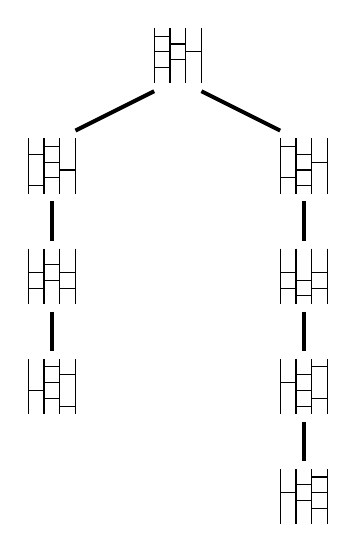
\begin{tikzpicture}
		%%L1
		\draw(5, 10) to (5, 9.3);
			\draw(5, 9.9) to (5.2, 9.9);
			\draw(5.2, 9.8) to (5.4, 9.8);
			\draw(5.4, 9.7) to (5.6, 9.7);
		\draw(5.2, 10) to (5.2, 9.3);
			\draw(5, 9.7) to (5.2, 9.7);
			\draw(5.2, 9.6) to (5.4, 9.6);
		\draw(5.4, 10) to (5.4, 9.3);
			\draw(5, 9.5) to (5.2, 9.5);
		\draw(5.6, 10) to (5.6, 9.3);
		%L2
		\draw[line width = .5mm](5, 9.2) to (4, 8.7);
		\draw[line width = .5mm](5.6, 9.2) to (6.6, 8.7);
			%%L2
			\draw(3.4, 8.6) to (3.4, 7.9);
				\draw(3.4, 8.4) to (3.6, 8.4);
				\draw(3.4, 8) to (3.6, 8);
			\draw(3.6, 8.6) to (3.6, 7.9);
				\draw(3.6, 8.5) to (3.8, 8.5);
				\draw(3.6, 8.3) to (3.8, 8.3);
				\draw(3.6, 8.1) to (3.8, 8.1);
			\draw(3.8, 8.6) to (3.8, 7.9);
				\draw(3.8, 8.2) to (4, 8.2);
			\draw(4.0, 8.6) to (4.0, 7.9);

				%%level
				\draw[line width = .5mm](3.7, 7.8) to (3.7, 7.3);
			\draw(3.4, 7.2) to (3.4, 6.5);
				\draw(3.4, 6.9) to (3.6, 6.9);
				\draw(3.4, 6.7) to (3.6, 6.7);
			\draw(3.6, 7.2) to (3.6, 6.5);
				\draw(3.6, 7) to (3.8, 7);
				\draw(3.6, 6.8) to (3.8, 6.8);
			\draw(3.8, 7.2) to (3.8, 6.5);
				\draw(3.8, 6.9) to (4, 6.9);
				\draw(3.8, 6.7) to (4, 6.7);
			\draw(4.0, 7.2) to (4.0, 6.5);

		%%L3
			\draw(6.6, 8.6) to (6.6, 7.9);
				\draw(6.6, 8.5) to (6.8, 8.5);
				\draw(6.8, 8.4) to (7, 8.4);
				\draw(7, 8.3) to (7.2, 8.3);
			\draw(6.8, 8.6) to (6.8, 7.9);
				\draw(6.8, 8.2) to (7, 8.2);
				\draw(6.8, 8) to (7, 8);
			\draw(7, 8.6) to (7, 7.9);
				\draw(6.6, 8.1) to (6.8, 8.1);
			\draw(7.2, 8.6) to (7.2, 7.9);
			
			
			\draw[line width = .5mm](6.9, 7.8) to (6.9, 7.3);

			\draw(6.6, 7.2) to (6.6, 6.5);
				\draw(6.6, 6.9) to (6.8, 6.9);
				\draw(6.6, 6.7) to (6.8, 6.7);
			\draw(6.8, 7.2) to (6.8, 6.5);
				\draw(6.8, 6.8) to (7, 6.8);
				\draw(6.8, 6.6) to (7, 6.6);
			\draw(7.0, 7.2) to (7.0, 6.5);
				\draw(7, 6.9) to (7.2, 6.9);
				\draw(7, 6.7) to (7.2, 6.7);
			\draw(7.2, 7.2) to (7.2, 6.5);

			\draw[line width = .5mm](3.7, 6.4) to (3.7, 5.9);

			\draw(3.4, 5.8) to (3.4, 5.1);
				\draw(3.4, 5.4) to (3.6, 5.4);
			\draw(3.6, 5.8) to (3.6, 5.1);
				\draw(3.6, 5.7) to (3.8, 5.7);

				\draw(3.6, 5.5) to (3.8, 5.5);
				\draw(3.6, 5.3) to (3.8, 5.3);
			\draw(3.8, 5.8) to (3.8, 5.1);
				\draw(3.8, 5.6) to (4, 5.6);
				\draw(3.8, 5.2) to (4, 5.2);
			\draw(4.0, 5.8) to (4.0, 5.1);

			\draw[line width = .5mm](6.9, 6.4) to (6.9, 5.9);

			
			\draw(6.6, 5.8) to (6.6, 5.1);
				\draw(6.6, 5.5) to (6.8, 5.5);
			\draw(6.8, 5.8) to (6.8, 5.1);
				\draw(6.8, 5.6) to (7, 5.6);

				\draw(6.8, 5.4) to (7, 5.4);
				\draw(6.8, 5.2) to (7, 5.2);
			\draw(7.0, 5.8) to (7.0, 5.1);
				\draw(7.0, 5.7) to (7.2, 5.7);
				\draw(7.0, 5.3) to (7.2, 5.3);
			\draw(7.2, 5.8) to (7.2, 5.1);

			\draw[line width = .5mm](6.9, 5) to (6.9, 4.5);

			\draw(6.6, 4.4) to (6.6, 3.7);
				\draw(6.6, 4.1) to (6.8, 4.1);
			\draw(6.8, 4.4) to (6.8, 3.7);
				\draw(6.8, 4.2) to (7, 4.2);

				\draw(6.8, 4) to (7, 4);
			\draw(7.0, 4.4) to (7.0, 3.7);
				\draw(7.0, 4.3) to (7.2, 4.3);
				\draw(7.0, 4.1) to (7.2, 4.1);
				\draw(7.0, 3.9) to (7.2, 3.9);
			\draw(7.2, 4.4) to (7.2, 3.7);



	\end{tikzpicture}
	\caption{The tree structure of $OptL\{(4,3,2,1)\}$ generated by {\sc FindAllChildren}}
	\label{Fig:TreeFAC}
\end{figure}
\pagebreak
{\sc FindAllChildren} is based on several key concepts. One of which is the local swap operation 
which has already been discussed. The next fundamental concept is the \emph{route} of an element, 
which is the sequence of bars the element travels along in order to reach its final position in the 
sorted permutation. The bars are read from top to bottom. For every bar, two elements cross 
the bar, therefore the bar is associated with the route of the greater of the two elements~\cite{A1}. 
In Figure~\ref{Fig:Route} the route of element $4$ is the sequence of bars 
$(4,1),(4,2),(5,4)$. To see the route of an element please refer to Figure~\ref{Fig:Route}. When a 
right swap operation occurs, the bar of the route associated with a lesser element is 
swapped above two bars of a route associated with a greater element. For example, in Figure~\ref{fig:rightSwap} in the right ladder, 
the bar $(3,1)$ which is associated with the route of element $3$ is right swapped above the two bars $(5,1)$ and $(5,3)$ 
both of which are associated with the route of $5$.\par 
\begin{figure}[h]
	\centering
	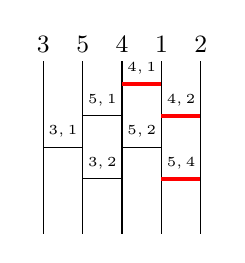
\begin{tikzpicture}
		\draw(0, 0) to (0, 2.2);
			\node at(.25, 1.3){\tiny{$3,1$}};
			\draw(0, 1.1) to (.5, 1.1);
		\draw(.5, 0) to (.5, 2.2);
			\node at(.75, 1.7){\tiny{$5,1$}};
			\draw(.5, 1.5) to (1, 1.5);
			\node at(.75, .9){\tiny{$3,2$}};
			\draw(.5, .7) to (1, .7);
		\draw(1, 0) to (1, 2.2);
			\node at(1.25, 2.1){\tiny{$4,1$}};
			\draw[line width=.5mm, red ](1, 1.9) to (1.5, 1.9);
			\node at(1.25, 1.3){\tiny{$5,2$}};
			\draw(1, 1.1) to(1.5, 1.1);
		\draw(1.5, 0) to (1.5, 2.2);
			\node at(1.75, 1.7){\tiny{$4,2$}};
			\draw[line width=.5mm, red ](1.5, 1.5) to (2, 1.5);
			\node at(1.75, .9){\tiny{$5,4$}};
			\draw[line width=.5mm, red ](1.5, .7) to (2, .7);
		\draw(2, 0) to (2, 2.2);


		\node at(0.0, 2.4){\small{$3$}};
		\node at(0.5, 2.4){\small{$5$}};
		\node at(1.0, 2.4){\small{$4$}};
		\node at(1.5, 2.4){\small{$1$}};
		\node at(2.0, 2.4){\small{$2$}};
	\end{tikzpicture}
	\caption{The route of element 4=(4,1),(4,2),(5,4).}
	\label{Fig:Route}
\end{figure}



The \emph{clean level} is defined as one more than the largest 
element associated with any bar that has undergone a right swap operation. 
For example, if the largest element associated with a bar that has undergone a 
right swap operation is element $4$, then the clean level is $5=4+1$.
 Please refer to Figure~\ref{Fig:CleanLevel} for an example of the clean level.
 If no bars have been right swapped, then the clean level is $1$.
If the largest element to have undergone a right swap operation is the maximal element in $\pi$, 
then the clean level is $max+1$.\pagebreak

\begin{figure}[t]
	\centering 
	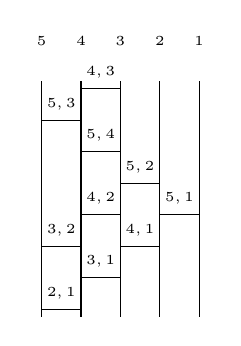
\begin{tikzpicture}
		\draw(0, 0) to (0, 3);
			\node at(.25, 2.7){\tiny{$5,3$}};
			\node at(.25, 1.1){\tiny{$3,2$}};
			\node at(.25, .3){\tiny{$2,1$}};
			\draw(0, 2.5) to (.5, 2.5);			
			\draw(0, .9) to (.5, .9);
			\draw(0, .1) to (.5, .1);

		\draw(.5, 0) to (.5, 3);
			\node at(.75, 3.1){\tiny{$4,3$}};
			\node at(.75, 2.3){\tiny{$5,4$}};
			\node at(.75, 1.5){\tiny{$4,2$}};
			\node at(.75, .7){\tiny{$3,1$}};

			\draw(.5, 2.9) to (1, 2.9);
			\draw(.5, 2.1) to (1, 2.1);
			\draw(.5, 1.3) to (1, 1.3);
			\draw(.5, .5) to (1, .5);
		\draw(1, 0) to (1, 3);
			\node at(1.25, 1.9){\tiny{$5,2$}};
			\node at(1.25, 1.1){\tiny{$4,1$}};

			\draw(1, 1.7) to (1.5, 1.7);
			\draw(1, .9) to (1.5, .9);
		\draw(1.5, 0) to (1.5, 3);
			\node at(1.75, 1.5){\tiny{$5,1$}};
			\draw(1.5, 1.3) to (2, 1.3);
		\draw(2, 0) to (2, 3);

		%%%%%%%%%%%%%%%%%%%%%%%%%%%%
		\node at(0, 3.5){\tiny{$5$}};
		\node at(.5, 3.5){\tiny{$4$}};
		\node at(1, 3.5){\tiny{$3$}};
		\node at(1.5, 3.5){\tiny{$2$}};
		\node at(2, 3.5){\tiny{$1$}};
\end{tikzpicture}
	\caption{A ladder with a clean level of $6$. The largest element whose associated bars have undergone a right swap operation is $5$}
	\label{Fig:CleanLevel}
\end{figure}


Each $OptL\{\pi\}$ has a unique ladder with a clean level of one. This ladder 
is known as the \emph{root ladder}. The root ladder is the root of the tree structure 
produced from {\sc FindAllChildren}. Unlike every other ladder in the tree, 
the root ladder cannot be derived from a local swap operation. Thus, the root ladder 
must be created by another algorithm other than {\sc FindAllChildren}. 
The authors do not provide details on how to create the root ladder. Thus, an 
algorithm for creating the root ladder can be found in the Appendix in Algorithm~\ref{Alg:RootLadder}.
The details of the root ladder are also explained in the Appendix.
Given all permutations of order $n$, the root ladder for the descending permutation requires 
the most rows. 
\begin{theorem}
  The number of rows required for the root ladder of the descending permutation is $2(n-1) - 1$.
\end{theorem}
\begin{proof}
  The number of rows for the ladder data-structure is calculated a follows: When a bar is added to the ladder it can be added 
  to an already existing row or to a new row. 
  If the current state of the ladder is empty then adding the first bar produces the second ladder in
  $L_{n}$. Since the bars are being added bottom right to top left, and the first bar to be added belongs 
  to the $nth$ route, then it must be added to $row=n-1$, $col=n-1$. As bars of the $nth$ route get 
  continuously added to the ladder, each bar is added a row above the previous bar and to a column 
  to the left of the column of the previous bar.
  Since no two bars of the $nth$ route can be on the same row, this will require $n-1$ rows. Note, if they were added to the same 
  row, then the left end point of the right bar would be touching the right end point of the left bar which is disallowed. Once the 
  bars of the $nth$ element are added, the bars of the $n-1th$ route will be added. The $n-1th's$ first bar 
  will be added to the $n-2$ column, otherwise it would be directly below the first bar of the $nth$ route, which is a violation. 
  Since the first bar of the $n-1$'s element is added to column $n-2$, then it must be given a new row, otherwise its right end point 
  will be touching  the left end point of the first bar of route $n$. The remaining $n-2$ bars of element $n-1$
  will be added bottom right to top left, but none of their end points will touch the end points of element $n$ seeing as they will 
  always be two columns apart from any bar in $n's$ route. The same logic applies to element $n-2$, it will require one extra row for its 
  first bar, in order not to touch the first bar of element $n-1$, but the remainder of its bars will always be two columns away from 
  the remainder of the bars for $n-1$, etc. Therefore there are $n-1$ rows required for the $nth$ element and each subsequent 
  element, $k$ requires only one new row. Since $2 \leq k < n$, then there are $(n-2)$ additional rows required for the ladder. Note that element 
  $1$ has no bars in its route. Therefore there are $(n-1)$ rows required for element $n's$ bars  plus $(n-2)$ rows required for 
  all the remaining $2 \leq k < n$ routes. In conclusion the number of rows required is $(n-1) + (n-2) = 2(n-1)-1$. 
  See figure for the tree of ladders 
  generated by {\sc ModifiedSJT} for $n=4$. Note that the maximum number of rows required is $2(n-1)-1=2(3)-1=5$.
\end{proof}



%%Root ladder subsection




%%DONE Appendix SECTION

In concluding the section on the enumeration problem, we have analyzed the original paper along with 
making additions to the algorithm {\sc FindAllChildren} by providing four essential algorithms 
for the completion of {\sc FindAllChildren}. The algorithms are Algorithm~\ref{Alg:RootLadder}, Algorithm~\ref{Alg:RightSwap},
Algorithm~\ref{Alg:LeftSwap} and Algorithm~\ref{Alg:ShiftSubLadder} which can be found in the Appendix. In concert, these five algorithms solve the enumeration 
problem which lists $OptL\{\pi\}$ in $O(1)$ time per ladder. 


\pagebreak

%%input revoiew of second paper


\subsection{Ladder-Lottery Realization}

In their paper \textbf{Ladder-Lottery Realization} the authors provide 
a rather interesting puzzle in regards to ladder lotteries. The puzzle 
is known as the ladder-lottery realization problem. In order to understand
the problem, one must know what a \emph{multi-set} is. A \emph{multi-set}
is a set in which an element appears more than once. The exponent 
above the element indicates the number of times it appears in the set.
For example, given the following multi-set, $\{3^{2}, 2^{4}, 5^{1}\}$ 
the element $3$ appears twice in the set, the element $2$ appears four times
in the set and the element $5$ appears once in the set.
The ladder-lottery realization puzzle asks, given an arbitrary starting permutation 
and a multi-set of bars, 
is there a \emph{non-optimal} ladder lottery for the arbitrary permutation
that uses every bar in the multi-set the number 
of times it appears in the  multi-set. 
For an example of an affirmative solution to the ladder lottery realization problem, see Fig. 2.4.


\begin{figure}[!htp]
    \begin{center}
        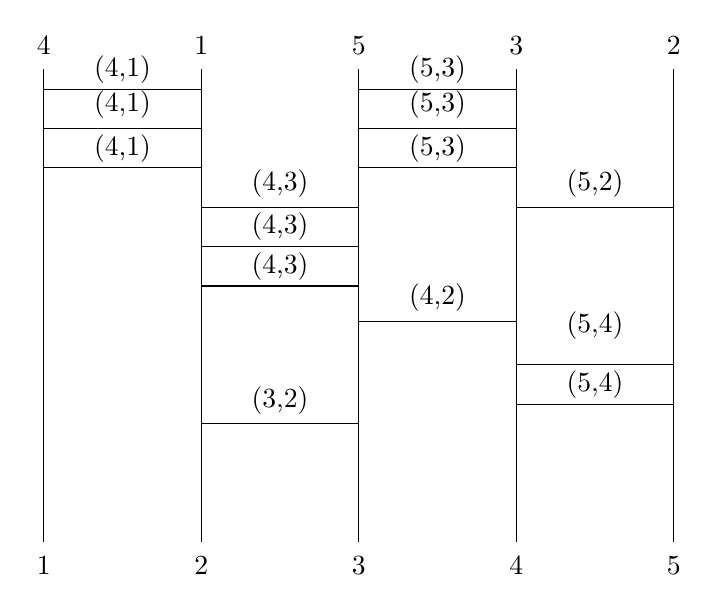
\begin{tikzpicture}
            \draw (0, 0) to (0, 6);
                \node at(0, -0.3){1};
                \node at(0, 6.3){4};
            \draw(2, 0) to (2, 6);
                \node at(2, -0.3){2};
                \node at(2, 6.3){1};
            \draw(4, 0) to (4, 6);
                \node at(4, 6.3){5};
                \node at(4, -0.3){3};
            \draw(6, 0) to (6, 6);
                \node at(6, 6.3){3};
                \node at(6, -0.3){4};
            \draw(8, 0) to (8, 6);
                \node at(8, 6.3){2};
                \node at(8, -0.3){5};

            %%draw the bars
                \node at(1, 6){(4,1)};
                    \draw(0, 5.75) to (2, 5.75);
            \draw(0, 5.25) to (2, 5.25);
                \node at(1, 5.55){(4,1)};
            \draw(0, 4.75) to (2, 4.75);
                \node at(1, 5){(4,1)};

            \draw(4, 5.75) to (6, 5.75);
                \node at(5, 6){(5,3)};
            \draw(4, 5.25) to (6, 5.25);
                \node at(5, 5.55){(5,3)};
            \draw(4, 4.75) to (6, 4.75);
                \node at(5, 5){(5,3)};

            \draw(2, 4.25) to (4, 4.25);
                \node at (3, 4.55){(4,3)};
            \draw(2, 3.75) to (4, 3.75);
                \node at (3, 4){(4,3)};
            \draw(2, 3.25) to (4, 3.25);
                \node at (3, 3.5){(4,3)};
            
            \draw(2, 1.5) to (4, 1.5);
                \node at(3, 1.8){(3,2)};
            
            \draw(4, 2.8) to (6, 2.8);
                \node at (5, 3.1){(4,2)};
            \draw(6, 4.25) to (8, 4.25);
                \node at (7, 4.55){(5,2)};
            
            \draw(6, 2.25) to (8, 2.25);
                \node at (7,2.75){(5,4)};
            
            \draw(6, 1.75) to (8, 1.75);
                \node at (7, 2){(5,4)};
            
        \end{tikzpicture}
    \end{center}
      


    \caption{An affirmative solution to the Ladder Lottery Realization Problem given a starting perumtation $(4,1,5,3,2)$ and the multi set of bars $\{(4,1)^{3}, (4,3)^{3}, (4,2)^{1}, (5,4)^{2}, (5,3)^{3}, (5,2)^{1},(3,2)^{1}\}$}
\end{figure}
\pagebreak
The authors prove that the ladder-lottery realization problem in NP-Hard
by reducing the ladder-lottery realization to the One-In-Three 3SAT, 
which has already been proven to be NP-Hard. The One-In-Three 3SAT 
problem is a problem such that given a set of variables $(X)$, a collection 
of \emph{disjuntcive clauses} $(C)$ which are disjunctive expressions over 
literals of $X$. Each clause in $C$ 
must contain three literals then is there a truth assignment for $X$ such that 
each clause in $C$ has exactly one true literal. For eaxmple, let 
$X=\{p, q, r, s, t\}$ and let $C=\{C_{p,q,s}, C_{r,q,s} C_{p,s,t}, C_{r,t,q}\}$,
the question is whether it is possible for each clause to have exactly one
true literal. The answer in this case is yes. If $p=T$, $r=T$, $q=F$, $s=F$
 and $t=T$ then all the clauses in $C$ have exactly one true literal. 
 The authors reduce the ladder lottery-realization problem to the
One-In-Three 3SAT problem by devising four gadgets. The result of 
the reduction is that the arbitrary starting permutation is equivelent 
to a derivation of the intial set of variables, $X$, in the One-In-Three 3SAT 
problem and the multi-set of bars is equivelent to a 
derivation of the intial set of clauses, $C$, in the One-In-Three 
3SAT problem.\par 
The authors note that there are two cases in which the ladder-lottery
realization problem can be solved in polynomial time. These cases 
include the follwing. First, if every bar in the multi-set appears
exactly once and every bar corresponds to an inversion, 
then an affirmative solution to the ladder-lottery realization 
instance can be demonstrated in polynomial time. 
Second, if there is an inversion in the perumutation and its bar appears in the multi-set an even 
number of times, then a negative solution to
the ladder-lottery realization instance
can be solved in polynomial time.\par

%%input review of third paper

\section{Optimal Reconfiguration of Optimal Ladder Lotteries}
A local swap operation, corresponding to a braid relation in algebra, is a local modification of a ladder lottery 
demonstrated in Figure~\ref{Fig:LocalSwap}~\cite{A1}.
\begin{figure}[h]
    \centering 
    \resizebox{!}{.3\textheight}{
            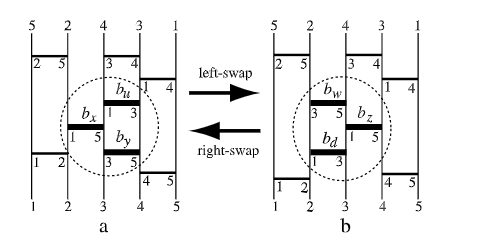
\includegraphics{LocalSwapOperation}
    }
    \caption{A local swap operation}
    \label{Fig:LocalSwap}
\end{figure}

In \emph{Optimal Reconfiguration of Optimal Ladder Lotteries}~\cite{A2}, written by Horiyama, Wasa and Yamanaka,
the authors provide a polynomial solution to the 
Minimal Reconfiguration Problem which asks, given 
two ladders, $L_{i}$ and  $L_{m}$, what is the minimal number of 
swap operations to perform that will transition from $L_{i}$ to $L_{m}$? A \emph{reverse triple} 
is a relation between three bars, $x,y,z$ in two arbitrary ladders, $L_{i}, L_{m}$, such that if $x,y,x$
are right swapped in $L_{i}$, then they are left swapped in $L_{m}$ or if they are 
left swapped in $L_{i}$ then they are right swapped in $L_{m}$. 
Let an \emph{improving triple} be defined as  
performing a right/left swapping three bars, $x,y,z$, in $L_{i}$ such that the 
result of the swap removes a reverse triple between
ladders $L_{i}$ and $L_{m}$. The improving triple is a symmetric 
relation, therefore performing a right/left swapping of the $x,y,z$ in $L_{m}$ also results in the 
removal of a reverse triple between $L_{i}$ and $L_{m}$.\par
The \emph{minimal length reconfiguration sequence} is the minimal number of 
improving triples required to transition from $L_{i}$ to $L_{m}$ or 
$L_{m}$ to $L_{i}$. Transitioning from $L_{i}$ to $L_{m}$ with the minimal length reconfiguration sequence 
is achieved by applying an improving triple to each of the reverse triples between 
$L_{i}$ and $L_{m}$. That is to say, the length of the reconfiguration sequence 
is equal to the number of improving triples required to remove all reverse triples between $L_{i}$ and  $L_{m}$.\par
The second contribution of this paper is that it provides a closed form formula for the 
upper bound for the minimal length reconfiguration sequence for any permutation 
of size $n$. That is to say, given some arbitrary $\pi$ of order $n$, what is the maximum 
number of swaps required for the minimal length reconfiguration sequence between any two ladders in $OptL\{\pi\}$?
The authors prove that there are two unique ladders in $OptL\{(n, n-1, \dots, 1)\}$ that 
have the upper bound for the minimal length reconfiguration sequence. These ladders are the root ladder and \emph{final ladder} 
which is defined as the unique ladder in $OptL\{\pi\}$ such that $\forall z < y < x: (y,z) \text{ is above } (x,z) \in l$. 
The length of the reconfiguration sequence 
between the root ladder and final ladder in $OptL\{(n, n-1, \dots, 1)\}$ is $n{n-1~\choose 2}$. 
\par

%%input review of fourth paper.

\subsection{Efficient Enumeration of all Ladder Lotteries with K Bars}

In this paper, the authors apply the same algorithm used in Efficient Enumeration of Optimal Ladder-Lotteries 
and its Application for generating all ladder lotteries with k bars \cite{A4}. The number of elements 
in The inversion set of $\pi$ also known as $Inv\{\pi\}$ provides the lower bound for $K$ 
and the upper bound is positive infinity. Therefore $K=[|Inv\{\pi\}| \dots N]$ \cite{A4}.\par\par 
\subsection{Coding Latter Lotteries}
\subsubsection{Overview}
In this paper, the authors provide three methods to encode ladder-lotteries as 
binary strings. Coding discrete objects as binary strings is an appealing theme because 
it allows for compact represntation of them for a computer \cite{A5}.
\subsubsection{Route Based Encoding}
The first method is termed \emph{route based encoding method} in 
which each route of an element in the permutation has a binary encoding. Let $L$
be a ladder-lottery for some arbitrary permutation $\pi$ of order $N$. The route 
of element $p_{i}$ is encoded by keeping in mind $p_{i}$ crosses bars in its route 
going left zero or more times and crosses bars in its route going right zero or 
more times \cite{A5}. The maximum number of bars $p_{i}$ can have is $N-1$, therefore the 
upper bound for the number of left/right crossings for $p_{i}$ is $N-1$ \cite{A5}. 
Let a left crossing be denoted with a $'0'$ and let a right crossing be denoted 
with a $'1'$. Let $C_{p_{i}}$ be the route encoding for the $i^{th}$ element 
in $\pi$. To construct $C_{p_{i}}$,  append $0$ and $1$ to each other representing 
the left and right crossings of $p_{i}$ from the top left 
to bottom right of the ladder \cite{A5}. If the number of crossings for $p_{i}$ 
is less than $n-1$, append $0s$ to the encoding of the route of $p_{i}$ until
the encoding is of length $N-1$ \cite{A5}. Let $LC_{L}$ be the route encoding for 
some arbitrary ladder in $OptL\{\pi\}$. $LC_{L}$ is $C_{p_{1}}, C_{p_{2}, \dots C_{p_{N}}}$.
For an example of the route encoding for the root ladder of $(3,2,5,4,1)$ refer to 
Fig.\ref{fig:route-encoding}. In \ref{fig:route-encoding}you will see that $C_{p_{1}}$ is 11\underline{00}. Underlined 
$0s$ are the $0s$ added to ensure the length of $C_{p_{1}}$ is $N-1$.
Since the length of $C_{pi}$ is $N-1$ and the number of elements in $\pi$ is $N$
then the length of $LC_{L}=N(N-1)$. Hence the number of bits needed for $LC_{L}$ 
belongs to $\mathcal{O}(N^{2})$.\par 
\begin{figure}[!htp]
    \begin{center}
        \begin{tikzpicture}
    
            %%draw the lines
            \draw(0, 0) to (0, 4);
                \node at(0, 4.3){3};
                \node at(0, -0.3){1};
            \draw(2, 0) to (2, 4);
                \node at (2, 4.3){2};
                \node at(2, -0.3){2};
            \draw(4, 0) to (4, 4);
                \node at (4, 4.3){5};
                \node at (4, -0.3){3};
            \draw(6, 0) to (6, 4);
                \node at (6, 4.3){4};
                \node at (6, -0.3){4};
            \draw(8, 0) to (8, 4);
                \node at (8, 4.3){1};
                \node at (8, -0.3){5};
    
            %%Draw the bars
            \draw(0, 2) to (2, 2);
            \draw(2, 1.5) to (4,1.5);
            \draw(0, 1) to (2, 1);

            \draw(4, 3) to (6, 3);
            \draw(6, 2.5) to (8, 2.5);
            \draw(4, 2) to (6, 2);
        \end{tikzpicture}
    \end{center}
   
 \caption{The route encoding for the following ladder lottery is 11\underline{00}01\underline{00}11\underline{00}01\underline{00}0000}
 \label{fig:route-encoding}

\end{figure}

\subsubsection{Line Based Encoding}
The second method is termed \emph{line based encoding} which focuses 
on encoding the lines of the ladder-lottery. Each line is represented 
as a sequence of endpoints of bars. Let $L$ be an optimal ladder-lottery 
with $N$ lines and $B$ bars, then for some arbitrary line, $i$, there 
are zero or more right/left endpoints of bars that 
come into contact with $i$ \cite{A5}. Let $LC_{i}$ denote the line based encoding for line $i$.
Let $1$ denote a left end point that 
comes into contact with line $i$ and let $0$ denote a right 
end point that comes into contact with line $i$. Finally, append a $0$
to line $i$ to denote the end of the line. Then line $i$ can be 
encoded, from top to bottom, as a sequence of $1s$ and $0s$ that 
terminates in a $0$.  Given the ladder in Fig. \ref{fig:line-encoding}, 
$LC_{3}$ is $001\underline{0}$. The \underline{0} denotes 
the end of the line. Let $LC_{L}$ be the line encoding for 
some arbitrary ladder, then $LC_{L}=LC_{1}, LC_{2}, \dots LC_{N}$.
Let $L_{(4,2,3,1)}$ refer to the ladder in Fig. \ref{fig:line-encoding}, then 
$LC_{L_{(4,2,3,1)}}=11\underline{0}010\underline{0}110\underline{0}010\underline{0}0\underline{0}$\par 
In order to reconstruct $L$ from its $LC_{L}$, or in other words decode
$LC_{L}$ it is important to recognize that the first line only has left endpoints attached to it
\cite{A5}. Since left end points are encoded as a $1$ then it is guarenteed that the first $0$ 
represents the end of line $1$. Secondly, the last/$Nth$ line 
has only right end points attached to it.  Therefore $LC_{N}$ will only have $0s$. Therefore, $LC_{N}$
does not require a terminating $0$. Thirdly, for any 
line $i+1$, if line $i+1$ has a $0$ then there must be a corresponding $1$
in line $i$. That is to say, if the right end point of a bar is on line 
$i+1$ then that same bar must have a left endpoint on line $i$. To decode 
$LC_{L}$ start by decoding line $1$. The line will contain $0$ or more 
left end points. To decode $LC_{i+1}$ where $i+1>1$, go to 
$LC_{i}$ and match each $1$ in $LC_{i}$ with a $0$ in $LC_{i+1}$. 
Let $k=$ the number of $1s$ in $LC_{i}$. Let $j=$ the number 
of $0s$ in $LC_{i+1}$ then $k=j-1$; due to the last $0$ in $LC_{i+1}$ denoting 
the end of line $i+1$.  Intuitively, this means match every left end point 
of a bar in line $i$ with a right end point in line $i+1$. The last $0$
represents the end of line $i+1$. For an example of a full decoding of $LC_{L_{(4,2,3,1)}}$
please refer to Fig. \ref{fig:line-encoding}.\pagebreak
\begin{figure}[!htp]
    \begin{center}
        \begin{tikzpicture}
            \draw(0, 0) to (0, 4);
            \node at (0, 4.3){4};
            \node at (0, -0.3){1};
        \draw(2, 0) to (2, 4);
            \node at (2, 4.3){2};
            \node at (2, -0.3){2};
        \draw(4, 0) to (4, 4);
            \node at (4, 4.3){3};
            \node at (4, -0.3){3};
        \draw(6, 0) to (6, 4);
            \node at (6, 4.3){1};
            \node at (6, -0.3){4};

        %%bars 
        \draw(0, 3) to (0.7, 3);
            \node at (0.35, 3.3){1};
        \draw (1.3, 3) to (2, 3);
            \node at (1.65, 3.3){0};

        \draw(2, 2.5) to (2.7, 2.5);
            \node at (2.35, 2.8){1};
        \draw(3.3, 2.5) to (4, 2.5);
            \node at (3.65, 2.8){0};

        \draw(4, 2) to (4.7, 2);
            \node at (4.35, 2.3){1};
        \draw(5.3, 2) to (6, 2);
            \node at (5.65, 2.3){0};

      

        \draw(2, 1) to (2.7, 1);
            \node at (2.35, 1.3){1};
        \draw(3.3, 1) to (4, 1);
            \node at (3.65, 1.3){0};

        \draw(0, 0.5) to (0.7, 0.5);
            \node at (0.35, 0.8){1};
        \draw(1.3, 0.5) to (2, 0.5);
            \node at (1.65, 0.8){0};

        \end{tikzpicture}
      

    \end{center}
    \caption{$LC_{L(4,2,3,1)}=LC_{1}=11\underline{0},LC_{2}=0110\underline{0},LC_{3}=010\underline{0},LC_{4}=0$}
    \label{fig:line-encoding}
\end{figure}

Since each bar is encoded as two bits, and there are $N-1$ bits as terminating bits; 
one for each line in $L$, then the number of bits required is $N + 2B -1$, where $N$
is the number of lines and $B$ is the number of bars. Encoding and decoding can be 
done in $\mathcal{O}(n+b)$ time.\cite{A5} Clearly the line-based encoding 
trumps the route-based encoding in both time and space complexity.

\subsubsection{Improved Line-Based Encoding}
Although the line-based encoding is better than the route based 
encoding, it can still be further optimized. The authors provide 
three improvements to the line-based encoding. These three improvements
can be combined to really help imrpove the line based encoding's 
space efficiency \cite{A5}. 
\paragraph{Imrpovement 1}
Since the $Nth$ line has only right endpoints attached to it, 
then it actually does not need to be encoded. Right endpoints 
are denoted as $0$ and left endpoints are encoded as $1$, therefore the number of right endpoints 
for line $N$ is equal to the number of $1s$ in $LC_{N-1}$.
Thus, there is no need for $LC_{N}$ \cite{A5}. The encoding with improvment 
one for the ladder in Fig. \ref{fig:line-encoding} is $11\underline{0}0110\underline{0}010$.
\paragraph{Improvement 2}
Improvement two is based off of the fact that for any two bars,
$x,y$, let $l_{x}$ denote the left endpoint of bar $x$, let 
$l_{y}$ denote the left endoint of bar $y$, let $r_{x}$ denote 
the right end point of bar $x$ and let $r_{y}$ denote the right 
end point of bar $y$. Let line $i$ be the line of $l_{x}$ and $l_{y}$
and let line $i+1$ be the line of $r_{x}$ and $r_{y}$.
\begin{lemma}
There are three possible cases for the 
placement of $x$ and $y$ in some 
arbitrary ladder from $OptL\{\pi\}$. The first case is that there 
is at least one other bar, $z$, with a right end point, $r_{z}$ between $l_{x}$
and $l_{y}$ on line $i$. The second case is that there is at least one other bar 
$z$, with a left end point, $l_{z}$, between $r_{x}$ and $r_{y}$ on line $i+1$. 
The third case is that there is at least one bar, $z$, with a right end point, 
$r_{z}$, betwen $l_{x}$ and $l_{y}$ on line $i$ and there is at least one other bar, 
$z\prime$ with a left end point, $l_{z\prime}$, between $r_{x}$ and $r_{y}$ on line $i+1$ \cite{A5}. 
For an example of all three cases refer to Fig. \ref{fig:three-cases}\par
\end{lemma}

%%figure demonstrating the three cases for bar positions
\begin{figure}[!htp]
       
            %%first case
            \begin{minipage}{.3\textwidth}
                \begin{tikzpicture}
                    \draw(0, 0) to (0, 4);
                        \node at (2, 4.3){\small{$i+1$}};
                    \draw(1, 0) to (1, 4);
                        \node at (1, 4.3){\small{$i$}};
                    \draw(2, 0) to (2, 4);
                        \node at (0, 4.3){\small{$i-1$}};
                    \draw(0, 2) to (1, 2);
                        \node at (.5, 2.3){\small{$r_{z}$}};
                    \draw(1, 3) to (2, 3);
                        \node at (1.5, 3.3){\small{$l_{x}$}};
                    \draw(1, 1) to (2, 1);
                        \node at (1.5, 1.3){\small{$l_{y}$}};
                \end{tikzpicture}
            \end{minipage}
              \begin{minipage}{.3\textwidth}

                 \begin{tikzpicture}
                
                  \draw(0, 0) to (0, 4);
                     \node at (0, 4.3){\small{$i-1$}};
                  \draw(1, 0) to (1, 4);
                    \node at (1, 4.3){\small{$i$}};
                  \draw(2, 0) to (2, 4);
                     \node at (2, 4.3){\small{$i+1$}};
                   \draw(0, 3) to (1, 3);
                         \node at (.5, 3.3){\small{$r_{x}$}};
                    \draw(1, 2) to (2, 2);
                         \node at (1.5, 2.3){\small{$l_{z}$}};
                     \draw(0, 1) to (1, 1);
                         \node at (0.5, 1.3){\small{$r_{y}$}};
                
                   
                
                \end{tikzpicture}
             \end{minipage}
             \begin{minipage}{.3\textwidth}

                \begin{tikzpicture}
                
                 \draw(0, 0) to (0, 4);
                    \node at (1, 4.3){\small{$i$}};
                 \draw(1, 0) to (1, 4);
                    \node at (2, 4.3){\small{$i+1$}};
                 \draw(2, 0) to (2, 4);
                    \node at (0, 4.3){\small{$i-1$}};
                 \draw(3, 0) to (3, 4);
                    \node at (3, 4.3){\small{$i+2$}};
                    \draw(1, 3) to (2, 3);
                        \node at (1.3, 3.3){\small{$l_{x}$}};
                        \node at (1.7, 3.3){\small{$r_{x}$}};
                     \draw(0, 2) to (1, 2);
                        \node at (0.7, 2.3){\small{$r_{z}$}};
                    \draw(1, 1) to (2, 1);
                        \node at (1.3, 1.3){\small{$l_{y}$}};
                         \node at (1.7, 1.3){\small{$r_{y}$}};
                     \draw(2, 2) to (3, 2);
                        \node at (2.3, 2.3){\small{$l_{z\prime}$}};
                
                   
                
                \end{tikzpicture}
            \end{minipage}
        

    \caption{Three examples of the three cases for the placement 
    of bars $x$ and $y$ in a ladder-lottery}
    \label{fig:three-cases}
\end{figure}
\begin{proof}
    Suppose that none of the above cases hold. Let $L_{\pi}$ be an 
    optimal ladder-lottery with bars $x$ and 
    bar $y$. If none of the cases hold then $x$ and $y$ are directly above/below each other without 
    the enpoint of some third bar $z$ between $l_{x}$ and $l_{y}$ or between $r_{x}$ and $r_{y}$.
    Let $x$ be the bar for the inversion of two elements $p$ and $q$ in $\pi$. 
    As $p$ and $q$ travel through the ladder they will cross each other at bar $x$; 
    thus uninverting them. Since bar $y$ is directly below bar $x$, then $p$ and $q$ will cross 
    bar $y$ thus re-inverting them. Therefore, there will need to be a third 
    bar that uninverts $p$ and $q$ a second time. Since this third bar is 
    redundant, $L_{\pi}$ is non-optimal which is a contradiction. Let $x$ be a bar for two 
    elements in $\pi$, $p$ and $q$ such that $p$ and $q$ do not form an inversion. Then $x$ 
    will invert $p$ and $q$ and $y$ will uninvert them. Thus making both $x$ and $y$ redundant
    bars which is also a contradiction. Therefore one of the above cases must hold.
\end{proof}
Knowing that one of the three above cases must hold is beneficial for improving the 
line-based encoding. If $l_{x}$ and $l_{y}$ on line $i$ have no $r_{z}$ between them, 
then there must be at least one $l_{z\prime}$ between $r_{x}$ and $r_{y}$ on line $i+1$.
Since a left endpoint is encoded as a $1$ and a right endpoint is encoded as a $0$, 
a $1$ can be omitted for the encoding of line $i+1$ if $l_{x}$ and $l_{y}$ have no $r_{z}$
between them on line $i$ \cite{A5}. That is to say, if there is not a $0$ between 
the two  $1s$ for $l_{x}$, $l_{y}$ in $LC_{i}$, it is implied that there is at least one $1$ between 
the two $0s$ for $r_{x}$, $r_{y}$ on $LC_{i+1}$. Hence, one of the $1s$ in $LC_{i+1}$ can be omitted. 
The line encoding with improvement two for the ladder in Fig. \ref{fig:line-encoding} is $11\underline{0}010\underline{0}00\underline{0}0$.
\paragraph{Imrpovement 3}
Improvement three is based off of saving some bits for right 
end points/$0s$ in $LC_{N-1}$. Since line $N$ has no left end points,
then then there must be some right endpoints between any two 
consecutive bars connecting lines $N-1$ and line $N$. If you 
refer to Fig. \ref{fig:improvement3}, then the only configuration for lines $N-2, N-1, N$
is the middle configuration \cite{A5}. Knowing this, then 
given two bars, $x$ and $y$ with $l_{x}$/$l_{y}$ on line 
$n-1$ and $r_{x}$/$r_{y}$ on line $n$, there must be at least 
one bar, $z$, with its $r_{z}$ between $l_{x}$ and $l_{y}$
on line $N-1$. Thus, for every $1$ in $LC_{N-1}$ except the 
last $1$ in $LC_{N-1}$, a $0$ must immidediately proceed any $1$
in $LC_{N-1}$. Since this $0$ is implied, it can be removed from $LC_{N-1}$ \cite{A5}. 
For an example of improvement three with its line encoding for $LC_{N-1}$ please refer to Fig.\ref{fig:improvement3}\pagebreak
\begin{figure}[!htp]
    \centering
    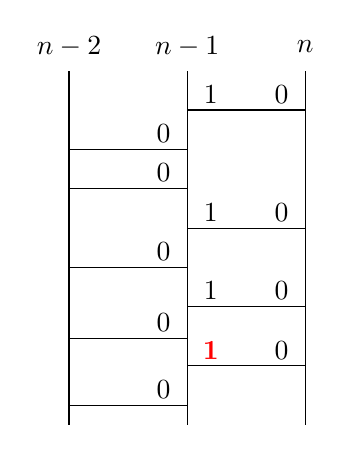
\begin{tikzpicture}
        \draw(0, -0.5) to (0, 4);
            \node at (0, 4.3){$n-2$};
            \draw(0, 3) to (1.5, 3);
                \node at (1.2, 3.2){$0$};
            \draw(0, 2.5) to (1.5, 2.5);
                \node at (1.2, 2.7){$0$};
            \draw(0, 1.5) to (1.5, 1.5);
                \node at (1.2, 1.7){$0$};
            \draw(0, 0.6) to (1.5, 0.6);
                 \node at (1.2, 0.8){$0$};
            \draw(0, -0.25) to (1.5, -0.25);
                \node at (1.2, -0.05){$0$};
        \draw(1.5, -0.5) to (1.5, 4);
            \node at (1.5, 4.3){$n-1$};
            \draw(1.5, 3.5) to (3, 3.5);
                \node at (1.8, 3.7){$1$};
                \node at (2.7, 3.7){$0$};
            \draw(1.5, 2) to (3, 2);
                \node at (1.8, 2.2){$1$};
                \node at (2.7, 2.2){$0$};
            \draw(1.5, 1) to (3, 1);
                \node at (1.8, 1.2){$1$};
                \node at (2.7, 1.2){$0$};
            \draw(1.5, 0.25) to (3, 0.25);
                \node at (1.8, 0.45){$\textcolor{red}{\textbf{1}}$};
                \node at (2.7, 0.45){$0$};

        \draw(3, -0.5) to (3, 4);
            \node at (3, 4.3){$n$};
    \end{tikzpicture}
    \caption{The line coding for $LC_{N-1}$ with imrpovement three is $101110$\underline{$0$}. The red, bold $1$ represents 
    the last left end point in $LC_{N-1}$, therefore the proceeding $0$ must be 
    included in $LC_{N-1}$. For every other $1$ in $LC_{N-1}$, a $0$ is omitted following 
    said $1$.}
    \label{fig:improvement3}
\end{figure}
\paragraph{Combining All Three}
The combination of all three improvements can be done independently. 
Let $IC_{L_{(4,2,3,1)}}$ be the \emph{improved line-based encoding} for $L_{(4,2,3,1)}$ 
by applying improvements 1-3 to $LC_{L_{(4,2,3,1)}}$. Recall that $LC_{L}$ denotes the line-based encoding for some ladder $L$.
$LC_{L_{(4,2,3,1)}}$ for the ladder in Fig. \ref{fig:line-encoding} is $11\underline{0}10101\underline{0}0010101\underline{0}000$.
By applying imrpovement one, we get $11\underline{0}101011\underline{0}0010101\underline{0}$. 
Notice how the last three $0s$ from $LC_{L}$ were removed because they represented $LC_{N}$.
By applying imrpovement two to improvememt one we get $11\underline{0}10011\underline{0}001001\underline{0}$.
Notice how the second, and eigth $1$ were removed because they are implied by 
the successive $0s$. By applying improvement three to the result of improvement 
two we get $11\underline{0}10011\underline{0}00101\underline{0}$. Notice how the last $0$ 
was removed from improvement two. This is because the $0$ is implied in $LC_{N-1}$
due to the configuration between of bars connecting lines $N-1$ and line $N$. The $IC_{L_{(4,2,3,1)}}$ for the ladder in fig. \ref{Fig:allthree} 
is $IC_{L_{(4,2,3,1)}}=11\underline{0}10011\underline{0}00101\underline{0}$.\pagebreak

\begin{figure}[!htp]
     \centering
    \begin{tikzpicture}
         \draw(0, 0) to (0, 4);
             \node at (0, 4.3){$n-3$};
             \draw(0, 3.5) to (1.5, 3.5);
             \draw(0, 2.5) to (1.5, 2.5);
         \draw(1.5, 0) to (1.5, 4);
             \node at (1.5, 4.3){$n-2$};
             \draw(1.5, 3) to (3, 3);
             \draw(1.5, 3.8) to (3, 3.8);
             \draw(1.5, 2) to (3, 2);
             \draw(1.5, 1) to (3, 1);
         \draw(3, 0) to (3, 4);
             \node at(3, 4.3){$n-1$};
             \draw(3, 2.5) to (4.5, 2.5);
             \draw(3, 1.5) to (4.5, 1.5);
             \draw(3, 0.5) to (4.5, 0.5);
         \draw(4.5, 0) to (4.5, 4);
             \node at(4.5, 4.3){$n$};
     \end{tikzpicture}
     \caption{A ladder used to illustrate all three improvements $IC_{L}$. $IC_{L}=11\underline{0}10011\underline{0}00101\underline{0}$}
     \label{Fig:allthree}
\end{figure}
\section{Enumeration, Counting, and Random Generation of \newline Ladder Lotteries}

In the paper, Enumeration, Counting, and Random Generation of Ladder Lotteries~\cite{A6}, written by Nakano and Yamanaka 
the authors consider the problem of enumeration, counting and 
random generation of ladder lotteries with $n$ lines and $b$ bars. 
It is important to note that the authors considered both optimal and 
non-optimal ladders for this paper. Nonetheless, the paper is still fruitful 
for its modelling of the problems and insights into ladder lotteries.
The authors use  the line-based encoding, $LC(l)$ for the representation of ladders 
that was discussed in the review of Coding Ladder Lotteries~\cite{A5}.

%%Section for enumeration
\subsection{Enumeration}
The authors denote a set of ladder lotteries with $n$ lines and 
$b$ bars as $S_{n,b}$. The problem is how to enumerate all the 
ladders in $S_{n,b}$. The authors use a \emph{forest structure}
to model the problem. A \emph{forest structure} is a set of trees 
such that each tree in the forest is disjoint union with every other 
tree in the forest. Consider $S_{n,b}$ to be a tree in a forest.
That is to say, a union disjoint subset of all ladders with $n$
lines and $b$ bars. Then $F_{n,b}$, or the forest of all $S_{n,b}$,
is the union of all disjoint trees of ladders with $n$ lines and $b$ bars. 
%For an example 
% of a forest for $F_{3,2}$ refer to Figure~\ref{fig:forest3,2}.\pagebreak %figure number.
% \begin{figure}[t]
%     \begin{center}
%     \begin{minipage}{.8\textwidth}
%         \begin{tikzpicture}
%             \draw(0, 0) to (0, 2);
%             \draw(0.5, 0) to (0.5, 2);
%                 \node at(0.25, -0.5){00};

%             %%branch
%             \draw[line width=0.5mm] (0.8, 1) to (1.3, 1);

%             \draw(1.5, 0) to (1.5, 2);
%                 \draw(2, 1.5) to (2.25, 1.5);
%             \draw(2, 0) to (2, 2);
%                 \node at (1.75, -0.5){0\underline{1}0};
    
%             %%branch
%             \draw[line width=0.5mm] (2.3, 1) to (2.8, 1);
            
%             \draw(3, 0) to (3, 2);
%             \draw(3.5, 0) to (3.5, 2);
%                  \draw(3.5, 1.5) to (3.75, 1.5);
%                  \draw(3.5, 1) to (3.75, 1);
%                 \node at (3.25, -0.5){01\underline{1}0};
            
%             \draw[line width=0.5mm] (4, 1) to (4.5, 1);

%             \draw(4.6, 0) to (4.6, 2);
%             \draw(5.1, 0) to (5.1, 2);
%             \draw(5.6, 0) to (5.6, 2);
%                  \draw(5.1, 1.5) to (5.35, 1.5);
%                  \draw(5.1, 1) to (5.35, 1);
%                 \node at (5.1, -0.5){011\underline{0}0};


%             \draw[line width=0.5mm](5.8, 1) to (6.3, 1);
%             \draw(6.5, 0) to (6.5, 2);
%             \draw(7, 0) to (7, 2);
%             \draw(7.5, 0) to (7.5, 2);
%                 \draw(7, 1.5) to (7.5, 1.5);
%                 \draw(7, 1) to (7.25, 1);
%                 \node at (7, -0.5){0110\underline{0}0};

%             \draw[line width=0.5mm](7.8, 1) to (8.3, 1);
%             \draw(8.6, 0) to (8.6, 2);
%             \draw(9.1, 0) to (9.1, 2);
%             \draw(9.6, 0) to (9.6, 2);
%                 \draw(9.1, 1.5) to (9.6, 1.5);
%                 \draw(9.1, 1) to (9.6, 1);
%                 \node at (9.1, -0.5){01100\underline{0}0};

%         \end{tikzpicture}
        
%     \end{minipage}
%     \end{center}
    
    
  

%     %%second tree
%     \begin{center}
%           \begin{minipage}{0.8\textwidth}
%             \begin{tikzpicture}
%                 \draw(0, 0) to (0, 2);
%                 \draw(0.5, 0) to (0.5, 2);
%                     \draw(0, 1) to (0.25, 1);
%                     \node at (0.25, -0.5){$100$};
                
%                 %%upper subtree
%                 \draw[line width=0.5mm](0.8, 1.5) to (1.3, 2);
%                     \draw(1.5, 1.5) to (1.5, 3.5);
%                     \draw(2, 1.5) to (2, 3.5);
%                         \draw(1.5, 3) to (2, 3);
%                         \node at (1.75, 1){$10\underline{0}0$};

%                     \draw[line width=0.5mm](2.3, 2.5) to (2.8, 2.5);
%                         \draw(3, 1.5) to (3, 3.5);
%                             \draw(3, 3) to (3.5,3);
%                             \draw(3.5, 2.5) to (3.75, 2.5);
%                         \draw(3.5, 1.5) to (3.5, 3.5);
%                         \node at (3.5, 1){$100\underline{1}0$};

%                     \draw[line width=0.5mm](4, 2.5) to (4.5, 2.5);
%                         \draw(4.7,  1.5) to (4.7, 3.5);
%                             \draw(4.7, 3) to (5.2, 3);
%                             \draw(5.2, 2.5) to (5.45, 2.5);
%                         \draw(5.2, 1.5) to (5.2, 3.5);
%                         \draw(5.7, 1.5) to (5.7, 3.5);
%                         \node at (5.2, 1){$1001\underline{0}0$};

%                     \draw[line width=0.5mm](6, 2.5) to (6.5, 2.5);
%                         \draw(6.8,  1.5) to (6.8, 3.5);
%                             \draw(6.8, 3) to (7.3, 3);
%                             \draw(7.3, 2.5) to (7.8, 2.5);
%                         \draw(7.3, 1.5) to (7.3, 3.5);
%                         \draw(7.8, 1.5) to (7.8, 3.5);
%                         \node at (7.3, 1){$10010\underline{0}0$};



%                 %%lower subtree
%                 \draw[line width = 0.5mm](0.8, 0.5) to (1.3, 0);
%                     \draw (1.5, -0.5) to (1.5, -2.5);
%                         \draw(1.5, -1.5) to (1.75, -1.5);
%                         \draw(2, -1) to (2.25, -1);
%                     \draw(2, -0.5) to (2, -2.5);
%                         \node at (1.5, -2.8){$10\underline{1}0$};
                    
%                     \draw[line width = 0.5mm](2.55, -1.5) to (3.05, -1.5);

%                      \draw (3.3, -0.5) to (3.3, -2.5);
%                         \draw(3.3, -1.5) to (3.8, -1.5);
%                         \draw(3.8, -1) to (4.05, -1);
%                     \draw(3.8, -0.5) to (3.8, -2.5);
%                         \node at (3.6, -2.8){$101\underline{0}0$};

%                      \draw[line width = 0.5mm](4.25, -1.5) to (4.75, -1.5);

%                      \draw (5, -0.5) to (5, -2.5);
%                         \draw(5.5, -1) to (5.75, -1);
%                         \draw(5, -1.5) to (5.5, -1.5);
%                     \draw(5.5, -0.5) to (5.5, -2.5);
%                     \draw(6, -0.5) to (6, -2.5);
%                         \node at (5.5, -2.8){$1010\underline{0}0$};
                    

%                     \draw[line width = 0.5mm](6.3, -1.5) to (6.8, -1.5);
%                     \draw (7.1, -0.5) to (7.1, -2.5);
%                         \draw(7.1, -1.5) to (7.6, -1.5);
%                         \draw(7.6, -1) to (8.1, -1);
%                     \draw(7.6, -0.5) to (7.6, -2.5);
%                     \draw(8.1, -0.5) to (8.1, -2.5);
%                         \node at (7.6, -2.8){$10100\underline{0}0$};
                    

                    
%             \end{tikzpicture}
            
%         \end{minipage}
%     \end{center}


%     \begin{center}
%         \begin{minipage}{0.8\textwidth}
%             \begin{tikzpicture}%% start pocture
            
            
%                 \draw(0, 0) to (0, 2);
%                     \draw(0, 1.5) to (0.25, 1.5);
%                     \draw(0, 1) to (0.25, 1);
%                 \draw(0.5, 0) to (0.5, 2);
%                 \node at (0.25, -0.5){$1100$};
            
            
%                 \draw[line width=0.5mm] (0.8, 1) to (1.3, 1);
%                     \draw(1.5, 0) to (1.5, 2);
%                         \draw(1.5, 1.5) to (2, 1.5);
%                         \draw(1.5, 1) to (1.75, 1);
%                     \draw(2, 0) to (2, 2);
%                     \node at (1.75, -0.5){$110\underline{0}0$};
            
        
%                 \draw[line width=0.5mm] (2.3, 1) to (2.8, 1);
%                     \draw(3, 0) to (3, 2);
%                        \draw(3, 1.5) to (3.5, 1.5);
%                        \draw(3, 1) to (3.5, 1);
%                    \draw(3.5, 0) to (3.5, 2);
%                     \node at (3.25, -0.5){$1100\underline{0}0$};
            
            
%                 \draw[line width=0.5mm] (3.8, 1) to (4.3, 1);
%                     \draw(4.5, 0) to (4.5, 2);
%                           \draw(4.5, 1.5) to (5, 1.5);
%                           \draw(4.5, 1) to (5, 1);
%                       \draw(5, 0) to (5, 2);
%                       \draw(5.5, 0) to (5.5, 2);
%                           \node at (5, -0.5){$11000\underline{0}0$};
               
%             \end{tikzpicture}%%end picture
%         \end{minipage}
%     \end{center}
%     \caption{The forest, $F_{3,2}$ where $3$ is the number of lines and $2$ is the number of bars. All ladders with $3$ lines and $2$ bars are leaf nodes of one of three trees $S_{3,2}$.
%     The underlined bits are the inserted second last bit from the parent's line-encoding resulting in the child's line encoding}
%     \label{fig:forest3,2}
% \end{figure}

%%end enumeratiom section

%%section for counting
\subsection{Counting}
The authors provide a method and algorithm to count all ladders 
with $n$ lines and $b$ bars. The counting algorithm 
works by dividing ladders into four types of sub-ladders.
For sub-ladder, $r$, its type is a tuple $t(n,h,p,q)$ where 
$n$ is the number of lines, $h$ is the number of half bars, 
$p$ is the number of unmatched end-points on line $n-1$ and 
$q$ is the number of unmatched end-points on line $n$. From this 
type, the authors are able to count all ladders with $n$ lines and $b$ bars. 
% \subsubsection{ $h < p+q$ or $n<2$}
% There are zero ladders because it is impossible for the 
% root sub-ladder to have less than two lines. It is also 
% impossible for the number of half bars, $h$, to 
% be less than the number of detached left end points 
% on line $n-1$ plus the number of detached end points on 
% line $n$.

% %%\subsubsubsection{Case 2: $n=2$ and $h=p$ and $q=0$}
% \subsubsection{$n=2$ and $h=p$ and $q=0$}
% There is only one ladder because the number of half bars 
% on the last line is 0 since $q=0$. Therefore all half bars are on the 
% $n-1th$ line of the sub-ladder. This is known because 
% $h=p$ which means the number of half bars is the same as 
% the number of unmatched bars on line $n-1$. Hence, the unmatched 
% half bars on the $n-1th$ line must be connected to the $n$ 
% line. Once these are all matched the ladder will be complete. 
% Thus, there is only one ladder for this case.

% %%\subsubsubsection{Case 3: $(n \geq 3$ or $h>p)$ and $q=0$}
% \subsubsection{$(n \geq 3$ or $h>p)$ and $q=0$}
% If this is the case, then there are no endpoints attached to 
% line $n$, but the number of half bars is greater than the 
% number of endpoints attached to line $n-1$, which means there is 
% some line(s) $n-t$, $t>2$ that have end points attached to them.
% Let $r$ be a sub-ladder of type $r=t(n,h,p,q)$
% with the the above values for $n,h,p,q$. In order to count the number of ladders of type 
% $t(n\geq3, h>p, q=0)$ the authors demonstrate an injection $|t(n\geq3, h>p, q=0)|=|t(n-1,h,0,p)| + |t(n,h-1,p+1,q)|$.\cite{A6}
% Let $P(r)$ be $r$ with the removal of $r's$ second last bit in $LC(r)$; i.e. the parent of 
% $r$.  The $LC(r)$ must have a $0$ for the second last bit. This $0$ designates either the 
% end of line $n-1$ or a right endpoint of a bar attached to line $n-1$. 
% If the second last bit in $LC(r)$ is the right end point of some 
% bar, then $P(r)=t(n,h-1,p+1,q)$. This is because the $n-1th$ bar 
% has a right end point that must be connected to some left  
% endpoint at line $n-2$. Since the removal sequence of the second 
% last bit ensures that there cannot be a right end-point detached 
% from a left end-point. Only left end-points can be detached 
% from right end-points~\cite{A6}. However, if the second last bit 
% of $LC(r)$ designates the end of line $n-1$, then $P(r)=t(n-1,h,0,p)$. 
% This is because the removal of the second last bit 
% is the removal of the end of line $n-1$ in $r$. Thus, 
% line $n$ must be empty in $r$ since the last bit in $LC(r)$
% designated the end of line $n$. Thus, if line $n$ is empty 
% and the end point of line $n-1$ has been removed from $LC(r)$, 
% resulting in $P(LC(r))$, the last bit in $P(LC(r))$ must be 
% the end of line $n-1$ in $r$ resulting in a pre-ladder with one 
% less line than $r$.\par  

% \subsubsection{ $h\geq p+q$ and $q>0$}
% %%\subsubsubsection{Case 4: $h\geq p+q$ and $q>0$}
% Let $r$ be a pre-ladder of type $t(n,h,p,q)$. The authors 
% demonstrate $|t(n,h\geq p+q,q>0)|=|t(n,h-1,p+1,q)|+|t(n,h-1,p,q-1)|$.\cite{A6} 
% The second last bit of $LC(r)$ is either a $0$ 
% or a $1$. If it is a $0$ then it represents a 
% right end point attached to line $n$. Thus, 
% removing it to get $P(LC(r))$ is in effect 
% detaching a right end point from some left end point 
% on line $n-1$. Therefore, the parent, $P(R)$ is 
% of type $t(n,h-1,p+1,q)$. Seeing as in the parent, 
% there is now a left end point detached from its right 
% end point in $r$. However, if the second last bit 
% of $LC(r)$ is a $1$, then this indicates the left 
% half of a bar on line $n$. But since there is no 
% bar $n+1$, this left end point must be detached. 
% Therefore, by removing this $1$ in $LC(r)$ results 
% in a parent with one less detached end point on line $n$.
% Thus $P(R)$ is of type $t(n,h-1,p,q-1)$.
% \subsection{Random Generation}
% The random generation of ladder lotteries with $n$ lines and
% $b$ bars is done by the recurrence relations in the counting 
% and enumerating sections. The goal is to produce 
% some $L$ of type $t(n,2b,0,0)$ where the number of half 
% bars equals the total $2(b)$ and there are no detached 
% end points on lines $n-1$ and $n$. This implies that there 
% are no detached endpoints on any line $n-t$ where $t\geq2$
% because the removal sequence from the $LC(pre-ladder)$
% ensures that any line before $n-1$ has no detached endpoints. Thus, 
% if $L$ is of type $t(n,2b,0,0)$ it is no longer a pre-ladder 
% but a complete ladder with $n$ lines and $b$ bars~\cite{A6}.\par 
% The authors use an algorithm to generate a random integer, $x$,
% in the range of $[1 \dots |t(n,h,p,q)|]$. where $t(n,h,p,q)$ corresponds to some 
% parent type of ladder. $t(n1,h1,p1,q1)$ corresponds to one 
% child type of $t(n,h,p,q)$ and $t(n2,h2,p2,q2)$ corresponds 
% to the other child type. If $x\leq|t(n1,h1,p1,q1)|$ then generate 
% a pre-ladder of type $t(n1,h1,p1,q1)$ else generate a pre-ladder 
% of type $t(n2,h2,p2,q2)$~\cite{A6}. Continue until there is type $t(n,2b,0,0)$
% which corresponds to a complete ladder lottery with $n$ lines and $b$ bars.
\section{Permutations}
Ladder lotteries and permutations are intricately related to each other. Each $\pi$ has an $OptL\{\pi\}$ such that 
each ladder form $OptL\{\pi\}$ sorts $\pi$. The so called Listing Problem is one of the problems addressed in this thesis.
In brief, this problem is about how to list all $n!$ ladders efficiently. The research for this problem is highly influenced 
by permutation enumeration research. Knuth describes a number of 
permutation enumeration algorithms in The Art of Computer Programming~\cite{A18}. Since this book, many algorithms for 
enumerating $n!$ permutations have been created. During my research for the Listing Problem, I investigated nine of these 
enumeration algorithms\cite{A18}\cite{A19}\cite{A21}\cite{A24}\cite{A25}\cite{A26}\cite{A31}\cite{A34}\cite{A35}. 
The first is the lexicographic algorithm which orders all $n!$ permutations from smallest to largest. The lexicographic 
algorithm generates each permutation with an amortized time of $O(n^{2}log(n))$~\cite{A21}. The second of which is the 
colexicographic algorithm which orders all $n!$ permutations from largest to smallest. The colexicographic 
algorithm generates each permutation with an amortized time of $O(n^{2}log(n))$~\cite{A19}. The third of which is Zak's 
algorithm which generates all $n!$ permutations by reversing a suffix in one permutation to get to the next 
permutation. The time complexity of Zak's algorithm is amortized time of $O(n^{2})$~\cite{A31}.
The fourth of which is Heap's algorithm which is a decrease and conquer algorithm.  
The algorithm is based on rotating elements in an array such that the $nth$ position 
is occupied by the $nth$ element for all permutations of the $(n-1)$ objects. 
Then the $nth$ element is swapped with one of the elements of in the first $(n-1)$ positions.
The process repeats itself until all of the $n$ elements have occupied the $nth$ position exactly once. 
The time complexity of Heap's algorithm is {\sc CAT}, constant amortized time of $O(1)$ per permutation~\cite{A24}.
The fifth algorithm is Corbett's algorithm which rotates a prefix of the first possible length in 
$n$,$2$,$n-1$,$3$,$n-2$,$4$, etc.~\cite{A34}. The sixth algorithm is 
the algorithm using star transpositions that always swaps the first element of the permutation with some other element. 
It was discovered by Gideon Ehrlich and is described as Algorithm E in Knuth's book~\cite{A18}.
The seventh algorithm is the derangement ordering in which no two consecutive permutations have any elements 
in the same position~\cite{A35}. The Steinhaus-Johnson-Trotter algorithm generates $S_{n}$ by performing adjacent swap operations 
on the permutation resulting in the next permutation. Thus, each permutation in $S_{n}$ differs 
from it predecessor by a single swap operation~\cite{A25}.
Effler and Ruskey's algorithm lists permutations by groups of $k$ inversions. Their algorithm has 
constant amortized time algorithm for generating permutations of order $n$ with $k$ inversions~\cite{A26} meaning 
the time it takes to generate each permutation is bounded by a constant.
The algorithm is also a \emph{BEST} algorithm (backtracking ensures success at terminals), meaning that when the algorithm backtracks, 
the back-tracking leads to a successful result~\cite{A26}.\par 
In Chapter 1, it was already stated that Algorithms~\cite{A25}\cite{A26} were the most conducive for The Listing Problem. 
These are the Steinhaus-Johnson-Trotter and Effler-Ruskey algorithms respectively. Each of these two algorithms are 
advantageous for differing reasosns. The reason that the SJT algorithm is beneficial is because it generates each 
permutation in $O(1)$ per ladder; thus making it extremely efficient. In Chapter 3, the SJT 
algorithm is modified to create ladders instead of permutations while still maintaining the same efficiency.
The reason that the Effler-Ruskey algorithm 
is beneficial is because it has a nice ordering property in which the permutations are listed by the number of inversions.
The algorithm is still fairly efficient due to it being BEST and CAT. In Chapter 3, the Effler-Ruskey algorithm 
is modified to create ladders by $k$ bars, though in doing so it loses some of the efficiency of permutation listing algorithm.
Below, the details of the SJT and Effler-Ruskey algorithms for permutations will be analyzed in detail.

\subsection{Lexicographic Algorithms}

%%
\subsubsection{Basic Lexicographic Algorithm}
The lexicographic algorithm enumerates permutations from smallest to largest. The lexicographic order for $S_{3}$ is $(1,2,3),(1,3,2),(2,1,3),(2,3,1),(3,1,2),(3,2,1)$.
This is the same way the words in a dictionary are ordered in the sense that $a < b < c \dots y < z$.
There are many algorithms for enumerating permutations lexicographically~\cite{A19, A20, A21, A22, A23}. 
Several will be discussed in this thesis. The first of which is the basic lexicographic ordering algorithm.
Please refer to Algorithm~\ref{Alg:BasicLex} to see the basic lexicographic listing algorithm.\pagebreak
\begin{algorithm}
    \begin{algorithmic}[1]
        \Function{Basic Lex}{$\pi$, $n$}
            \For{$i$ \textbf{from} $n$ \textbf{to} $1$}
                \If{$p_{i} > p_{i-1}$}
                    \State \small{$v \gets$ the index of the minum value greater than $p_{i-1}$ and
                    to the right of $p_{i-1}$}
                    \State {\sc Swap}$(p_{i-1}, p_{v})$
                    \State {\sc Sort}$(p_{i},p_{i+1} \dots p_{n})$
                    \State {\sc BaiscLex($\pi$, $n$)}
                   
                \EndIf
            \EndFor
          

        \EndFunction
        
    \end{algorithmic}
    \caption{The Basic Lexicographic Algorithm}
    \label{Alg:BasicLex}
\end{algorithm}
This algorithm works by beginning with the identity permutation of order $n$. Then going right to left, 
it finds an increasing substring of size two. Once found, the algorithm finds the index of the smallest value greater than the 
value at index $i-1$ in $\pi$ to the right of index $i-1$; let this index be known as $v$. 
Then the algorithm swaps $v$ and $p_{i-1}$ in $\pi$. The algorithm sorts $\pi$ from index $i$ to index $n$ and a recursive call is made.
The algorithm terminates when $\pi$ is in descending order. The 
algorithm generates each permutation with an amortized time of 
$O(n^{2}log(n))$. The for loop runs between $0$ to $n$ times per function call which accounts for the $n$ factor. 
The right portion of the permutation needs to be sorted on every function call. Sorting is done in $nlog_{n}$ time. 
$n*nlog_{n}$ is simplified to $n^{2}log_{n}$.




%%p2
\subsubsection{Alternating Lexicographic Algorithm}
In the paper Generating Alternating Permutations Lexicographically, written by Bauslaugh and Ruskey, the authors provide an algorithm 
for generating permutations in lexicographic ordering such that the permutations form a zig-zag pattern. 
The zig-zag pattern is formally defined as follows, given $\pi$ of order $n$:  If $n = 2K$ then 
zig-zag = $p_{1} < p_{2} > p_{3} < p_{4} \dots p_{n-1} < p_{n}$. 
If $n= 2K+1$ then zig-zag = $p_{1} < p_{2} > p_{3} < p_{4} \dots p_{n-1} > p_{n}$~\cite{A19}.
Please refer to Algorithm~\ref{Alg:AltLex} to see the Alternating Lexicographic Algorithm.
The initial values for the function are $m=n$, $val=1$, $level=0$ and $S = \{1 \dots n\}$ and $\pi=()$.


\begin{algorithm}
    \begin{algorithmic}[1]
        \Function{AlternatingLex}{$m$,$val$,$level$, $S=\{1 \dots n\}$, $\pi$}
            \State $p_{level} \gets val$
            \State $S \gets S-\{val\}$
            \If{$m = 1$}
                \State {\sc print($\pi$)}
                \State \textbf{return}
            \EndIf
            \State $T \gets \{\}$
            \If{$level=2k+1$}
                \State $T \gets \{x \in S | x < S_{max}$ \textbf{and} $x < val\}$
            \Else 
                \State $T \gets \{x \in S | x > S_{min}$ \textbf{and} $x > val\}$
            \EndIf
            \For{$x \in T$}
                \State {\sc AlternatingLex($m-1$, $x$, $level+1$, $S - \{x\}$, $\pi$)}
            \EndFor
        \EndFunction
        
    \end{algorithmic}
    \caption{Alternating Lexicographic Enumeration Algorithm}
    \label{Alg:AltLex}
\end{algorithm}


On each function call $val$ is inserted into $\pi$ at $level$. Then $val$ is removed from $S$.
If $level$ is odd then the set $T$ gets every value from $S$ less than the max value in $S$ and 
less than $val$. If  $level$ is even then $T$ gets every value from $S$ greater than  the min value 
in $S$ and greater than $val$. Then, for each $x$ in $T$, the function makes a recursive call 
with $m$ equal to $m-1$, $k$ equal to $x$, $level$ equal to $level+1$ and $S$ equal to $S$ without 
element $x$. To see the permutations of order $5$ generated by the alternating lexicographic algorithm, 
please refer to Table~\ref{Table:AltPerms}.

\begin{center}
\begin{table}
\begin{tabular}{ |p{3cm}||p{3cm}|p{3cm}|p{3cm}|  }
 \hline
 \multicolumn{4}{|c|}{Alternating Permutations of order $5$} \\
 \hline
 \hline
 13254   & 14253    &14352&  15243\\\hline
 15342&  23154  & 24153   &24351\\\hline
 25143 &25341 & 34152&  34251\\\hline
 35142    &35241 & 45132&  45231\\
 \hline
\end{tabular}
\label{Table:AltPerms}
\end{table}
\end{center}

The authors state that the algorithm is constant amortized time which means the total amount of
computation done in generating all the objects, divided by the number of objects, is
bounded by a constant. On the average and up to a constant factor no algorithm can
run faster~\cite{A19}. The constant refers to the number of function calls before the algorithm terminates. It is defined as follows. 
Let $AL$ denote the recurrence relation for the Alternating Lexicographic algorithm, let $k$ denote the 
first element in $\pi$ and let $n$ denote the number of elements in the set. 
If $n=1$ and $K=1$ then $AL(n, K)=0$. If $n=n$ and $K=n-1$ then $AL(n,K)= 1 + AL(n-1,1)$ For all other cases, 
then $AL(n, K) = AL(n, K+1) + A(n-1, n-K)$~\cite{A19}.

% \subsubsection{Parallelized Lexicographic Algorithms}
% The lexicographic listing algorithm can be improved by parallelizing the process. There are a number of algorithms for 
% parallelizing the lexicographic listing problem. These algorithms are found in the following papers~\cite{A21, A22, A23, A24}.
% Rather than go through these papers one by one, a more general approach to parallelized solutions of the 
% lexicographic listing problem will be provided.\par 
% The general solution to the problem is to partition the $n$ elements into $M$ procecssors, then have each processor 
% list $(n/M)!$ subsets of elements. Though these algorithms are interesting, the analysis of these algorithms was not 
% pertinent to the research in this thesis, seeing as the Listing Problem runs on a single processor.

\subsection{Heap's Algorithm}
Heap's algorithm was developed by B.R. Heap in 1963~\cite{A24}. 
The algorithm is based on rotating elements in an array such that the $nth$ position 
is occupied by the $nth$ element for all permutations of the $(n-1)$ objects. 
Then the $nth$ element is swapped with one of the elements of in the first $(n-1)$ positions.
The process repeats itself until all of the $n$ elements have occupied the $nth$ position exactly once. 
The element occupying the $nth$ position is swapped with the element in the first position if $n$ 
is even. The element occupying the $nth$ position is swapped with $p_{i}$ if $n$ is odd.
To see Heap's algorithm please refer to Algorithm~\ref{Alg:Heaps}. The initial conditions 
for {\sc Heaps} are the following. Let $\pi$ be initialized to the identity permutation 
of order $n$. Let $n$ be the number of elements in $\pi$ from $[1 \dots n]$. $n$ is 
reduced by $1$ on each recursive call until $n=1$. On each function call the length of 
$\pi$ is reduced by one such that the first $n-1$ elements of $\pi$ are considered and the 
$nth$ element of $\pi$ is ignored.

\begin{algorithm}
    \begin{algorithmic}[1]
        \Function{Heaps}{$\pi$, $n$}
            \If{$n=1$}
                \State \textbf{return}
            \Else 
                \For{$i$ \textbf{from} $1$ \textbf{to} $n$}
                    \State {\sc Heaps($\pi$, $n-1$)}
                    \State {\sc Print($\pi$)}
                    \If{$n = 2k+1$}
                        \State {\sc Swap($p_{1}$, $p_{n}$)}
                    \Else 
                        \State {\sc Swap($p_{i}$, $p_{n}$)}
                    \EndIf
                \EndFor
            \EndIf
        \EndFunction
        
    \end{algorithmic}
    \caption{Heaps Algorithm for Generating all $n!$ Permutations}
    \label{Alg:Heaps}
\end{algorithm}

The time complexity for {\sc Heaps} algorithm is $O(1)$ constant amortized time per permutation. For each value of $n=[1 \dots n]$, 
the algorithm makes $n$ recursive calls, each of which produces all $(n-1)!$ permutations of 
order $(n-1)$ in $O(1)$ time per permutation. The exception is prior to outputting the first permutation, in which 
the function produces $n=${\sc Max($\pi$)} recursive calls before the first permutation is output.


\subsection{Zak's Algorithm}
Zak's Algorithm was first written about by Shmuel Zak's in the paper A new Algorithm For
Generation Of Permutations~\cite{A31}.The algorithm is based on reversing suffixes in a permutation 
of different sizes until all $n!$ permutations have been listed. The algorithm makes 
use of a \emph{suffix vector} which is a vector for holding all the suffix sizes to be reversed. 
Since there are $n!$ permutations, there are $n!$ non-unique suffix sizes held in the suffix vector.
The recurrence relation for the suffix sizes is as follows. Let $S(n)$ denote the suffix of size $n$. 
Then we get the following recurrence relation for $S(n)$. If $n=2$ then $S(n)=2$, else 
$S(n)=(S(n-1)n)^{n-1}S(n-1)$. Let \emph{suffixVector} be initialized to an empty vector holding integers. If $n$ equals 
two, append $2$ to \emph{suffixVector}, else append \emph{suffixVector[n-1]} to 
\emph{suffixVector}, followed by appending $n$ to \emph{suffixVector}, $n-1$ times. 
Lastly, append \emph{suffixVector} at $n-1$ to \emph{suffixVector}~\cite{A31}
 Once the \emph{suffixVector} has been created, for each integer in the \emph{suffixVector}, reverse 
the suffix of that size in $\pi$. To see Zak's Algorithm for creating the suffix vector please refer to 
Algorithm~\ref{Alg:Zaks}\pagebreak
\begin{algorithm}[t]
    
    \begin{algorithmic}[1]
        \Function{SuffixVector}{\textit{suffixVector}, $n$}
        \If{$n=2$}
           \State append $2$ to \textit{suffixVector}
        
        \Else 
            \For{$i$ \textbf{from} $1$ \textbf{to} $n$}
                \State append {\sc SuffixVector(\textit{suffixVector}, $n-1$)} to \textit{suffixVector}
                \State append $n$ to \textit{suffixVector}
            \EndFor
            \State append {\sc SuffixVector(\textit{suffixVector}, $n-1$)} to \textit{suffixVector}
        \EndIf
        \EndFunction
    \end{algorithmic}
    \begin{algorithmic}[1]
        \Function{Zaks}{\textit{suffixVector}, $\pi$}
            \For{\textbf{each} $x$ $\in$ \textit{suffixVector}}
                \State {\sc Print($\pi$)}
                \State reverse suffix of size$=x$ in $\pi$
            \EndFor
            \State {\sc Print($\pi$)}
        \EndFunction
    \end{algorithmic}
    \caption{Zaks algorithm for creating all $n!$ permutations.}
    \label{Alg:Zaks}
\end{algorithm}




%Paragraph SJT
\subsection{Steinhaus-Johnson-Trotter Algorithm}
The Steinhaus-Johnson-Trotter algorithm generates $S_{n}$ by performing adjacent swap operations 
on the permutation resulting in the next permutation. Thus, each permutation in $S_{n}$ differs 
from it predecessor by a single swap operation~\cite{A25}. This makes the SJT algorithm a very efficient 
algorithm for listing $S_{n}$. Let an \emph{even permutation} be defined as a permutation 
with an even number of inversion. Let an \emph{odd permutation} be defined as a 
permutation with an odd number of inversions. The $nth$ element is inserted into all 
positions of $\pi$ of order $n-1$ in descending order if $\pi$ of order $n-1$ is an even permutation.
The $nth$ element is inserted into all positions of $\pi$ of order $n-1$ in ascending order if 
$\pi$ of order $n-1$ is an odd permutation~\cite{A25}. For $\pi$ of order $1$ we have $\pi=(1)$. Since 
there are no inversions in $\pi=(1)$ it is even. Now insert $2$ in all positions in $\pi=(1)$
in descending order. Thus we get $(1,2)$ followed by $(2,1)$. Since $(1,2)$ is 
an even permutation, insert $3$ into all positions in descending order resulting in $(1,2,3)$,
$(1,3,2)$ and $(3,1,2)$. Since $(2,1)$ is an odd permutation, insert $3$ 
into all permutations in ascending order resulting in $(3,2,1)$, $(2,3,1)$ and $(2,1,3)$.
Initialize $\pi$ to the identity permutation, initialize $currentElement$ to $2$, initialize 
$n$ to $p_{max}$. Let $direction$ be a Boolean array of size $n$ initialized to $true/right$ for indices. 
If $currentElement$ is greater than $n$, print $\pi$ 
and return. Otherwise, begin a for loop that runs $i=[1 \dots n-1]$ times. 
In the for loop, first make a recursive call with $currentElement$ increasing by one. 
If $direction[currentElement]$ is $right$, then swap $currentElement$ in $\pi$ with its left neighbor. Else 
if $direction[currentElement]$ is $left$ then swap the $currentElement$ in $\pi$ with its right neighbor.
Once the for loop has exited, make one more recursive call with $currentElement+1$ outside the for loop; 
this avoids an extra swap operation from occurring while still maintaining the correct number of recursive 
calls. Lastly, negate $direction[currentElement]$, which effectively changes the direction of the $currentElement$ 
in $direction$ for the next time $currentElement$ is to be swapped. 
To see the Steinhaus-Johnson-Trotter algorithm please refer to Algorithm~\ref{Alg:SJT}.

\begin{algorithm}
    \begin{algorithmic}[1]
        \Function{SJT}{$\pi$, $currentElement$, $n$, $direction$}
            \If{$currentElement > n$}
                \State {\sc Print$(\pi)$}
                \State \textbf{return}
            \EndIf
            \For{$i$ \textbf{from} $1$ \textbf{to} $currentElement-1$}
                \State {\sc SJT($\pi$, $currentElement+1$, $n$)}
                \State $index \gets $ index of $currentElement$ in $\pi$
                \If{$direction[currentElement]=right$}
                    \State $Swap(p_{index}, p_{index-1})$
                \Else 
                    \State $Swap(p_{index}, p_{index+1})$
                \EndIf
            \EndFor
            \State {\sc SJT}($\pi$, $currentElement+1$, $n$, $direction$)
            \If{$direction[currentElement]=right$}
                \State $direction[currentElement] \gets left$
            \Else 
                \State $direction[currentElement] \gets right$
            \EndIf
        \EndFunction
        
    \end{algorithmic}
    \caption{SJT Algorithm for listing $S_{n}$}
    \label{Alg:SJT}
\end{algorithm}

The Steinhaus-Johnson-Trotter algorithm is a Gray Code, meaning that in order to transition 
between any two subsequent permutations in $S_{n}$, there is a minimal amount of constant 
change required. The algorithm simply swaps two elements in order to transition between 
permutations. Each recursive call creates a new permutation with the exception of the 
initial call to the function in which $n$ recursive calls need to be made before the 
first permutation is printed. The amortized time to transition between permutations is $O(1)$.




%%Paragraph 
\subsection{Effler-Ruskey Algorithm}
%%%%%%%%%%FIX ME %%%%%%%%%%%%%%%%
In the paper A CAT Algorithm for Generating Permutations with a Fixed Number of Inversions, written by Effler and Ruskey, the authors provide a 
constant amortized time algorithm for generating all permutations of order $n$ with $k$ inversions~\cite{A26} meaning 
the time it takes to generate each permutation is bounded by a constant.
The algorithm is also a \emph{BEST} algorithm (backtracking ensures success at terminals), meaning that when the algorithm backtracks, 
the back-tracking leads to a successful result~\cite{A26}. 
Let the initial conditions of the algorithm be the following. Let $\pi$ be the empty permutation of order $n$. Let $n$
be initialized as the elements $[1 \dots n]$. Let $k$ be initialized to an integer between $[0 \dots {n \choose 2}]$. 
Let $list$ be initialized to the list of $n$ elements in strictly descending order. 
Let $i$ be the index of element $x$ in $list$. $n-i$ 
indicates the number of inversions formed with $x$ when inserting $x$ into position $n$ in $\pi$.
The algorithm works as follows.
Going right to left in the $list$, each element, $x$, in $list$ is inserted into $p_{n}$
only if inserting $x$ into position $n$ in $\pi$ does not exceed the current number of inversions, $k$. I.E. only 
if $k- (n-i) \geq 0$.
If $x$ is inserted into $\pi$ at position $n$ then $x$ is removed from $list$, a recursive call is made such that $n$ is reduced by 
$1$ and $k$ is reduced by $(n-i)$. When the function returns from its recursive call, element $x$ is placed back into the list 
at its original position. To see the algorithm please refer to Algorithm~\ref{Alg:KInv}.\pagebreak
\begin{algorithm}[t]
    \begin{algorithmic}[1]
        \Function{KInversions}{$\pi$, $n$, $k$, $list$}
            \If{$n = 0$ and $k = 0$}
                \State {\sc Print}($\pi$)
            \Else
                \For{$i$ \textbf{from} length \textbf{of} $list$ \textbf{to} $1$}
                    \State $x \gets list_{i}$
                    \If{$n-i \leq k \leq {n-1\choose k} + (n-i)$}
                        \State $p_{n} \gets x$
                        \State remove $x$ from $list$ 
                        \State $k \gets k - (n-i)$
                        \State {\sc KInversions}$(\pi, n-1, k, list)$
                        \State insert $x$ in $list$ at correct position.
                    \EndIf
                \EndFor
            \EndIf
        \EndFunction
        
    \end{algorithmic}
    \caption{Generate all permutations with $k$ inversions}
    \label{Alg:KInv}
\end{algorithm} 

Below is an example of how the algorithm creates one permutation of order $4$ with $2$ inversions.
\begin{enumerate}
    \item Initial Call: {\sc KInversions}($\pi$=(\underline{ },\underline{ },\underline{ },\underline{ }),$n=4$,$k=2$,$list=[1,2,3,4]$):\newline 
    given $\pi$=(\underline{ },\underline{ },\underline{ },\underline{ }), $n=4$, $k=2$, $list=[1,2,3,4]$, $i=2$ and $x=3$ 
    then inserting $x$ into position $n=4$ would form $4-3=1$ 
    inversion(s). Specifically, the inversion $(4,3)$. Thus, $k$ would be reduced by $1$ in the recursive call 
    and $n$ would be reduced by $1$ in the recursive call. 

    \item First recursive call: {\sc KInversions}($\pi$=(\underline{ },\underline{ },\underline{ },\underline{3}),$n=3$,$k=1$,$list=[1,2,4]$):\newline 
    given $\pi$=(\underline{ },\underline{ },\underline{ },\underline{3}),$n=3$,$k=1$,$list=[1,2,4]$,$i=3$ and $x=4$
    then inserting $x$ into position $3$ would form $3-3=0$ inversions. Thus, $k$ would be reduced by $0$ in the 
    recursive call and $n$ would be reduced by $1$ in the recursive call.

    \item Second recursive call: {\sc KInversions}($\pi$=(\underline{ },\underline{ },\underline{4},\underline{3}),$n=2$,$k=1$,$list=[1,2]$):\newline 
    given $\pi$=(\underline{ },\underline{ },\underline{4},\underline{3}),$n=2$,$k=1$,$list=[1,2]$,$i=1$ and $x=1$
    then inserting $x$ into position $1$ would form $2-1=1$ inversion. Thus, $k$ would be reduced by $1$ to $0$ in the 
    recursive call and $n$ would be reduced by $1$ in the recursive call.

    \item Third recursive call: {\sc KInversions}($\pi$=(\underline{ },\underline{1},\underline{4},\underline{3}),$n=1$,$k=0$,$list=[2]$):
    \newline given $\pi$=(\underline{ },\underline{1},\underline{4},\underline{3}), $n=1$, $k=0$, $list=[2]$ $i=1$ and $x=2$
    then inserting $x$ into position $1$ would form $1-1=0$ inversions. Thus, $k$ would be reduced by $0$
    and $n$ would be reduced by $1$.

    \item Fourth recursive call: {\sc KInversions}($\pi$=(\underline{2},\underline{1},\underline{4},\underline{3}),$n=0$,$k=0$,$list=[]$):\newline 
    Given $n=0$ and $k=0$ the algorithm {\sc Prints}($\pi$) and returns.
\end{enumerate}










%%Sorting Networks File. 

%Intro subsection
\section{Sorting Networks}
Let a \emph{wire} be a horizontal line. Let a \emph{comparator} be a vertical line connecting two wires. A 
\emph{sorting network} is a device consisting of $[1 \dots n]$ wires and $[0 \dots m]$  
comparators such that the sorting network sorts a permutation of $n$ elements into ascending order. The 
$n$ elements are first listed to the left of each wire in the network. The elements travel across their respective wires 
at the same time. When a pair of elements, traveling through a pair of wires, 
encounter a comparator, the comparator swaps the elements if and only if the top wire's element 
is greater than the bottom wire's element. A sorting network with $n$ wires and $m$ 
comparators that can sort any permutation of order $n$ is a \emph{complete sorting network}. 
To see a complete sorting network for $n=4$ please refer to Figure~\ref{Fig:SortNetwork}.\par 

\begin{figure}[h]
   ~\centering
    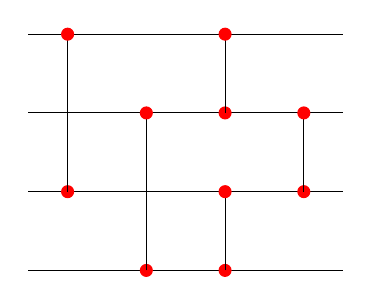
\begin{tikzpicture}
        \draw(0, 0) to (4, 0);
           
        \draw(0, 1) to (4, 1);
        \draw(0, 2) to (4, 2);
           
        \draw(0, 3) to (4, 3);

        %%connector 1
        \draw[red, fill=red](.5,1) circle (.5ex);
            \draw(.5, 1) to (.5, 3);
        \draw[red, fill=red](.5,3) circle (.5ex);


        %%connector 2 
        \draw[red, fill=red](1.5,0) circle (.5ex);
            \draw(1.5, 0) to (1.5, 2);
        \draw[red, fill=red](1.5,2) circle (.5ex);

        %%connector 3
        \draw[red, fill=red](2.5,2) circle (.5ex);
            \draw(2.5, 2) to (2.5, 3);
        \draw[red, fill=red](2.5,3) circle (.5ex);

        \draw[red, fill=red](2.5,0) circle (.5ex);
            \draw(2.5, 0) to (2.5, 1);
        \draw[red, fill=red](2.5,1) circle (.5ex);
        
        %%connector 4
        \draw[red, fill=red](3.5,1) circle (.5ex);
            \draw(3.5, 1) to (3.5, 2);
        \draw[red, fill=red](3.5,2) circle (.5ex);


    \end{tikzpicture}
    \caption{Complete Sorting Network for $n=4$.}
    \label{Fig:SortNetwork}
\end{figure}

Sorting networks were first studied in 1954 by Armstrong, Nelson and O'Connor~\cite{A18}. 
Donald Knuth describes how the comparators for binary integers can be implemented as simple, 
three-state electronic devices~\cite{A18}. Batcher, in 1968, 
suggested using them to construct switching networks for computer hardware, replacing 
both buses and the faster, but more expensive, crossbar switches~\cite{A27}. Currently, sorting networks 
are implemented in graphical processing units, GPUs, for faster sorting methods than traditional CPU sorting methods~\cite{A28}.\par  
Let a \emph{minimum sorting network} be defined 
as a sorting network such that for any arbitrary comparator, $c$, on wire $i$, $c$ connects to line $i+1$ or $i-1$. Furthermore, 
the number of comparators in a minimum sorting network is equal to the number of inversions in $\pi$. Clearly, there is a 
bijection from comparators in a minimum sorting network to the bars in an optimal ladder lottery, and there 
is a bijection from the wires in a minimum sorting network and the lines in a ladder lottery. 


 
\subsection{The Integer Sequence Relating to the Reverse Permutation}
Let $\pi=(n,n-1, \dots 2,1)$ refer to the reverse permutation order $n$. 
There is an integer sequence that counts the number of minimum sorting networks 
for $\pi$. This integer sequence also counts $OptL\{(n,n-1, \dots 2,1)\}$. This sequence grows very quickly, therefore $n=15$ 
is  the largest value this integer sequence has been calculated for. To refer to the table for this sequence 
please refer to Table~\ref{Tab:IntSeq1}~\cite{A30}.
\begin{table}[t]
    \begin{center}

    \begin{tabular}{|p{2cm}||p{8cm}|}
        \hline
        \multicolumn{2}{|c|}{Number of minimum sorting networks/$|OptL\{Rev(\pi)\}|$}\\
        \hline
        n & Count \\ 
        \hline 
        1 & 1 \\
        \hline 
        2 & 1 \\
        \hline 
        3 & 2 \\
        \hline 
        4 & 8 \\
        \hline 
        5 & 62 \\
        \hline 
        6 & 908 \\
        \hline 
        7 & 24698 \\
        \hline 
        8 & 1232944 \\
        \hline 
        9 & 112018190 \\
        \hline 
        10 & 18410581880 \\
        \hline 
        11 & 5449192389984 \\ 
        \hline 
        12 & 2894710651370536 \\
        \hline 
        13 & 2752596959306389652 \\
        \hline 
        14 & 4675651520558571537540 \\
        \hline 
        15 & 14163808995580022218786390 \\
        \hline 
    \end{tabular}
    \end{center}
    \caption{Number of minimum sorting networks and $|OptL\{Rev(\pi)\}|$}
    \label{Tab:IntSeq1}
\end{table}\par
Dumitrescu and Mandal, in their paper New Lower Bounds For The Number of Pseudoline Arrangements~\cite{A33}
published in 2018, provide the current best known lower bound for this sequence as  
$bn \geq cn^{2} - O(n log n)$ for some constant $c > 0.2083$. In particular, $bn \geq 0.2083 n^{2}$
for large values of $n$. Where $bn$ is the bound for a given value $n$. In the paper, Coding 
and Counting Arrangements of Pseudolines~\cite{A32} by Felsner and Valtr, written in 2011, the authors demonstrate 
the best known upper bound for this sequence is $bn \leq 2^{0.657n^{2}}$.\par 

Seeing as there is yet to be a closed form solution for this sequence, new values of $n$ are counted by a variety of algorithms. 
In the paper, Efficient Enumeration of all Ladder Lotteries and its Application~\cite{A1}, 
the authors were the first to calculate the sequence for $n=11$ with the algorithm {\sc FindAllChildren}. 
In the paper, Counting Primitive Sorting Networks by $\mathbb{\pi}$DDs~\cite{A29}, written by Kawahara, Minato, Saitoh and Yoshinaka, the authors
 were the first to calculate for $n=13$ with a data structure they have termed $\mathbb{\pi}$DD.
\pagebreak





%%%section on how ladde lotteries relate to other mathematical objects
% Despite the fact that ladder lotteries have only been stuidied in and
% of themseleves for ten years, they are closely tied to other mathematical 
% phenomena that have been studied for much longer. These mathematical phenomena  
%  include \emph{Pseudo Lines} which are an arrangement of 
% curves on a plane such that given two curves, they only intersect 
% at most once and at each intersection, only two curves intersect.See figure --reference--
% for a wiring diagrams of the pseudo line arrangement for the 
% permutation, $(5,4,3,2,1)$. The other mathematical phenomena is \emph{adjacent transpositions}
% which is a swap of two adjacent elements in a permutation. 
%%\subsection{Ladders and Adjacent Transpositions}
A ladder lottery is a way of sorting a permutation, yet it can also be thought of as 
a decomposition of a permutation into \emph{adjacent transpositions}. \cite{A1} 
An \emph{adjacent transposition} is simply a swap of two adjacent elements in a 
permutation. For example, given the permutation (1, 3, 4, 2), an adjacent 
transposition could be done on the following pairs of elements: 
(1, 3), (3, 4) or (4, 2). Each would result in a unique permutation. 
Simply put, given any arbitrary starting permutation, $\pi$, keep swapping 
adjacent inversions until the identity permutation is reached.  An optimal 
ladder lottery from $\pi's$ optimal ladder set is a minimal sequence of 
adjacent transpositions such that $\pi$ is sorted into the identity permutation; 
each ladder in the set represents a sequence of adjacent transpositions for 
sorting $\pi$ into the identity permutation. For example, given the permutation 
(4, 3, 2, 1) there exists eight ladders in this permutation's optimal ladder set. 
Two of these ladders are found in \ref{fig:ac}:

\begin{figure}[!htp]
    \label{fig:ac}
	\begin{minipage}{0.4\textwidth}
		\centering
	
		\begin{tikzpicture}
			\draw(0, 0) to (0, 4) node[above]{4};
			\draw(2, 0) to (2, 4) node[above]{3};
			\draw(4, 0) to (4, 4) node[above]{2};
			\draw(6, 0) to (6, 4) node[above]{1};
			
			\draw(0, 3.7) to (2, 3.7);
				\draw node at (1, 3.9) {(4, 3)};
			\draw(2, 3.25) to (4, 3.25);
				\draw node at (3, 3.45){(4, 2)};
			\draw(4, 2.75) to (6, 2.75);
				\draw node at (5, 3.0){(4, 1)};
			
			\draw(0, 2.75) to (2, 2.75);
				\draw node at (1, 3.0){(3, 2)};
			\draw(2, 2.25) to (4, 2.25);
				\draw node at (3, 2.5){(3, 1)};
			
			
			\draw(0, 1.75) to (2, 1.75);
				\draw node at (1, 1.95){(2, 1)};
			
			\draw node at (0, -0.5){1};
			\draw node at (2, -0.5){2};
			\draw node at (4, -0.5){3};
			\draw node at (6, -0.5){4};
			
			%%second ladder%%
			\draw(9, 0) to (9, 4) node[above]{4};
			\draw(11, 0) to (11, 4)node[above]{3};
			\draw(13, 0) to (13, 4)node[above]{2};
			\draw(15, 0) to (15, 4)node[above]{1};
			
			\draw(9, 3.7) to (11, 3.7);
				\draw node at (10, 3.9) {(4, 3)};
			\draw(11, 3.25) to (13, 3.25);
				\draw node at (12, 3.45){(4, 2)};
			\draw(13, 2.75) to (15, 2.75);
				\draw node at (14, 3.0){(4, 1)};
			
			\draw(9, 1.25) to (11, 1.25);
				\draw node at (10, 1.5){(3, 1)};
			\draw(11, 2) to (13, 2);
				\draw node at (12, 2.25){(2, 1)};
			
			\draw(11, 0.65) to (13, 0.65);
				\draw node at (12, 0.85){(3, 2)};
			 
			
			\draw node at (9, -0.5){1};
			\draw node at (11, -0.5){2};
			\draw node at (13, -0.5){3};
			\draw node at (15, -0.5){4};	
		\end{tikzpicture}
	
	\end{minipage}
	

	
		
	\caption{The left ladder is one of eight unique ladders from (4,3,2,1)'s optimal ladder set. The right ladder is another one of eight unique ladders form (4,3,2,1)'s optimal ladder set}
		
\end{figure}

From looking at the above ladders, going from top left to bottom right, the left ladder represents the sequence of adjacent transpositions (4,3), (4,2), (4,1),(3,2),(3,1),(2,1) 
whereas the right ladder represent the sequence of adjacent transpositions 
(4, 3),(4, 2),(4, 1),(2, 1),(3, 1),(3, 2). 
Notice how the length of the sequences are the same,because both lengths are equal 
to the minimal number of swaps to sort (4, 3, 2, 1) 
it is simply the order in which the adjacent transpositions occur in the sequence 
that makes the sequences different from each other. 

\chapter{The Counting Problem}
\label{chapter:countingProblem}
---Will Complete This Chapter Later---

%----------------  METHODOLOGY and IMPLEMENTATION ----------------------
\chapter{The Listing Problem}  
\label{chapter:listingproblem}

In this chapter we describe a canonical ladder for each $OptL\{\pi}\}$. We then provide a number of equations to calculate the 
location of the bar in the canonical ladder; depending on the configuration of $\pi$, we use different 
equations for calculating the location of the bar. We then define the data structure used to represent the canonical ladder. 
Using the data structure, we provide an algorithm for creating the canonical ladder for any $\pi$ of order $n$. Lastly, 
we describe the listing problem in relation to the canonical ladder. To see the canonical ladder for $(3,5,4,1,2)$, 
refer to Figure~\ref{Fig:Route}.
\begin{figure}[h]
	\centering
	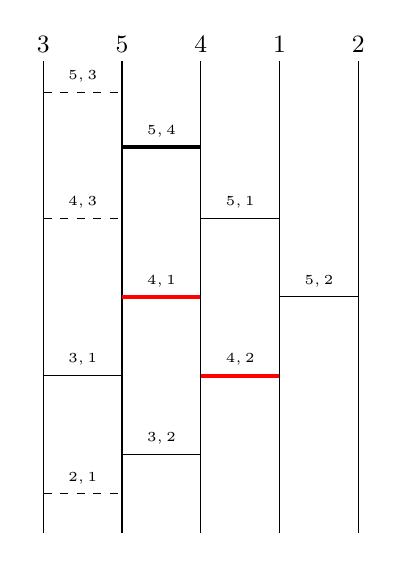
\begin{tikzpicture}
		\draw(0, 0) to (0, 6);
            \node at(.5, 5.8){\tiny{$5,3$}};
			\draw[dashed](0, 5.6) -- (1, 5.6);

            \node at(0.5, 4.2){\tiny{$4,3$}};
            \draw[dashed](0, 4) -- (1, 4);
			\node at(.5, 2.2){\tiny{$3,1$}};
			\draw(0, 2) to (1, 2);

            \draw[dashed](0, 0.5) -- (1, .5);
            \node at(.5, .7){\tiny{$2,1$}};
		\draw(1, 0) to (1, 6);
			\node at(1.5, 5.1){\tiny{$5,4$}};
			\draw[line width=.5mm](1, 4.9) to (2, 4.9);

			\node at(1.5, 3.2){\tiny{$4,1$}};
			\draw[line width=.5mm, red](1, 3.0) to (2, 3.0);

			\node at(1.5, 1.2){\tiny{$3,2$}};
			\draw(1, 1) to (2, 1);
	%		\node at(.75, .9){\tiny{$3,2$}};
	%		\draw(.5, .7) to (1, .7);
		\draw(2, 0) to (2, 6);

			\node at(2.5, 4.2){\tiny{$5,1$}};
			\draw(2, 4) to (3, 4);


			\node at(2.5, 2.2){\tiny{$4,2$}};
			\draw[line width=.5mm, red](2, 2) to (3, 2);
			%\node at(1.25, 2.1){\tiny{$4,1$}};
			%\draw[line width=.5mm, red ](1, 1.9) to (1.5, 1.9);
			%\node at(1.25, 1.3){\tiny{$5,2$}};
			%\draw(1, 1.1) to(1.5, 1.1);
		\draw(3, 0) to (3, 6);
			
			\node at(3.5, 3.2){\tiny{$5,2$}};
			\draw(3, 3.0) to (4, 3.0);	
		%\node at(1.75, 1.7){\tiny{$4,2$}};
			%\draw[line width=.5mm, red ](1.5, 1.5) to (2, 1.5);
			%\node at(1.75, .9){\tiny{$5,4$}};
			%\draw[line width=.5mm, red ](1.5, .7) to (2, .7);
		\draw(4, 0) to (4, 6);


		\node at(0.0, 6.2){\small{$3$}};
		\node at(1, 6.2){\small{$5$}};
		\node at(2.0, 6.2){\small{$4$}};
		\node at(3, 6.2){\small{$1$}};
		\node at(4, 6.2){\small{$2$}};
	\end{tikzpicture}
	\caption{The canonical ladder for $(3,5,4,1,2)$. Bars $(5,4),(4,1),(4,2)$ are part of the route of 
    $4$, but only the red bars are associated with the route of $4$.}
	\label{Fig:Route}
\end{figure}


\section{The Canonical Ladder in Detail}
In this section, we fully define the canonical ladder corresponding to $\pi$. We first define the associated terminology in order 
to provide a comprehensive definition of the canonical ladder.
Let the \emph{route} of an element be the sequence of bars the element travels along in order to reach its final position in the 
sorted permutation. The bars are read from top to bottom. In Figure~\ref{Fig:Route}, the bars $(5,4),(4,1)$ and $(4,2)$ compose the route of $4$. 
For every bar, two elements cross the bar, therefore \emph{bar association} is the association of a bar with the greater of the two elements that 
cross it. For example, in Figure~\ref{Fig:Route}, element $4$ has the bars $(5,4),(4,1)$ and 
$(4,2)$ in its route, however only bars $(4,1)$ and $(4,2)$ are associated with element $4$. Let the \emph{absence of a bar} corresponding to 
two uninverted elements in $\pi$, $x>y$, be defined as a dashed, horizontal line spanning across a column in the ladder. 
We say \emph{absence of a bar association} is the association of the absence of a bar with the greater of the two elements that form it. 
For example,$(5,3)$ are uninverted in $(3,5,4,1,2)$, therefore the absence of the bar is associated with $5$. 
For each element $2 \leq x \leq n \in \pi$, we define the \emph{associated diagonal of x} as a diagonal with $x-1$ 
row and column coordinates, having one endpoint at $(2n-2x+1, 1)$ and the other endpoint at $(2n-x-1,x-1)$.  
At each row and column in the associated diagonal of $x$, either a bar associated with $x$ or the absence of a bar associated with $x$ exists. 
For an example of the associated diagonals for the ladder corresponding to $(3,4,2,1,5)$ refer to Figure~\ref{fig:my_label}. 
\begin{figure}[h]
    \centering
    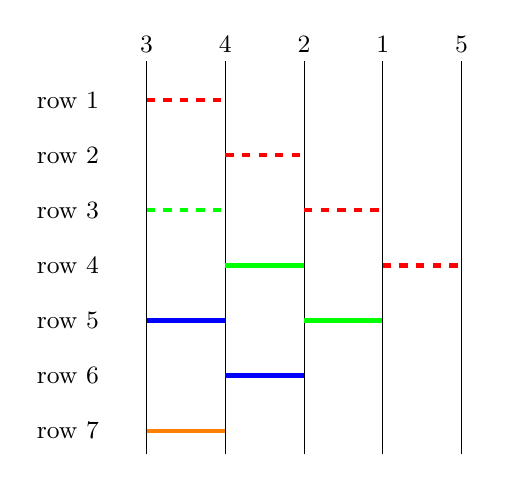
\begin{tikzpicture}
        \draw(0,0) to (0,5);
            \draw[red, dashed, line width=0.55mm](0, 4.5) -- (1,4.5);
            \draw[green, dashed, line width=0.55mm](0, 3.1) -- (1,3.1);
            \draw[blue, line width=0.55mm](0, 1.7) to (1,1.7);
            \draw[orange, line width=0.55mm](0, 0.3) to (1,0.3);

        \draw(1,0) to (1,5);
            \draw[red, dashed, line width=0.55mm](1, 3.8) -- (2,3.8);
            \draw[green, line width=0.55mm](1, 2.4) to (2,2.4);
            \draw[blue, line width=0.55mm](1, 1.0) to (2,1.0);
        \draw(2,0) to (2,5);
           \draw[red, dashed, line width=0.55mm](2, 3.1) -- (3,3.1);
            \draw[green, line width=0.55mm](2, 1.7) to (3,1.7);
        \draw(3,0) to (3,5);
         \draw[red, dashed, line width=0.55mm](3, 2.4) -- (4,2.4);
        \draw(4,0) to (4,5);

        \node at (-1, 4.5){\small{row 1}};
        \node at (-1, 3.8){\small{row 2}};
        \node at (-1, 3.1){\small{row 3}};
        \node at (-1, 2.4){\small{row 4}};
        \node at (-1, 1.7){\small{row 5}};
        \node at (-1, 1.0){\small{row 6}};
        \node at (-1, 0.3){\small{row 7}};

        \node at(0, 5.2){\small{$3$}};
        \node at(1, 5.2){\small{$4$}};
        \node at(2, 5.2){\small{$2$}};
        \node at(3, 5.2){\small{$1$}};
        \node at(4, 5.2){\small{$5$}};

    \end{tikzpicture}
    \caption{The associated diagonal of $5$ is in red, the associated diagonal of $4$ is in green, the associated diagonal of $3$ is in blue, and the associated diagonal of $2$ is in orange.}
    \label{fig:my_label}
\end{figure}

With the definition of the associated diagonal, we are now able to fully define the \emph{canonical ladder} as 
the ladder such that for each element $2 \leq x \leq n$, each bar, and absence of a bar, associated with $x$ exists 
along the associated diagonal of $x$. %Given $\pi$, we construct $CL(\pi)$ by using equation~\ref{getCordEqn} found in section 
%\textbf{Calculating the Location of a Bar for an Arbitrary $CL(\pi_{n})$}, 
%and Algorithm~\ref{Alg:RootLadder} found in section \textbf{Algorithm: Create Canonical}. 
We note that the two aforementioned figures, Figure~\ref{Fig:Route} and Figure~\ref{fig:my_label}, are the canonical ladders 
corresponding to each of their respective permutations. We use $CL(\pi)$ as shorthand notation for `the canonical ladder corresponding 
to a permutation of order $n$'. 

\section{Locating the Bar for a Given Inversion in an Arbitrary $CL(\pi)$}
In this section, we provide an equation for locating the bar in the canonical ladder associated with a given inversion, 
in an arbitrary permutation 
of order $n$. As previously stated, every bar associated with some element $x$ exists along the associated diagonal of $x$ 
within the canonical ladder. 
We use Equation~\ref{getCordEqn}, to determine the row and column for the bar corresponding 
to two elements, $x>y$, along the associated diagonal of $x$. 
Let $\pi$ be an arbitrary permutation of order $n$. Let 
$pos(x)$ be the index of $x \in \pi$. To calculate the row and column of the bar, or absence of a bar, for a pair of elements 
$x>y$, we first map $x$ to a new index termed $pos'(x)$. Let $pos'(x)$ equal $pos(x)$ minus the number of elements greater than $x$ and 
 to the left of $x$ in $\pi$. 
For example, given $\pi=(3,2,7,4,8,5,6,9,1)$, 
suppose $x=6$, then $pos'(6)=pos(6)-2=5$. 
Once we have calculated $pos'(x)$ we use a similar method to calculate $pos'(y)$. $pos'(y)$ equals 
$pos(y)$ minus the number of elements greater than $y$ and to the left of $y$ excluding $x$. For example, suppose $x$ is $7$ and 
$y$ is $5$, then $pos'(y)$ is $pos(y)-1=5$. Once we have $pos'(x)$ and $pos'(y)$, we use Equation~\ref{getCordEqn} 
to return the row and column for the bar, or absence of the bar,  
along the associated diagonal of $x$.
\begin{equation}\label{getCordEqn}
\resizebox{.9\textwidth}{!}{
\[   
    (row,column)=
    \begin{cases}
        ((2n - x - 1) - (x - pos'(y))+1,(x-1)-(x-pos'(y))+1) & \text{if $pos'(x)>pos'(y)$} \\ 
        ((2n - x - 1) - (x-pos'(y)), (x-1) - (x-pos'(y)) & \text{if $pos'(y)>pos'(x)$}
    \end{cases}
\]
}
\end{equation}

Given the inversion $(7,5) \in (3,2,7,4,8,5,6,9,1)$, we calculate the row and column of the bar $(7,5)$ using the second case. We 
get $row=(18 - 7 - 1) - (7 - 5)=8$ and $col=6-(7-5)=4$. To calculate $pos'(x)$ and $pos'(y)$, is linear amortized time. Once $pos'(x)$ 
and $pos'(y)$ are calculated,  returns the location in $O(1)$ time. 
We can use Equation~\ref{getCordEqn} to look up the location of any bar for a given $\pi$. 
In Figure~\ref{Fig:CanLArbitrary} we see $CL(3,2,7,4,8,5,6,9,1)$, where each row and column is calculated using Equation~\ref{getCordEqn}. 
\pagebreak
\begin{figure}[t]
    \centering
    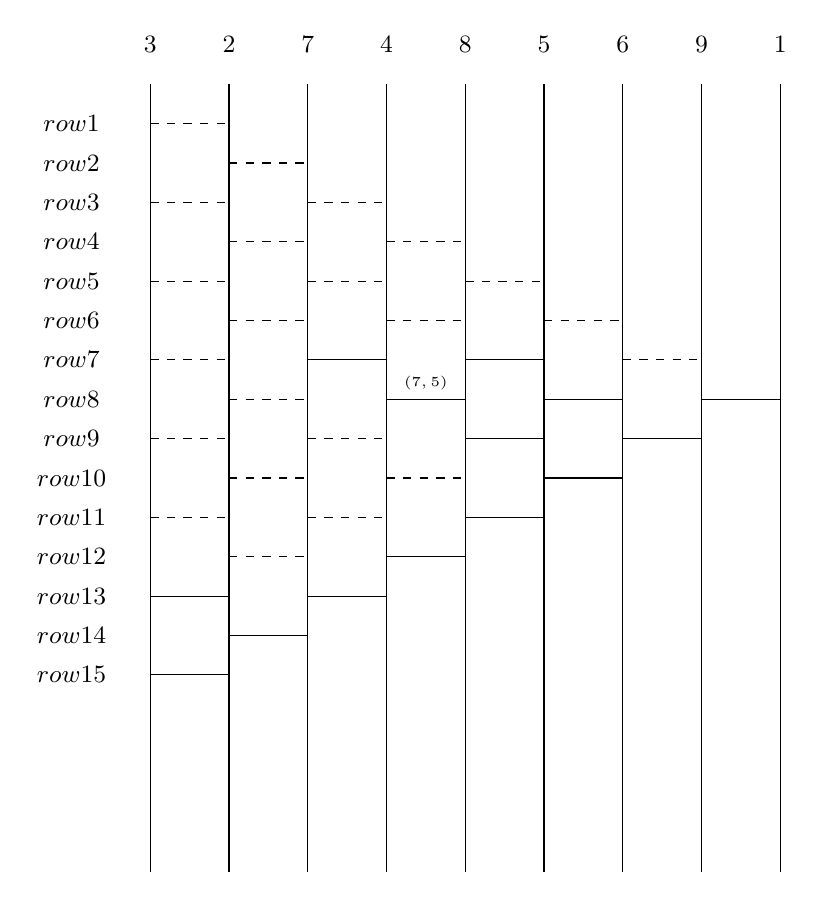
\begin{tikzpicture}
        \draw(0,0) to (0,10);
            \draw[dashed] (0, 9.5) -- (1, 9.5);
            \draw[dashed] (0, 8.5) -- (1, 8.5);
            \draw[dashed] (0, 7.5) -- (1, 7.5);
            \draw[dashed] (0, 6.5) -- (1, 6.5);
            \draw[dashed]         (0, 5.5) -- (1, 5.5);
            \draw[dashed]         (0, 4.5) -- (1, 4.5);
            \draw         (0, 3.5) to (1, 3.5);
            \draw         (0, 2.5) to (1, 2.5);
        \draw(1,0) to(1,10);
            \draw[dashed] (1, 9) -- (2, 9);
            \draw[dashed] (1, 8) -- (2, 8);
            \draw[dashed] (1, 7) -- (2, 7);
                
            \draw[dashed] (1, 6) -- (2, 6);
            \draw[dashed] (1, 5) -- (2, 5);
            \draw[dashed] (1, 4) -- (2, 4);
            \draw (1, 3) to (2, 3);
        \draw(2,0) to(2,10);
            \draw[dashed] (2, 8.5) -- (3, 8.5);
            \draw[dashed] (2, 7.5) -- (3, 7.5);
            \draw         (2, 6.5) to (3, 6.5);
            \draw[dashed] (2, 5.5) -- (3, 5.5);
            \draw[dashed] (2, 4.5) -- (3, 4.5);
            \draw         (2, 3.5) to (3, 3.5);
        \draw(3,0) to(3,10);
            \draw[dashed](3, 8) -- (4, 8);
            \draw[dashed](3, 7) -- (4, 7);
            \node at(3.5, 6.2){\tiny{$(7,5)$}};
            \draw        (3, 6) to (4, 6);
            \draw[dashed](3, 5) -- (4, 5);
            \draw        (3, 4) to (4, 4);
        \draw(4,0) to(4,10);
            \draw[dashed](4, 7.5) -- (5, 7.5);
            \draw(4, 6.5) to (5, 6.5);
            \draw(4, 5.5) to (5, 5.5);
            \draw(4, 4.5) to (5, 4.5);
        \draw(5,0) to(5,10);
            \draw[dashed](5, 7) -- (6, 7);
            \draw(5, 6) to (6, 6);
            \draw(5, 5) to (6, 5);
        \draw(6,0) to(6,10);
            \draw[dashed](6, 6.5) to (7, 6.5);
            \draw        (6, 5.5) to (7, 5.5);
        \draw(7,0) to(7,10);
            \draw(7, 6) to (8, 6);
        \draw(8,0) to(8,10);

        \node at(0, 10.5){\small{$3$}};
        \node at(1, 10.5){\small{$2$}};
        \node at(2, 10.5){\small{$7$}};
        \node at(3, 10.5){\small{$4$}};
        \node at(4, 10.5){\small{$8$}};
        \node at(5, 10.5){\small{$5$}};
        \node at(6, 10.5){\small{$6$}};
        \node at(7, 10.5){\small{$9$}};
        \node at(8, 10.5){\small{$1$}};

        \node at(-1, 9.5){\small{$row 1$}};
        \node at(-1, 9.0){\small{$row 2$}};
        \node at(-1, 8.5){\small{$row 3$}};
        \node at(-1, 8.0){\small{$row 4$}};
        \node at(-1, 7.5){\small{$row 5$}};
        \node at(-1, 7.0){\small{$row 6$}};
        \node at(-1, 6.5){\small{$row 7$}};
        \node at(-1, 6.0){\small{$row 8$}};
        \node at(-1, 5.5){\small{$row 9$}};
        \node at(-1, 5.0){\small{$row 10$}};
        \node at(-1, 4.5){\small{$row 11$}};
        \node at(-1, 4.0){\small{$row 12$}};
        \node at(-1, 3.5){\small{$row 13$}};
        \node at(-1, 3.0){\small{$row 14$}};
        \node at(-1, 2.5){\small{$row 15$}};
    \end{tikzpicture}
    \caption{Canonical ladder such that each bar or absence of a bar is calculated using the Equation~\ref{getCordEqn}.}
    \label{Fig:CanLArbitrary}
\end{figure}




\section{Locating the Bar for a Given Inversion in $CL((n,n-1, \dots 1))$}
In the previous section, we looked up a bar for a given inversion for some arbitrary permutation 
in $O(n)$ time. Clearly this is less than ideal. However, if $\pi$ is an arbitrary permutation 
of order $n$, we require linear time to calculate the location of a bar. 
In this section, we calculate the location of a bar corresponding to an inversion for $CL((n,n-1, \dots, 1))$ 
in $O(1)$ time. 
Let  $\pi=(n,n-1,n-2,...,1)$, then each associated diagonal in $CL(\pi)$ is fully occupied by bars. 
Let $x,y$ be a pair of elements in $\pi$ such that $x>y$ and $2 \leq x \leq n$. 
We know there exists a bar, $(x,y)$, in $CL((n,n-1, \dots 1))$ along the associated diagonal of $x$.
We compute the row and column of a bar $(x,y)$ in $CL((n,n-1, \dots 1))$ in $O(1)$ time using Equation~\ref{revCordEqn}. 
\begin{equation} \label{revCordEqn}
(row,column)=(2n-2x + (x-y), (x-y))
\caption{GetCoordinatesReverse}
\end{equation}

For example, given $\pi=(6,5,4,3,2,1)$, bar $(5,2)$ is located at row $5$; note that $5=(2n-2x)+(x-y)$. Bar $(5,2)$ is also located at column 
$3$; note that $3=x-y$. To see the canonical ladder for $(6,5,4,3,2,1)$ with the corresponding 
bars, please refer to Figure~\ref{Fig:RootLadderReverse}.
\begin{figure}[h]
    \centering
    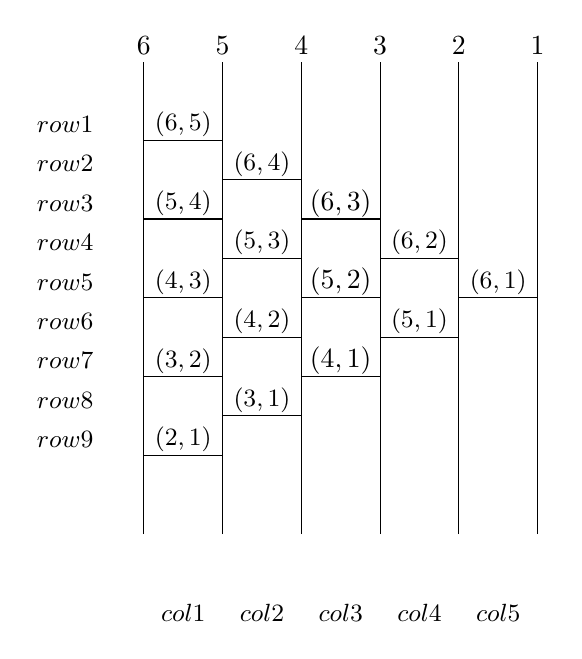
\begin{tikzpicture}
        \draw(0,0) to (0,6);
            \node at (0.5, 5.2){\small{$(6,5)$}};
            \draw(0, 5) to (1, 5);
            \node at (0.5, 4.2){\small{$(5,4)$}};
            \draw(0, 4) to (1, 4);
            \node at (0.5, 3.2){\small{$(4,3)$}};
            \draw(0, 3) to (1, 3);
            \node at (0.5, 2.2){\small{$(3,2)$}};
            \draw(0, 2) to (1, 2);
            \node at (0.5, 1.2){\small{$(2,1)$}};
            \draw(0, 1) to (1, 1);
        \draw(1,0) to (1,6);
            \node at(1.5, 4.7){\small{$(6,4)$}};
            \draw(1, 4.5) to (2, 4.5);
            \node at(1.5, 3.7){\small{$(5,3)$}};
            \draw(1, 3.5) to (2, 3.5);
            \node at(1.5, 2.7){\small{$(4,2)$}};
            \draw(1, 2.5) to (2, 2.5);
            \node at(1.5, 1.7){\small{$(3,1)$}};
            \draw(1, 1.5) to (2, 1.5);
        \draw(2,0) to (2,6);
            \node at(2.5, 4.2){$(6,3)$};
            \draw(2, 4) to (3, 4);
            \node at(2.5, 3.2){$(5,2)$};
            \draw(2, 3) to (3, 3);
            \node at(2.5, 2.2){$(4,1)$};
            \draw(2, 2) to (3, 2);
        \draw(3,0) to (3,6);
            \node at(3.5, 3.7){\small{$(6, 2)$}};
            \draw(3, 3.5) to (4, 3.5);
            \node at(3.5, 2.7){\small{$(5, 1)$}};
            \draw(3, 2.5) to (4, 2.5);
        \draw(4,0) to (4,6);
            \node at(4.5, 3.2){\small{$(6,1)$}};
            \draw(4, 3) to (5, 3);
        \draw(5,0) to (5,6);

        \node at(0, 6.2){$6$};
        \node at(1, 6.2){$5$};
        \node at(2, 6.2){$4$};
        \node at(3, 6.2){$3$};
        \node at(4, 6.2){$2$};
        \node at(5, 6.2){$1$};

        \node at(-1, 5.2){\small{$row 1$}};
        \node at(-1, 4.7){\small{$row 2$}};
        \node at(-1, 4.2){\small{$row 3$}};
        \node at(-1, 3.7){\small{$row 4$}};
        \node at(-1, 3.2){\small{$row 5$}};
        \node at(-1, 2.7){\small{$row 6$}};
        \node at(-1, 2.2){\small{$row 7$}};
        \node at(-1, 1.7){\small{$row 8$}};
        \node at(-1, 1.2){\small{$row 9$}};

        \node at(0.5, -1){\small{$col1$}};
        \node at(1.5, -1){\small{$col2$}};
        \node at(2.5, -1){\small{$col3$}};
        \node at(3.5, -1){\small{$col4$}};
        \node at(4.5, -1){\small{$col5$}};
    \end{tikzpicture}
    \caption{Canonical ladder for $(6,5,4,3,2,1)$. The location of each bar can be calculated using the formula $(2n-2x + (x-y), (x-y))$}
    \label{Fig:RootLadderReverse}
\end{figure}
We use Equation~\ref{revCordEqn} to locate a bar when we know $\pi=(n,n-1, \dots, 2,1)$. We use Equation~\ref{revCordEqn} when possible 
because the calculation time is $O(1)$ rather than $O(n)$. 


% in the corresponding $CL(\pi_{n})$. Further work is required to determine if removing bars from $CL(n,n-1, \dots, 1)$ 


\section{Algorithm: {\sc CreateCanonical}}
In this section we provide the data structure used to represent the canonical ladder in code. We then provide the algorithm for creating the canonical ladder corresponding to any permutation of 
order $n$. 
To create the canonical ladder 
we must represent the canonical ladder in code. We use Theorem~\ref{Theorem:RootHeight} and Corollary~\ref{Corollary:RootHeight} to prove the 
veracity of the representation of the canonical ladder.
 \begin{theorem}
   The number of rows required for the canonical ladder corresponding to the descending permutation of order $n$ is $2(n-1) - 1$.
   \label{Theorem:RootHeight}
 \end{theorem}
 \begin{proof}
 	Let $\pi$ be the descending permutation of order $n$. Let $route(x)$ be the route of $n \geq x \geq 2 \in \pi$. We know that 
     when $x=n$, $route(x)$ has $n-1$ bars, each requiring their own row. Thus, $CL((n,n-1, \dots, 1))$ requires at least $n-1$ rows. 
     For each subsequent $x$ from $[n-1 \dots 2]$, each $route(x)$ requires one more row to be added to $CL((n, n-1, \dots 1))$. 
     We get an additional $n-2$ rows added to $CL$, one for each $route([n-1 \geq x \geq 2])$. Therefore, the total number of rows is 
     $(n-1)+(n-2)=2(n-1)-1$.
 \end{proof}

 \begin{corollary}
     The upper bound for the number of rows of any canonical ladder of order $n$ is $2(n-1)-1$.
     \label{Corollary:RootHeight}
 \end{corollary}
 \begin{proof}
     By Theorem~\ref{Theorem:RootHeight}, we know that $2(n-1)-1$ is the number of rows required for 
     the canonical ladder corresponding 
     to the descending permutation of order $n$. By removing 
     bars from the canonical ladder for the descending permutation of order $n$, we can derive any other canonical ladder for any other permutation 
     of order $n$; removing a bar translates to removing an 
     inversion in $\pi$. Removing bars from the canonical ladder corresponding to the descending permutation of order $n$ 
     does not necessarily remove a row from the ladder, however, removing bars from the ladder certainly does not add any more rows 
     to $ladder$. Therefore, $2(n-1)-1$ is the upper bound for the number of rows required for any ladder of order $n$.
 \end{proof}
Using Theorem~\ref{Theorem:RootHeight} and Corollary~\ref{Corollary:RootHeight}, 
we represent a canonical ladder as a binary matrix with $2(n-1)-1$ rows and $n-1$ columns. Let $matrix[row][col]=1$ 
indicate a bar at the given row and column in the canonical ladder along an associated diagonal. Let $matrix[row][col]=0$ indicate the absence 
of a bar at the given row and column in the canonical ladder along an associated diagonal. Let $matrix[row][col]=-$ indicate irrelevancy as to whether 
a $1$ or $0$ is at the given row and column because the row and column do not lie on an associated diagonal. To see the canonical ladder for 
$(4,2,1,3)$ and the corresponding binary matrix, refer to Figure~\ref{Fig:MatrixLadder}.
\begin{figure}[ht]
    \begin{minipage}{.4\textwidth}
        \centering
        \begin{tikzpicture}
        \node at(0, 4.2){\small{$4$}};
        \node at(1, 4.2){\small{$2$}};
        \node at(2, 4.2){\small{$1$}};
        \node at(3, 4.2){\small{$3$}};
        \draw(0, 0) to (0, 4);
            \draw(0,3.9) to (1,3.9);
            \draw[dashed](0,1.9) -- (1,1.9);
            \draw(0,0.1) to (1,0.1);
        \draw(1, 0) to (1, 4);
            \draw(1,2.9) to (2,2.9);
            \draw[dashed](1,0.9) -- (2,0.9);
        \draw(2, 0) to (2, 4);
            \draw(2,1.9) to (3,1.9);
        \draw(3, 0) to (3, 4);
        \end{tikzpicture}
    \end{minipage}
    \begin{minipage}{0.4\textwidth}
        \begin{flushright}
        \begin{bmatrix}
            1 & - & - \\
            - & 1 & -\\
            0 & - & 1 \\ 
            - & 0 & - \\
            1 & - & - \\

        \end{bmatrix}
    \end{flushright}
    \end{minipage}
    \caption{Canonical ladder and corresponding binary matrix.}
    \label{Fig:MatrixLadder}
\end{figure}

Using Equation~\ref{getCordEqn}, and the binary matrix representation 
of a ladder, we define algorithm {\sc CreateCanonical} which can be found 
in Algorithm~\ref{Alg:RootLadder} to create the canonical ladder for 
any given permutation of order $n$. 
The initial conditions of {\sc CreateCanonical} are the 
following. Let $ladder$ be the binary matrix representing $CL(\pi)$ initialized to $-$. Let $\pi$ be an arbitrary permutation 
of order $n$. Let $x$ be the currently maximal element in $\pi$, initialized to $n$. Let {\sc GetCoordinates} refer to 
Equation~\ref{getCordEqn}. 
\begin{algorithm}[ht]
	\begin{algorithmic}[1]
		\Function {CreateCanonical}{$ladder$, $\pi$, $x$}
			\While{$x>1$}
                \State $pos(x) \gets $ index of $x \in \pi$
                \For{$i$ \textbf{from} $1$  \textbf{to} $x$}
                    \If{$i \neq pos(x)$}
                        
                        \State $(row, column) \gets${\sc GetCoordinates($x$, $pos(x), i$)}
                        \If{$pos(x)<i$}
                            \State $ladder[row][col] \gets 1$
                        \Else
                            \State $ladder[row][col] \gets 0$
                        \EndIf
                    \EndIf
                \EndFor
                \State $\pi \gets \pi - x$
                \State $x \gets x-1$
            \EndWhile
        \EndFunction

	\end{algorithmic}
	\caption{The algorithm for creating the canonical ladder of $OptL\{\pi\}$}
	\label{Alg:RootLadder}
\end{algorithm}

On each iteration of the while loop, all $x-1$ $1s$ and $0s$  along the associated diagonal of the $xth$ 
element are added to $ladder$ within the for-loop. {\sc GetCoordinates}, which refers to Equation~\ref{getCordEqn}, 
returns the row and column coordinate for the respective $1$ or $0$ for the pair of elements, $x>y$. Note that we call {\sc GetCoordinates} with 
the arguments $(x,pos(x),i)$. When referring to Equation~\ref{getCordEqn} the variables 
are $(x,pos'(x),pos'(y))$. Prior to the next iteration of the while loop, 
$x$ is removed from $\pi$ and all elements to the right of $x$ are moved to the left by one index. 
Then, $x$ is decremented by $1$. The while loop continues until $x=1$. Determining $pos(x)$ 
is done in $O(x)$ time. Removing $x$ from $\pi$ is done in $O(x)$ time. Calculating the row and column 
for each $(x,y)$ is done in $O(1)$ time. Overall, the algorithms complexity is $O(n^2)$.
We also note that {\sc CreateCanonical} creates the ladder representation with clean level $1$.  
Given three elements, $x>y>z$ and $pos(x) < pos(y) < pos(z)$, Equation~\ref{getCordEqn} returns a lesser row 
for $(x,z)$ than for $(y,z)$. Therefore, {\sc CreateCanonical} creates a representation of a ladder with clean level $1$. 
To see the resulting state of the ladder for each iteration of {\sc CreateCanonical} with $(5,7,3,4,1,2,6)$ please refer to Figure~\ref{Fig:CreateRoot}. 
\begin{figure}[t]
    \centering 
    \begin{minipage}{.3\textwidth}
    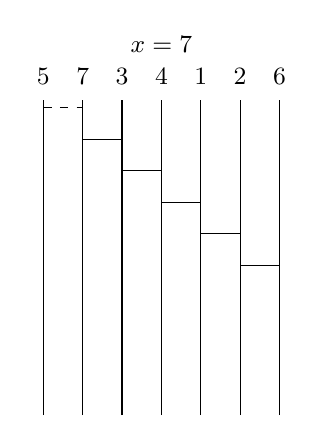
\begin{tikzpicture}
        \draw(0, 0) to (0, 4);
        
        \draw(.5, 0) to (.5, 4);
        \draw(1, 0) to (1, 4);
        \draw(1.5, 0) to (1.5, 4);
        \draw(2, 0) to (2, 4);
        \draw(2.5, 0) to (2.5, 4);
        \draw(3, 0) to (3, 4);
        
        \draw(2.5, 1.9) to (3, 1.9);
        \draw(2.0, 2.3) to (2.5, 2.3);
        \draw(1.5, 2.7) to (2.0, 2.7);
        \draw(1.0, 3.1) to (1.5, 3.1);
        \draw(0.5, 3.5) to (1.0, 3.5);

        \draw[dashed] (0, 3.9) -- (0.5, 3.9);
        \node at(1.5, 4.7){\small{$x=7$}};
        \node at(0, 4.3){\small{$5$}};
        \node at(.5, 4.3){\small{$7$}};
        \node at(1, 4.3){\small{$3$}};
        \node at(1.5, 4.3){\small{$4$}};
        \node at(2, 4.3){\small{$1$}};
        \node at(2.5, 4.3){\small{$2$}};
        \node at(3, 4.3){\small{$6$}};
    \end{tikzpicture}
    \end{minipage}
    \begin{minipage}{.3\textwidth}
    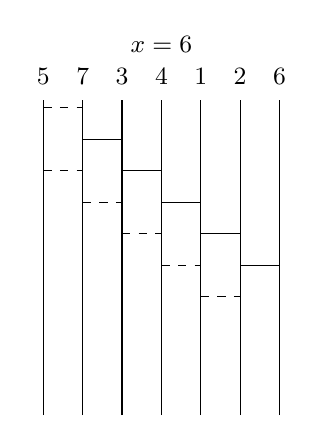
\begin{tikzpicture}
        \draw(0, 0) to (0, 4);
        \draw(.5, 0) to (.5, 4);
        \draw(1, 0) to (1, 4);
        \draw(1.5, 0) to (1.5, 4);
        \draw(2, 0) to (2, 4);
        \draw(2.5, 0) to (2.5, 4);
        \draw(3, 0) to (3, 4);
        
        \draw[dashed] (0, 3.9) -- (0.5, 3.9);
        \draw[dashed] (2, 1.5) -- (2.5, 1.5);
        \draw[dashed] (1.5, 1.9) -- (2.0, 1.9);
        \draw[dashed] (1.0, 2.3) -- (1.5, 2.3);
        \draw[dashed] (0.5, 2.7) -- (1.0, 2.7);
        \draw[dashed] (0.0, 3.1) -- (0.5, 3.1);
        \draw(2.5, 1.9) to (3, 1.9);
        \draw(2.0, 2.3) to (2.5, 2.3);
        \draw(1.5, 2.7) to (2.0, 2.7);
        \draw(1.0, 3.1) to (1.5, 3.1);
        \draw(0.5, 3.5) to (1.0, 3.5);

        \node at(1.5, 4.7){\small{$x=6$}};

        \node at(0, 4.3){\small{$5$}};
        \node at(.5, 4.3){\small{$7$}};
        \node at(1, 4.3){\small{$3$}};
        \node at(1.5, 4.3){\small{$4$}};
        \node at(2, 4.3){\small{$1$}};
        \node at(2.5, 4.3){\small{$2$}};
        \node at(3, 4.3){\small{$6$}};
    \end{tikzpicture}
    \end{minipage}
   \begin{minipage}{.3\textwidth}
    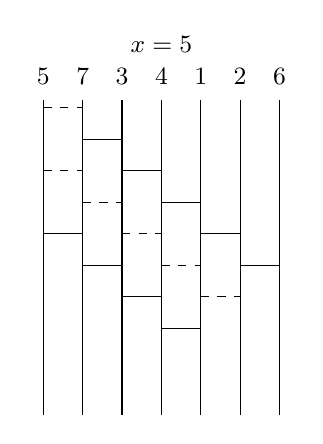
\begin{tikzpicture}
        \draw(0, 0) to (0, 4);
            \draw(0, 2.3) to (0.5, 2.3);
        \draw(.5, 0) to (.5, 4);
            \draw(.5, 1.9) to (1, 1.9);
        \draw(1, 0) to (1, 4);
            \draw(1, 1.5) to (1.5, 1.5);
        \draw(1.5, 0) to (1.5, 4);
            \draw(1.5, 1.1) to (2, 1.1);
            \draw(1.5, 2.7) to (2, 2.7);
        \draw(2, 0) to (2, 4);
        \draw(2.5, 0) to (2.5, 4);
        \draw(3, 0) to (3, 4);
      


        \draw(2.5, 1.9) to (3, 1.9);
        \draw(2.0, 2.3) to (2.5, 2.3);

        \draw(1.0, 3.1) to (1.5, 3.1);
        \draw(0.5, 3.5) to (1.0, 3.5);
      
        \draw[dashed] (0, 3.9) -- (0.5, 3.9);
        \draw[dashed] (2, 1.5) -- (2.5, 1.5);
        \draw[dashed] (1.5, 1.9) -- (2.0, 1.9);
        \draw[dashed] (1.0, 2.3) -- (1.5, 2.3);
        \draw[dashed] (0.5, 2.7) -- (1.0, 2.7);
        \draw[dashed] (0.0, 3.1) -- (0.5, 3.1);
        

        \node at(1.5, 4.7){\small{$x=5$}};
        \node at(0, 4.3){\small{$5$}};
        \node at(.5, 4.3){\small{$7$}};
        \node at(1, 4.3){\small{$3$}};
        \node at(1.5, 4.3){\small{$4$}};
        \node at(2, 4.3){\small{$1$}};
        \node at(2.5, 4.3){\small{$2$}};
        \node at(3, 4.3){\small{$6$}};
    \end{tikzpicture}
    \end{minipage}
        
    \begin{minipage}{.3\textwidth}
    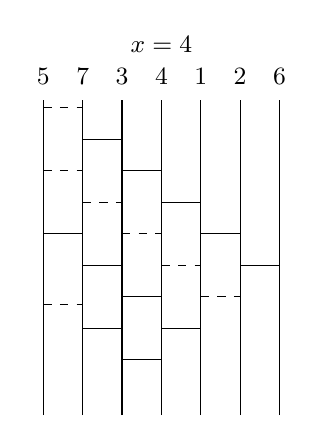
\begin{tikzpicture}
    \draw(0, 0) to (0, 4);
            \draw(0, 2.3) to (0.5, 2.3);
        \draw(.5, 0) to (.5, 4);
            \draw(.5, 1.9) to (1, 1.9);
            \draw(0.5, 1.1) to (1, 1.1);
        \draw(1, 0) to (1, 4);
            \draw(1, 1.5) to (1.5, 1.5);
            \draw(1, 0.7) to (1.5, 0.7);
        \draw(1.5, 0) to (1.5, 4);
            \draw(1.5, 1.1) to (2, 1.1);
            \draw(1.5, 2.7) to (2, 2.7);
        \draw(2, 0) to (2, 4);
        \draw(2.5, 0) to (2.5, 4);
        \draw(3, 0) to (3, 4);
        

        \draw(2.5, 1.9) to (3, 1.9);
        \draw(2.0, 2.3) to (2.5, 2.3);

        \draw(1.0, 3.1) to (1.5, 3.1);
        \draw(0.5, 3.5) to (1.0, 3.5);
      
        \draw[dashed] (0, 3.9) -- (0.5, 3.9);
        \draw[dashed] (2, 1.5) -- (2.5, 1.5);
        \draw[dashed] (1.5, 1.9) -- (2.0, 1.9);
        \draw[dashed] (1.0, 2.3) -- (1.5, 2.3);
        \draw[dashed] (0.5, 2.7) -- (1.0, 2.7);
        \draw[dashed] (0.0, 3.1) -- (0.5, 3.1);
        \draw[dashed] (0.0, 1.4) -- (0.5, 1.4);
        

        \node at(1.5, 4.7){\small{$x=4$}};
        \node at(0, 4.3){\small{$5$}};
        \node at(.5, 4.3){\small{$7$}};
        \node at(1, 4.3){\small{$3$}};
        \node at(1.5, 4.3){\small{$4$}};
        \node at(2, 4.3){\small{$1$}};
        \node at(2.5, 4.3){\small{$2$}};
        \node at(3, 4.3){\small{$6$}};
    \end{tikzpicture}
    \end{minipage}
    \begin{minipage}{.3\textwidth}
    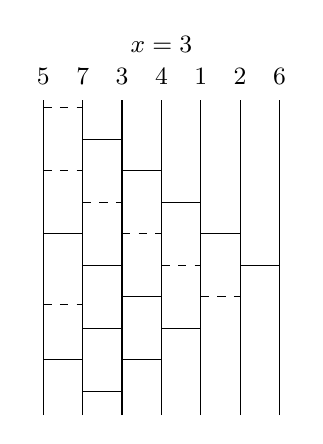
\begin{tikzpicture}
     \draw(0, 0) to (0, 4);
            \draw(0, 2.3) to (0.5, 2.3);
            \draw(0, 0.7) to (0.5, 0.7);
        \draw(.5, 0) to (.5, 4);
            \draw(.5, 1.9) to (1, 1.9);
            \draw(0.5, 1.1) to (1, 1.1);
            \draw(0.5, 0.3) to (1, 0.3);
        \draw(1, 0) to (1, 4);
            \draw(1, 1.5) to (1.5, 1.5);
            \draw(1, 0.7) to (1.5, 0.7);
        \draw(1.5, 0) to (1.5, 4);
            \draw(1.5, 1.1) to (2, 1.1);
            \draw(1.5, 2.7) to (2, 2.7);
        \draw(2, 0) to (2, 4);
        \draw(2.5, 0) to (2.5, 4);
        \draw(3, 0) to (3, 4);
       

        \draw(2.5, 1.9) to (3, 1.9);
        \draw(2.0, 2.3) to (2.5, 2.3);

        \draw(1.0, 3.1) to (1.5, 3.1);
        \draw(0.5, 3.5) to (1.0, 3.5);
      
        \draw[dashed] (0, 3.9) -- (0.5, 3.9);
        \draw[dashed] (2, 1.5) -- (2.5, 1.5);
        \draw[dashed] (1.5, 1.9) -- (2.0, 1.9);
        \draw[dashed] (1.0, 2.3) -- (1.5, 2.3);
        \draw[dashed] (0.5, 2.7) -- (1.0, 2.7);
        \draw[dashed] (0.0, 3.1) -- (0.5, 3.1);
        \draw[dashed] (0.0, 1.4) -- (0.5, 1.4);
        

        \node at(1.5, 4.7){\small{$x=3$}};
        \node at(0, 4.3){\small{$5$}};
        \node at(.5, 4.3){\small{$7$}};
        \node at(1, 4.3){\small{$3$}};
        \node at(1.5, 4.3){\small{$4$}};
        \node at(2, 4.3){\small{$1$}};
        \node at(2.5, 4.3){\small{$2$}};
        \node at(3, 4.3){\small{$6$}};
    \end{tikzpicture}
    \end{minipage}
    \begin{minipage}{.3\textwidth}
   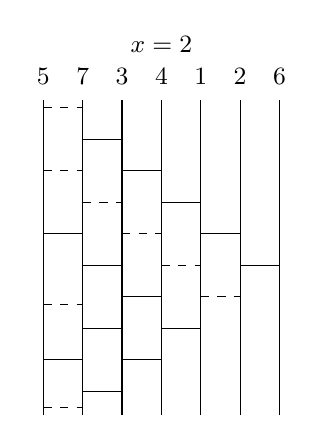
\begin{tikzpicture}
     \draw(0, 0) to (0, 4);
            \draw(0, 2.3) to (0.5, 2.3);
            \draw(0, 0.7) to (0.5, 0.7);
        \draw(.5, 0) to (.5, 4);
            \draw(.5, 1.9) to (1, 1.9);
            \draw(0.5, 1.1) to (1, 1.1);
            \draw(0.5, 0.3) to (1, 0.3);
        \draw(1, 0) to (1, 4);
            \draw(1, 1.5) to (1.5, 1.5);
            \draw(1, 0.7) to (1.5, 0.7);
        \draw(1.5, 0) to (1.5, 4);
            \draw(1.5, 1.1) to (2, 1.1);
            \draw(1.5, 2.7) to (2, 2.7);
        \draw(2, 0) to (2, 4);
        \draw(2.5, 0) to (2.5, 4);
        \draw(3, 0) to (3, 4);
      


        \draw(2.5, 1.9) to (3, 1.9);
        \draw(2.0, 2.3) to (2.5, 2.3);

        \draw(1.0, 3.1) to (1.5, 3.1);
        \draw(0.5, 3.5) to (1.0, 3.5);
      
        \draw[dashed] (0, 3.9) -- (0.5, 3.9);
        \draw[dashed] (2, 1.5) -- (2.5, 1.5);
        \draw[dashed] (1.5, 1.9) -- (2.0, 1.9);
        \draw[dashed] (1.0, 2.3) -- (1.5, 2.3);
        \draw[dashed] (0.5, 2.7) -- (1.0, 2.7);
        \draw[dashed] (0.0, 3.1) -- (0.5, 3.1);
        \draw[dashed] (0.0, 1.4) -- (0.5, 1.4);
        \draw[dashed] (0.0, 0.1) -- (0.5,0.1);
        

        \node at(1.5, 4.7){\small{$x=2$}};
        \node at(0, 4.3){\small{$5$}};
        \node at(.5, 4.3){\small{$7$}};
        \node at(1, 4.3){\small{$3$}};
        \node at(1.5, 4.3){\small{$4$}};
        \node at(2, 4.3){\small{$1$}};
        \node at(2.5, 4.3){\small{$2$}};
        \node at(3, 4.3){\small{$6$}};

    \end{tikzpicture}
    \end{minipage}
    

        
        % \node at(9.5, -5.3){\small{$x=2,row=10$}};

        % \node at(0, -.7){\small{$5$}};
        % \node at(.5, -.7){\small{$7$}};
        % \node at(1, -.7){\small{$3$}};
        % \node at(1.5, -.7){\small{$4$}};
        % \node at(2, -.7){\small{$1$}};
        % \node at(2.5, -.7){\small{$2$}};
        % \node at(3, -.7){\small{$6$}};
        
        % \node at(4, -.7){\small{$5$}};
        % \node at(4.5, -.7){\small{$7$}};
        % \node at(5, -.7){\small{$3$}};
        % \node at(5.5, -.7){\small{$4$}};
        % \node at(6, -.7){\small{$1$}};
        % \node at(6.5, -.7){\small{$2$}};
        % \node at(7, -.7){\small{$6$}};

        % \node at(8, -.7){\small{$5$}};
        % \node at(8.5, -.7){\small{$7$}};
        % \node at(9, -.7){\small{$3$}};
        % \node at(9.5, -.7){\small{$4$}};
        % \node at(10, -.7){\small{$1$}};
        % \node at(10.5, -.7){\small{$2$}};
        % \node at(11, -.7){\small{$6$}};
        
    
    \caption{The ordering of the state of the ladder when creating the root ladder for $(5,7,3,4,1,2,6)$}
    \label{Fig:CreateRoot}
\end{figure}

% \begin{lemma}
% 	The time complexity for CreateRoot is $O(n^{2})$
% \end{lemma}
% \begin{proof}
% 	The for-loop runs from some arbitrary index to $n$ on each function call. Thus, we get $O(n)$. The following 
%     recursion holds, $CreateRoot(n-k) = CreateRoot((n-k)+1) + n=CreateRoot((n-k)+2) + n-1\dots $. The recurrence 
%     relation is reduced to $n(n+1)/2= O(n^2)$.
% \end{proof}

A main contribution of this thesis is the canonical ladder and the algorithm {\sc CreateCanonical}.
By defining the canonical ladder we are able to list all $n!$ canonical ladders in any order. 
Let $L_{n}$ be the set of all $n!$ canonical ladders. 
\begin{lemma}
    Using {\sc CreateCanonical}, we can list $L_{n}$ in any order.
\end{lemma}
\begin{proof}
 Let $S_{n}$ be the set of all permutations of order $n$. We simply apply an ordering to list $S_{n}$. For each 
 permutation in $S_{n}$, we apply {\sc CreateCanonical}, thus listing $L_{n}$ in the same order as $S_{n}$.
\end{proof}
We create each $CL(\pi)$ in $O(n^2)$ time using {\sc CreateCanonical}. However, using {\sc CreateCanonical} to list $L_{n}$ is inefficient, 
seeing as each ladder is created in $O(n^2)$ time. 
In chapters 4 and 5 we provide two Gray code listing algorithms, {\sc ModifiedSJT} and {\sc ListLnByKBars}, to list $L_{n}$ in constant amortized time. 
The details of these algorithms are found in chapters 4 and 5 respectively.  
% {\sc ModifiedSJT} and {\sc CyclicBar} require additional auxiliary functions. We define {\sc Inv(x)} as follows: $|\forall y \in \pi : y < x, p_{y}>p_{x}|$. 
% For example, given $(3,4,1,5,6,2)$, {\sc Inv(1)=0}, {\sc Inv(2)=0}, {\sc Inv(3)=2}, {\sc Inv(4)=2}, {\sc Inv(5)=1}, {\sc Inv(6)=1}. 
% Given {\sc Inv(x)}, 
% we can define the function {\sc GetCoordinates2}. In order to define {\sc GetCoordinates2}, let $x>y \in \pi$. Given 
% $p_{x}$ and $p_{y}$, suppose a transposition were applied to $x$ and $y$. Prior to the transposition 
% of $x$ and $y$, if $p_{x} = p_{y}-1$ then {\sc GetCoordinates2} returns the row and column of the bar $(x,y)$ to be removed 
% from the ladder. If $p_{x}=p_{y}+1$, then {\sc GetCoordinates} returns 
% the row and column of bar $(x,y)$ to be added to the ladder. 








\section{Procedure}

So far, the problem has been introduced and the required terminology has been defined. In the procedure section,
 the details of {\sc ModifiedSJT} and {\sc CyclicBar} are provided. These details include the pseudocode for 
 each of the algorithms, the initial conditions for each of the algorithms, the structures produced by each 
 of the algorithms, and a number of lemmas and proofs for each of the two algorithms. In the procedure section, 
 the algorithms are assessed independently of each other.
%%section SJT
\subsection{The Modified Steinhaus-Johnson-Trotter Algorithm}

For the initial conditions of {\sc ModifiedSJT} assume the following. 
Let be the $ladder$ be initialized a two dimensional binary array of only $0's$.
 Let a $1$ at $row=i,col=j$ 
indicate a bar at  $row=i,col=j$. Let a $0$ at $row=i,col=j$ 
indicate the absence of a bar at  $row=i,col=j$.
Let $n$ be the maximum element. Let $direction$ be a one 
indexed array set to left for all indexes. Let left indicate that a bar is to be added to the ladder; bars 
are added left to right. Let right indicate a bar is to be removed from the ladder; bars 
are removed right to left. Let $route$ be initialized to $2$. On each recursive call 
$route$ is incremented by $1$ from $2,3 \dots n$.
\begin{algorithm}
  \begin{algorithmic}[1]
    \Function{ModifiedSJT}{$n$, $ladder$, $route$, $direction$}
     %%base case
      \If{$route > n$}
        \State {\sc print}($ladder$)
        \State \textbf{return}
      \EndIf
      %%swap the nth element n-1 times
      \For{$i$ \textbf{from} $0$ \textbf{to} $route-1$}
        \If{$i = 0$}
          \State {\sc ModifiedSJT}($n$, $ladder$, $route+1$, $direction$)
        \Else 
          \If{$direction[route]=$ left}
            \State $row \gets (n) + (n - route) - (i);$
            \State $col \gets route - i$
            \State $ladder[row][col] \gets 1$
          \Else
            \State $col \gets i$
            \State $row \gets 2(n - route) + (i)$
            \State $ladder[row][col] \gets 0$
          \EndIf
        \EndIf
        \State {\sc ModifiedSJT}($n$, $ladder$, $route+1$, $direction$)
      \EndFor
      \If{$direction[route] =$ left}
        \State $direction[route] \gets$ right
      \Else
        \State $direction[route] \gets$ left
      \EndIf
    \EndFunction
  \end{algorithmic}
  \caption{Modification of the {\sc SJT} algorithm for listing $L_{n}$}
  \label{Alg:ModSJT}
\end{algorithm}


\pagebreak


The principles of the algorithm are the following. Given $route=k$, add or remove a bar for route $k$, then add or remove 
all bars for $route=k+1$. Once all bars for route $k+1$ have been added or removed, 
proceed to add or remove the next bar from $route=k$. Repeat until all $k-1$ bars have been added or removed from route $k$.
If $direction[route]$ is left, then bars of $route$ will be added to 
$ladder$ from right to left, bottom to top, until no more bars to $route$ can be added.
If $direction[route]$ is right, then bars will be removed from $ladder$, right to left, top to bottom, until 
no more bars from $route$ can be removed. Once all the bars for $route$ have 
been added or removed, then $direction[route]$ is reversed,
indicating that the opposite operation will be applied to the bars of the route when 
$route$ is next processed. The maximum number of bars for a given $route=k$ is $k-1$ and the minimum number of 
bars is $1$. On each recursive call, $route$ is 
incremented by $1$. When $route$ is greater than $n$, print the ladder 
and return. 


\begin{lemma}
  {\sc ModifiedSJT} produces $L_{n}$
\end{lemma}
\begin{proof}
  Since the algorithm is a modification of the Steinhaus-Johnson-Trotter algorithm, a similar proof for the SJT algorithm 
can be applied to the {\sc ModifiedSJT} algorithm. Suppose we want to list all $n!$ ladders 
of order $n$. Suppose we have all $n-1!$ ladders of order $n-1$, then for 
each ladder of order $n-1$ add a new column to the right; this results in $n-1$ columns seeing as 
the number of columns is one less than the number of elements. For each of the $n-1!$ ladders with $n-1$ columns 
add $0 \dots n-1$ bars beginning at column $n-1$ and ending 
at column $1$. Doing so results in $(n-1)!n=n!$ ladders of order $n$. To see 
an example of the proof please refer to Figure~\ref{Fig:CanLSJT}.
\end{proof}
%%prove the dimensions of the datastructure
\begin{center}
 \begin{figure}[!htp]
  \centering
  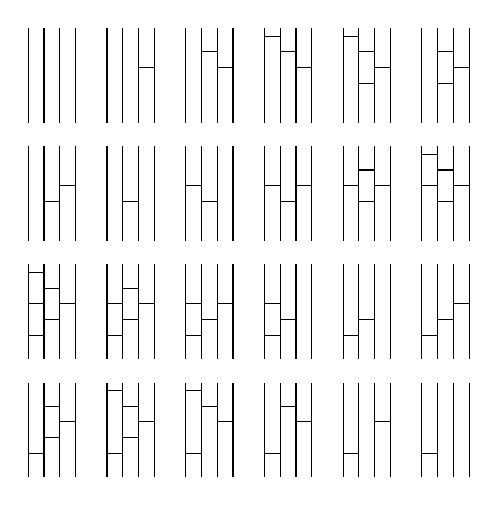
\begin{tikzpicture}
\draw(0.00,5.90) to (0.00,7.10);
\draw(0.20,5.90) to (0.20,7.10);
\draw(0.40,5.90) to (0.40,7.10);
\draw(0.60,5.90) to (0.60,7.10);


\draw(1.00,5.90) to (1.00,7.10);
\draw(1.20,5.90) to (1.20,7.10);
\draw(1.40,5.90) to (1.40,7.10);
\draw(1.60,5.90) to (1.60,7.10);
\draw(1.40, 6.60) to (1.60, 6.60);


\draw(2.00,5.90) to (2.00,7.10);
\draw(2.20,5.90) to (2.20,7.10);
\draw(2.40,5.90) to (2.40,7.10);
\draw(2.60,5.90) to (2.60,7.10);
\draw(2.20, 6.80) to (2.40, 6.80);
\draw(2.40, 6.60) to (2.60, 6.60);


\draw(3.00,5.90) to (3.00,7.10);
\draw(3.20,5.90) to (3.20,7.10);
\draw(3.40,5.90) to (3.40,7.10);
\draw(3.60,5.90) to (3.60,7.10);
\draw(3.00, 7.00) to (3.20, 7.00);
\draw(3.20, 6.80) to (3.40, 6.80);
\draw(3.40, 6.60) to (3.60, 6.60);


\draw(4.00,5.90) to (4.00,7.10);
\draw(4.20,5.90) to (4.20,7.10);
\draw(4.40,5.90) to (4.40,7.10);
\draw(4.60,5.90) to (4.60,7.10);
\draw(4.00, 7.00) to (4.20, 7.00);
\draw(4.20, 6.80) to (4.40, 6.80);
\draw(4.40, 6.60) to (4.60, 6.60);
\draw(4.20, 6.40) to (4.40, 6.40);


\draw(5.00,5.90) to (5.00,7.10);
\draw(5.20,5.90) to (5.20,7.10);
\draw(5.40,5.90) to (5.40,7.10);
\draw(5.60,5.90) to (5.60,7.10);
\draw(5.20, 6.80) to (5.40, 6.80);
\draw(5.40, 6.60) to (5.60, 6.60);
\draw(5.20, 6.40) to (5.40, 6.40);


\draw(0.00,4.40) to (0.00,5.60);
\draw(0.20,4.40) to (0.20,5.60);
\draw(0.40,4.40) to (0.40,5.60);
\draw(0.60,4.40) to (0.60,5.60);
\draw(0.40, 5.10) to (0.60, 5.10);
\draw(0.20, 4.90) to (0.40, 4.90);


\draw(1.00,4.40) to (1.00,5.60);
\draw(1.20,4.40) to (1.20,5.60);
\draw(1.40,4.40) to (1.40,5.60);
\draw(1.60,4.40) to (1.60,5.60);
\draw(1.20, 4.90) to (1.40, 4.90);


\draw(2.00,4.40) to (2.00,5.60);
\draw(2.20,4.40) to (2.20,5.60);
\draw(2.40,4.40) to (2.40,5.60);
\draw(2.60,4.40) to (2.60,5.60);
\draw(2.00, 5.10) to (2.20, 5.10);
\draw(2.20, 4.90) to (2.40, 4.90);


\draw(3.00,4.40) to (3.00,5.60);
\draw(3.20,4.40) to (3.20,5.60);
\draw(3.40,4.40) to (3.40,5.60);
\draw(3.60,4.40) to (3.60,5.60);
\draw(3.00, 5.10) to (3.20, 5.10);
\draw(3.40, 5.10) to (3.60, 5.10);
\draw(3.20, 4.90) to (3.40, 4.90);


\draw(4.00,4.40) to (4.00,5.60);
\draw(4.20,4.40) to (4.20,5.60);
\draw(4.40,4.40) to (4.40,5.60);
\draw(4.60,4.40) to (4.60,5.60);
\draw(4.20, 5.30) to (4.40, 5.30);
\draw(4.00, 5.10) to (4.20, 5.10);
\draw(4.40, 5.10) to (4.60, 5.10);
\draw(4.20, 4.90) to (4.40, 4.90);


\draw(5.00,4.40) to (5.00,5.60);
\draw(5.20,4.40) to (5.20,5.60);
\draw(5.40,4.40) to (5.40,5.60);
\draw(5.60,4.40) to (5.60,5.60);
\draw(5.00, 5.50) to (5.20, 5.50);
\draw(5.20, 5.30) to (5.40, 5.30);
\draw(5.00, 5.10) to (5.20, 5.10);
\draw(5.40, 5.10) to (5.60, 5.10);
\draw(5.20, 4.90) to (5.40, 4.90);


\draw(0.00,2.90) to (0.00,4.10);
\draw(0.20,2.90) to (0.20,4.10);
\draw(0.40,2.90) to (0.40,4.10);
\draw(0.60,2.90) to (0.60,4.10);
\draw(0.00, 4.00) to (0.20, 4.00);
\draw(0.20, 3.80) to (0.40, 3.80);
\draw(0.00, 3.60) to (0.20, 3.60);
\draw(0.40, 3.60) to (0.60, 3.60);
\draw(0.20, 3.40) to (0.40, 3.40);
\draw(0.00, 3.20) to (0.20, 3.20);


\draw(1.00,2.90) to (1.00,4.10);
\draw(1.20,2.90) to (1.20,4.10);
\draw(1.40,2.90) to (1.40,4.10);
\draw(1.60,2.90) to (1.60,4.10);
\draw(1.20, 3.80) to (1.40, 3.80);
\draw(1.00, 3.60) to (1.20, 3.60);
\draw(1.40, 3.60) to (1.60, 3.60);
\draw(1.20, 3.40) to (1.40, 3.40);
\draw(1.00, 3.20) to (1.20, 3.20);


\draw(2.00,2.90) to (2.00,4.10);
\draw(2.20,2.90) to (2.20,4.10);
\draw(2.40,2.90) to (2.40,4.10);
\draw(2.60,2.90) to (2.60,4.10);
\draw(2.00, 3.60) to (2.20, 3.60);
\draw(2.40, 3.60) to (2.60, 3.60);
\draw(2.20, 3.40) to (2.40, 3.40);
\draw(2.00, 3.20) to (2.20, 3.20);


\draw(3.00,2.90) to (3.00,4.10);
\draw(3.20,2.90) to (3.20,4.10);
\draw(3.40,2.90) to (3.40,4.10);
\draw(3.60,2.90) to (3.60,4.10);
\draw(3.00, 3.60) to (3.20, 3.60);
\draw(3.20, 3.40) to (3.40, 3.40);
\draw(3.00, 3.20) to (3.20, 3.20);


\draw(4.00,2.90) to (4.00,4.10);
\draw(4.20,2.90) to (4.20,4.10);
\draw(4.40,2.90) to (4.40,4.10);
\draw(4.60,2.90) to (4.60,4.10);
\draw(4.20, 3.40) to (4.40, 3.40);
\draw(4.00, 3.20) to (4.20, 3.20);


\draw(5.00,2.90) to (5.00,4.10);
\draw(5.20,2.90) to (5.20,4.10);
\draw(5.40,2.90) to (5.40,4.10);
\draw(5.60,2.90) to (5.60,4.10);
\draw(5.40, 3.60) to (5.60, 3.60);
\draw(5.20, 3.40) to (5.40, 3.40);
\draw(5.00, 3.20) to (5.20, 3.20);


\draw(0.00,1.40) to (0.00,2.60);
\draw(0.20,1.40) to (0.20,2.60);
\draw(0.40,1.40) to (0.40,2.60);
\draw(0.60,1.40) to (0.60,2.60);
\draw(0.20, 2.30) to (0.40, 2.30);
\draw(0.40, 2.10) to (0.60, 2.10);
\draw(0.20, 1.90) to (0.40, 1.90);
\draw(0.00, 1.70) to (0.20, 1.70);


\draw(1.00,1.40) to (1.00,2.60);
\draw(1.20,1.40) to (1.20,2.60);
\draw(1.40,1.40) to (1.40,2.60);
\draw(1.60,1.40) to (1.60,2.60);
\draw(1.00, 2.50) to (1.20, 2.50);
\draw(1.20, 2.30) to (1.40, 2.30);
\draw(1.40, 2.10) to (1.60, 2.10);
\draw(1.20, 1.90) to (1.40, 1.90);
\draw(1.00, 1.70) to (1.20, 1.70);


\draw(2.00,1.40) to (2.00,2.60);
\draw(2.20,1.40) to (2.20,2.60);
\draw(2.40,1.40) to (2.40,2.60);
\draw(2.60,1.40) to (2.60,2.60);
\draw(2.00, 2.50) to (2.20, 2.50);
\draw(2.20, 2.30) to (2.40, 2.30);
\draw(2.40, 2.10) to (2.60, 2.10);
\draw(2.00, 1.70) to (2.20, 1.70);


\draw(3.00,1.40) to (3.00,2.60);
\draw(3.20,1.40) to (3.20,2.60);
\draw(3.40,1.40) to (3.40,2.60);
\draw(3.60,1.40) to (3.60,2.60);
\draw(3.20, 2.30) to (3.40, 2.30);
\draw(3.40, 2.10) to (3.60, 2.10);
\draw(3.00, 1.70) to (3.20, 1.70);


\draw(4.00,1.40) to (4.00,2.60);
\draw(4.20,1.40) to (4.20,2.60);
\draw(4.40,1.40) to (4.40,2.60);
\draw(4.60,1.40) to (4.60,2.60);
\draw(4.40, 2.10) to (4.60, 2.10);
\draw(4.00, 1.70) to (4.20, 1.70);


\draw(5.00,1.40) to (5.00,2.60);
\draw(5.20,1.40) to (5.20,2.60);
\draw(5.40,1.40) to (5.40,2.60);
\draw(5.60,1.40) to (5.60,2.60);
\draw(5.00, 1.70) to (5.20, 1.70);






\end{tikzpicture}
  \caption{$L_{4}$ generated by the {\sc ModifiedSJT} algorithm. The algorithm inserts or removes a bar between any two successive ladders.}
  \label{Fig:CanLSJT}
\end{figure}
\end{center}\pagebreak

\begin{theorem}
  If the algorithm being applied is {\sc ModifiedSJT} then the number of rows required for the ladder data-structure is $2(n-1) - 1$ 
  and the number of columns required for the ladder is $n-1$.
\end{theorem}
\begin{proof}
  The number of columns is fairly straightforward. Seeing as there are always $n$ elements in $\pi_{n}$, 
  a column represents a gap between lines in the corresponding ladder lottery. Each ladder of order $n$ has $n$ lines, 
  one for each element in $\pi_{n}$. Therefore each ladder of order $n$ has $n-1$ columns.\par 
  The number of rows for the ladder data-structure is calculated a follows, given $\pi_{n}$, the minimal 
  number of rows required is when $\pi_{n}$ is sorted. In this case there are zero rows because there are 
  zero bars added to the ladder. When a bar is added to the ladder it can be added to an already existing row 
  or to a new row. If the current state of the ladder is empty then adding the first bar produces the second ladder in
  $L_{n}$. Since the bars are being added bottom right to top left, and the first bar to be added belongs 
  to the $nth$ route, then it must be added to $row=n-1$, $col=n-1$. As bars of the $nth$ route get 
  continuously added to the ladder, each bar is added a row above the previous bar and to a column 
  to the left of the column of the previous bar.
  Since no two bars of the $nth$ route can be on the same row, this will require $n-1$ rows. Note, if they were added to the same 
  row, then the left end point of the right bar would be touching the right end point of the left bar which is disallowed. Once the 
  bars of the $nth$ element are added, the bars of the $n-1th$ route will be added. The $n-1th's$ first bar 
  will be added to the $n-2$ column, otherwise it would be directly below the first bar of the $nth$ route, which is a violation. 
  Since the first bar of the $n-1$'s element is added to column $n-2$, then it must be given a new row, otherwise its right end point 
  will be touching  the left end point of the first bar of route $n$. The remaining $n-2$ bars of element $n-1$
  will be added bottom right to top left, but none of their end points will touch the end points of element $n$ seeing as they will 
  always be two columns apart from any bar in $n's$ route. The same logic applies to element $n-2$, it will require one extra row for its 
  first bar, in order not to touch the first bar of element $n-1$, but the remainder of its bars will always be two columns away from 
  the remainder of the bars for $n-1$, etc. Therefore there are $n-1$ rows required for the $nth$ element and each subsequent 
  element, $k$ requires only one new row. Since $2 \leq k < n$, then there are $(n-2)$ additional rows required for the ladder. Note that element 
  $1$ has no bars in its route. Therefore there are $(n-1)$ rows required for element $n's$ bars  plus $(n-2)$ rows required for 
  all the remaining $2 \leq k < n$ routes. In conclusion the number of rows required is $(n-1) + (n-2) = 2(n-1)-1$. 
  See figure for the tree of ladders 
  generated by {\sc ModifiedSJT} for $n=4$. Note that the maximum number of rows required is $2(n-1)-1=2(3)-1=5$.
\end{proof}



%%end proof
From looking at Figure~\ref{Fig:CanLSJT} it should be clear that the canonical representative from $L_{n}$ when using the 
{\sc ModifiedSJT} algorithm is also the root ladder from each $OptL\{\pi\}$. Recall that the root ladder is the 
ladder whose bars of a lesser route have not crossed the bars of a greater route. In the case of the 
{\sc ModifiedSJT} algorithm, transitioning from one ladder to the next involves simply inserting a new bar 
or removing a bar. Let $k$ be the current route. If a new bar being added belongs to 
route $k$, the bar is added below the route of $k+1$ and above the route of $k-1$, therefore 
adding a bar does not violate the constraint of the root ladder. Let $l_{i}$ be the current ladder.
Let $l_{i+1}$ be the next ladder in the sequence. 
Then removing a bar from $l_{i}$ cannot make $l_{i+1}$ a non-root ladder, because 
removing a bar from $l_{i}$ does not allow the bar of a lesser element to cross the bars of a greater element.
Thus, the canonical representative for $L_{n}$ is always the root ladder from each $OptL\{\pi\}$.\par 



%%Beging the cases
The calculations for the row and column for the bar 
depend on whether the bar is being added or removed. Thus, there are
four cases to consider. The cases are the following: 
\begin{caseof}
 ~\case{Bar is being added}{Row is being calculated.}
 ~\case{Bar is being added}{Column is being calculated.}
 ~\case{Bar is being removed}{Row is being calculated.}
 ~\case{Bar is being removed.}{Column is being calculated.}
\end{caseof}

%%End the cases

%%proof 1
\begin{lemma}
  Assume a bar is being added. Let $i$ be the current number of bars in the ladder for $route=k[2 \dots n]$.
  Then the $row=(n-1)+(n-route)-i$.
\end{lemma}
\begin{proof}
   It must be noted that we are listing only root ladders. So when transitioning from 
$l_{j}$ to $l_{j+1}$ in $L_{n}$ both are root ladders. With this in mind, one can say that the 
number of rows required for $route=n$ is $n-1$ seeing as the $nth$ value can have at most $n-1$ bars in its route, 
each requiring  their own 
row. Thus, the $(n-1)$ term in the equation in included for the $n-1$ bars of 
$route=n$. The $(n-route)$ term is added to $(n-1)$ indicating 
an offset value for the first bar of the $route$; this term calculates 
the difference in rows between the first bar of $route=n$ 
and the first bar of $route=k$. If $route=n$ 
then $offset=0$, if $route=n-1$ then $offset=1$, if $route=n-2$ then $offset=2$, etc.
Since bars are added right to left, bottom, up, then the first bar of $route=k$ will be added 
at $row=(n-1)+(n-route)$. When a bar is added to $route=k$ route, the $i$ value is incremented by one. This value is subtracted in 
order to effectively move up the ladder as bars are added to $route=k$. Since bars are added 
bottom to top, $row$ needs to be decremented for each new bar to be added. Refer to Figure~\ref{Fig:SJTcase1} for an example of 
row calculation when adding a bar.
\end{proof}
\begin{figure}[!htp]
  \begin{center}
    
    \begin{tikzpicture}

    \draw(0, -2) to (0, 6);
       \draw(0, 5.5) to (2, 5.5);
       \node at (1, 5.7){5,1};
       \node at (-1, 5.5){R1};
     \draw(2, -2) to (2, 6);
       \draw(2, 4.5) to (4, 4.5);
       \draw(2, 0.5) to (4, 0.5);
       \node at (3, 4.7){5,3};
       \node at(3, 0.7){3, 2};
       \node at(-1, 4.5){R2};
     \draw(4, -2) to (4, 6);
       \draw(4, 3.5) to (6, 3.5);
       \node at(5, 3.7){5,2};
       \node at(-1, 3.5){R3};
     \draw(6, -2) to (6, 6);
       \draw(6, 2.5) to (8, 2.5);
       \node at(7, 2.7){5,4};
       \node at(-1, 2.5){R4};
     \draw(8, -2) to (8, 6);

    \node at(-1, 1.5){R5};
    \node at(-1, 0.5){R6};
    \node at(-1, -0.5){R7};
    \draw (1,1.5) ellipse (1cm and .4cm);

  \end{tikzpicture}

\end{center}
\caption{The second bar of route 3 goes will go in row 5, column 1. $5 = (5-1)+(5-3)-1 = (n-1)+(n-route)-i$.}
\label{Fig:SJTcase1}
\end{figure}
\pagebreak
%%end proof 1


%%Prove case 2
\begin{lemma}
  Assume a bar is being added. Let $i$ be the current number of bars in the ladder for $route=k[2 \dots n]$.
  Then the $col=route-1-i$.
\end{lemma}
\begin{proof}
  The total number of bars required for $route=k$ is $k-1$, each requiring their own column. The columns 
  span from $1 \dots k-1$. The 
  bars are added right to left and when a bar is added $i$ is incremented by one. 
  Since bars are 
  added right to left, the first bar 
  of $route=k$ is inserted at column $k-1$. This is because the first bar of the $kth$ route is the left child bar of the 
  lowest bar of the $k+1th$ route. Let $y$ be the first bar to be added for $route=k$ and let $x$ be 
  the 
  lowest bar of the $route=k+1$. $x$ is the parent bar of $y$ and $y$ is the left child of 
  $x$ for the following reasons. If $y$ was directly below $x$, then the ladder would have redundant bars, thus making it 
  non-optimal. If $y$ was to the right of $x$, then $y$ would either be above $x$, thus violating the property of the root ladder, 
  or if $y$ were below $x$ and to the right of $x$ then $y$ would be part of the route for $k+1$, yet this is a contradiction 
  seeing as we said $y$ belongs to $k's$ route. Therefore, $y$ must be in a column to the left of $x$. As bars are added 
  to $k's$ route, $i$ is incremented for each bar. $i$ is subtracted from the original column, $k-1$, effectively moving 
  to the next column to the left in $ladder$. See Figure~\ref{Fig:SJTcase2} for an example of column calculation when adding a bar for $k<n$.
\end{proof}

\begin{figure}[!htp]
  \begin{center}
    
    \begin{tikzpicture}

    \draw(0, -2) to (0, 6);
       \draw(0, 5.5) to (2, 5.5);
       \node at (1, 5.7){5,1};
     \draw(2, -2) to (2, 6);
       \draw(2, 4.5) to (4, 4.5);
       \draw(2, 0.5) to (4, 0.5);
       \node at (3, 4.7){5,3};
       \node at(3, 0.7){3, 2};
     \draw(4, -2) to (4, 6);
       \draw(4, 3.5) to (6, 3.5);
       \node at(5, 3.7){5,2};
     \draw(6, -2) to (6, 6);
       \draw(6, 2.5) to (8, 2.5);
       \node at(7, 2.7){5,4};
     \draw(8, -2) to (8, 6);

    \draw (1,1.5) ellipse (1cm and .4cm);

    \node at(1, -2.3){Col 1};
    \node at(3, -2.3){Col 2};
    \node at(5, -2.3){Col 3};
    \node at(7, -2.3){Col 4};
  \end{tikzpicture}
\end{center} 
\caption{The second bar of route $k=3$ goes will go in column 1. Since one bar has been added, $i=1$. $col=1=3-1-1=route-1-i$.}

\label{Fig:SJTcase2}
\end{figure}
%%End proof of case 2




%%End of proof of case 6


%%Proof of case 7
\begin{lemma}
  Assume a bar is being removed from $route=k[2 \dots n]$. 
  Let $i$ represent the number of bars that have currently been removed from $route=k$. 
  Then $row=2*(n-route) + (i)+1$.
\end{lemma}
\begin{proof}
  When removing a bar the row is calculated as follows. Keeping in mind bars are removed from top to bottom, left to right.
  The leftmost bar of the $route=kth$ element is in the same column as the leftmost bar of the $route=k+1th$ element.
  Thus, the first bar of the $route=kth$ element must be two rows below the leftmost bar 
  of the $route=k+1th$ element. Therefore, the following recurrence relation holds for calculating the row of the leftmost bar of $route=k$:
  
\begin{equation}
  row(k)=\begin{cases}
    row(k+1)+2 & \text{if $k<n$}.\\
    0 & \text{if $k=n$}.
  \end{cases}
\end{equation}
The recurrence relation simplifies to $2(n-route)$ which means that the difference between $n$ and $route=k$ 
multiplied by $2$ is the same as the recurrence relation.\par 
Every time a bar is removed from $route=k$, $i$ is incremented indicating a bar has been removed. 
Since bars are removed from top to bottom, $i$ is added to $2(n-route)$ in order to effectively move 
down the ladder by $i$ rows starting from $row=2(n-route)$. The $+1$ is added due to $ladder$ being a 
$1$ indexed array; if $ladder$ were a $0$ indexed array as is true for most languages, the $+1$
would be removed from the equation.
See Figure~\ref{fig:SJTcase3} for an example of removing a bar.\pagebreak
\end{proof}

\begin{figure}[h]
  \begin{center}
    \begin{tikzpicture}
      \draw(0, 0) to (0, 8);
        \draw(0, 7) to (2, 7);
          \node at (1, 7.3){5,4};
          \draw [dashed] (0,5) -- (2,5);

        \draw(0, 1) to (2, 1);
          \node at (1, 1.3){2, 1};
        
      
      \draw(2, 0) to (2, 8);
        \draw(2, 6) to (4, 6);
          \node at (3, 6.3){5, 2};
        \draw(2, 4) to (4, 4);
          \node at (3, 4.3){4, 1};
      \draw(4, 0) to (4, 8);
        \node at(5, 5.3){5, 1};
        \draw(4, 5) to (6, 5);
          \node at(5, 3.3){4, 3};
        \draw(4, 3) to (6, 3);
      
      \draw(6, 0) to (6, 8);
        \draw(6, 4) to (8, 4);
        \node at (7, 4.3){5, 3};
      \draw(8, 0) to (8, 8);

      \node at (-2, 7){R1};

      \node at (-2, 6){R2};

      \node at (-2, 5){R3};
      \node at(-2, 4){R4};
      \node at (-2, 3){R5};
      \node at (-2, 2){R6};
      \node at(-2, 1){R7};
      \draw (3,4) ellipse (1cm and .4cm);

    \end{tikzpicture}
  \end{center}
  \caption{The bar to be removed for route $k=4$ is (4, 1) which is at row 4. The dashed line indicates a bar 
  from route $4$ has already been removed. $row= 4 = 2(5-4)+1+1= 2(n-route)+i+1$.}

  \label{fig:SJTcase3}
\end{figure}
%%End of proof of case 7

%%Proof of case 8
\begin{lemma}
 Assume a bar is being removed from $route=k[2 \dots n]$. 
  Let $i$ represent the number of bars that have currently been removed from $route=k$. 
  Then $col(i)+1$.
\end{lemma}
\begin{proof}
  The bars are removed left to right. The first bar to be removed is the leftmost bar belonging to $route=k$ which 
  is always at column $1$. $i$ is incremented for each bar removed from the route of $k$. 
  The $+1$ is added due to $ladder$ being a $1$ indexed array; if $ladder$ were a $0$ indexed array as is true for most languages, the $+1$
  would be removed from the equation. See Figure~\ref{Fig:SJTcase4}
  for an example of column calculation when removing a bar.
\end{proof}
\begin{figure}[h]
  \begin{center}
    \begin{tikzpicture}
      \draw(0, 0) to (0, 8);
        \draw(0, 7) to (2, 7);
          \node at (1, 7.3){5,4};
          \draw [dashed] (0,5) -- (2,5);

        \draw(0, 1) to (2, 1);
          \node at (1, 1.3){2, 1};
        
      
      \draw(2, 0) to (2, 8);
        \draw(2, 6) to (4, 6);
          \node at (3, 6.3){5, 2};
        \draw(2, 4) to (4, 4);
          \node at (3, 4.3){4, 1};
      \draw(4, 0) to (4, 8);
        \node at(5, 5.3){5, 1};
        \draw(4, 5) to (6, 5);
          \node at(5, 3.3){4, 3};
        \draw(4, 3) to (6, 3);
      
      \draw(6, 0) to (6, 8);
        \draw(6, 4) to (8, 4);
        \node at (7, 4.3){5, 3};
      \draw(8, 0) to (8, 8);


      \node at (1, -0.3){Col 1};
      \node at(3, -0.3){Col 2};
      \node at (5, -0.3){Col 3};
      \node at (7, -0.3){Col 4};
      \draw (3,4) ellipse (1cm and .4cm);

    \end{tikzpicture}
  \end{center}
  \caption{The bar to be removed for route $k=4$ is (4, 1) which is at column 2. The dashed line indicates a bar 
  from route $4$ has already been removed. Since one bar from route $4$ has been removed, $i=1$. $column= 2 = 1+1 = i + 1$.}

  \label{Fig:SJTcase4}
\end{figure}
\pagebreak
%%End of proof of case 8
\subsection{The Cyclic Bar Algorithm}

The {\sc CyclicBar} algorithm is influenced by the CAT algorithm for generating all permutations with $k$ inversions~\cite{A26}.
The algorithm lists $L_{n}$ by listing all ladders with $n$ lines and $x$ bars before listing all ladders with 
$n$ lines and $x+1$ bars for $x=0,1, \dots ,{n \choose 2}$. The initial conditions of {\sc CyclicBar} are the following: 
Let be the $ladder$ be initialized a two dimensional binary array of only $0's$.
 Let a $1$ at $row=i,col=j$ 
indicate a bar at  $row=i,col=j$. Let a $0$ at $row=i,col=j$ 
indicate the absence of a bar at  $row=i,col=j$. Let $currentLimit$
be the current number of bars to be added to $ladder$; $currentLimit$ is equivalent to aforementioned $x$.
Let $maxLimit={n \choose 2}$. Let $n$ be the number of lines in $ladder$. Let $k$ be the current route initialized 
to $2$. 


 \begin{algorithm}
   \caption{First part of the algorithm Cyclic Bar}
   \begin{algorithmic}[1]
     \Function{CyclicBar}{$ladder$, $currentLimit$, $maxLimit$, $n$, $k$}
     
       %%If k=n
      \If{$k=n$}
       \State $m \gets 0$
       \State $row \gets k-1$
       \State $col \gets k-1$
       \State $numBars \gets$ current number of bars in $ladder$
       %%While
       \While{$numBars < currentLimit$ \textbf{and} $m < k-1$}
         \State $ladder[row][col] \gets 1$
         \State $row \gets row-1$
         \State $col \gets col-1$
         \State $m \gets m+1$
         \State $numBars \gets numBars+1$
       \EndWhile
       %%End while
       \If{$numBars = currentLimit$}
         \State {\sc Print($ladder$)}
         \State remove upper leftmost bar from route $k=n$
       \EndIf
       \State \textbf{return}
     \EndIf
     \algstore{aaa}
   \end{algorithmic}
 \end{algorithm}
  \begin{algorithm}
     \caption{Cyclic Bar Continued}
       \begin{algorithmic}[1]
             \algrestore{aaa}
       \If{$k < n$}
         \State $count \gets 0$
         \For{$i$ \textbf{from} $0$ \textbf{to} $k-1$}
           \If{$i = 0$}
             \State {\sc CyclicBar}$(ladder, currentLimit, maxLimit, n, k+1)$
           \Else
             \State $row \gets (n-1) + (n-k) - count$
             \State $column \gets (k-1)-arr[k]$
             \State $ladder[row][column] \gets 1$
             \State $count \gets count + 1$
             \State {\sc CyclicBar}$(ladder, currentLimit, maxLimit, n, k+1)$
           \EndIf
         \EndFor
         \State remove all $k-1$ bars from $k's$ route.
       \EndIf
       \EndFunction
     \end{algorithmic}
   \end{algorithm}
   \begin{algorithm}
     \caption{Driver for the Cyclic Bar Algorithm}
     \begin{algorithmic}[1]
       \Function{CyclicBarDriver}{$ladder$, $n$}
         \State $maxLimit \gets {n \choose 2}$
         \State $k \gets 2$
         \For{$i$ \textbf{from} $0$ to \textbf{maxLimit}}
           \State {\sc CyclicBar}($ladder$, $i$, $maxLimit$, $n$, $k$)
         \EndFor
       \EndFunction
     \end{algorithmic}
   \end{algorithm}\pagebreak

The {\sc CyclicBar} algorithm produces a tree of ladders with $currentLimit$ bars in each ladder where $currentLimit$
is a value between $0,1, \dots, {n \choose 2}$. The parent to child relation of the tree structure 
is defined as follows. Let $x$ be the parent ladder of $y$ and let $y$ be the 
child of $x$. Let $k$ be the route of the bars to be added to $x$. Let $k-1$ be 
the route of the bars to be added to $y$. To go from $x$  
to $y$, relocate $1$ or more bars from $k$ to $k-1$ starting from 
the top leftmost bar of $k$. To go from $y$ to $x$, 
relocate $1$ or more bars from $k-1$ to $k$ starting 
from the bottom rightmost bar of $k-1$. 
On each recursive call to the function, $k$ is increased by one until $k=n$. When $k=n$ all the remaining bars that need to 
be added to the ladder are added to $k=n's$ route. The remaining bars equals the $currentLimit$ minus the number of bars in the ladder.
Once all of the remaining $k=n's$ bars are added, the algorithm 
checks if the number of bars in the ladder equals $currentLimit$. If it does, then the ladder is printed, but if it 
does not then a dead-end is reached seeing there are not enough bars in the ladder.\par 
When $k < n$ a for loop is implemented for $0 \dots k-1$ indicating the range for the number of bars 
to be added for $k's$ route. On each iteration of the for loop a bar is added to $k's$ route followed by a 
recursive call with $k$ incrementing by one. Once all of the bars for $k's$ route have been added, all 
the bars from $k's$ route are removed. This process repeats itself until all ladders of order $n$ with 
$currentLimit$ bars have been added.\par  
The {\sc CyclicBarDriver} algorithm creates a forest of ladders where each tree in the forest is 
one of the trees produced from the {\sc CyclicBar} algorithm.
The forest structure is created as follows. Simply call the algorithm for the tree structure in a for loop 
ranging from $0 \dots {n \choose 2}$. This will increment the current limit for each call to the tree structure 
resulting in the forest structure.
Each combination of bars into the $ladder$ 
data structure produces the root ladder from each $OptL\{\pi_{n}\}$, thus adding one more ladder to $L_{n}$.
Once complete, the tree of ladders terminates, and the $currentLimit$ increases, thus producing a new tree in the forest for 
$L_{n}$. To see the forest produced by the {\sc CyclicBar} and {\sc CyclicBarDriver} algorithms for $n=4$ please refer to 
Figure~\ref{Fig:CanLForest}\pagebreak
\begin{center}
\begin{figure}[!htp]
  %%first tree
 
      
     
    \begin{minipage}{.45\textwidth}
     ~\centering
     ~\resizebox{.5\textwidth}{.03\textheight}{
      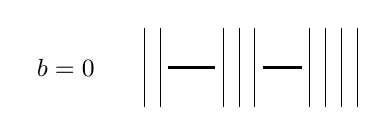
\begin{tikzpicture}
        
      \node at(0, .5)(a){\small{$b=0$}};
      \draw(1, 0) to (1, 1);
      \draw(1.2, 0) to (1.2, 1);
      \draw[line width = .3mm](1.3, .5) to (1.9, .5);
      \draw(2, 0) to (2, 1);
      \draw(2.2, 0) to(2.2, 1);
      \draw(2.4, 0) to (2.4, 1);
      \draw[line width = .3mm](2.5, .5) to (3, .5);
      \draw(3.1, 0) to (3.1, 1);
      \draw(3.3, 0) to (3.3, 1);
      \draw(3.5, 0) to (3.5, 1);
      \draw(3.7, 0) to (3.7, 1);
      \end{tikzpicture}}
  \end{minipage}
   \begin{minipage}{.45\textwidth}
   ~\centering
     ~\resizebox{.5\textwidth}{.1\textheight}{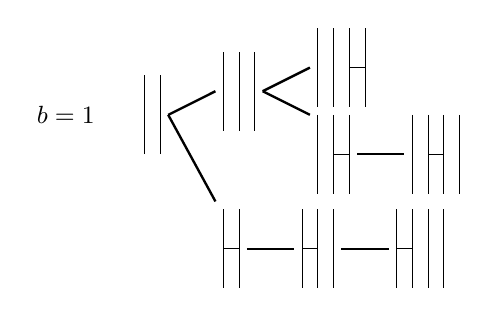
\begin{tikzpicture}
        
      \node at(0, .5)(a){\small{$b=1$}};
        \draw(1, 0) to (1, 1);
        \draw(1.2, 0) to (1.2, 1);
     \draw[line width = .3mm](1.3, .5) to (1.9, .8);
        \draw(2, .3) to (2, 1.3);
        \draw(2.2, .3) to(2.2, 1.3);
        \draw(2.4, .3) to (2.4, 1.3);
      \draw[line width = .3mm](2.5, .8) to (3.1, 1.1);
        \draw(3.2, 0.6) to (3.2, 1.6);
        \draw(3.4, 0.6) to (3.4, 1.6);
        \draw(3.6, 0.6) to (3.6, 1.6);
        \draw(3.6, 1.1) to (3.8, 1.1);
      \draw(3.8, 0.6) to (3.8, 1.6);

     \draw[line width = .3mm](2.5, .8) to (3.1, .5);
        \draw(3.2, .5) to (3.2, -.5);
        \draw(3.4, .5) to (3.4, -.5);
          \draw(3.4, 0) to (3.6, 0);                
        \draw(3.6, .5) to (3.6, -.5);


      \draw[line width = .3mm](3.7, 0) to (4.3, 0);
        \draw(4.4, .5) to (4.4, -.5);
        \draw(4.6, .5) to (4.6, -.5);
        \draw(4.8, .5) to (4.8, -.5);
                  \draw(4.6, 0) to (4.8, 0);                
        \draw(5, .5) to (5, -.5);


        \draw[line width= .3mm](1.3, .5) to (1.9, -.6);
          \draw(2, -.7) to (2, -1.7);
            \draw(2, -1.2) to (2.2, -1.2);
          \draw(2.2, -.7) to (2.2, -1.7);

        \draw[line width= .3mm](2.3, -1.2) to (2.9, -1.2);
        \draw(3, -.7) to (3, -1.7);
            \draw(3, -1.2) to (3.2, -1.2);
        \draw(3.2, -.7) to (3.2, -1.7);
        \draw(3.4, -.7) to (3.4, -1.7);
        \draw[line width= .3mm](3.5, -1.2) to (4.1, -1.2);
        \draw(4.2, -.7) to (4.2, -1.7);
            \draw(4.2, -1.2) to (4.4, -1.2);
        \draw(4.4, -.7) to (4.4, -1.7);
        \draw(4.6, -.7) to (4.6, -1.7);
        \draw(4.8, -.7) to (4.8, -1.7);
        




      \end{tikzpicture}}
      
    \end{minipage}
    \begin{minipage}{.45\textwidth}
     ~\centering
     ~\resizebox{.5\textwidth}{.2\textheight}{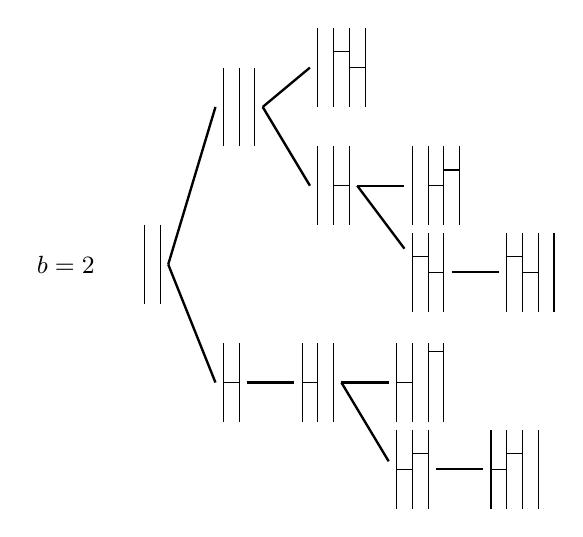
\begin{tikzpicture}
      \node at(0, 5.5){\small{$b=2$}};  
      %%t1
      \draw(1, 5) to (1, 6);
      \draw(1.2, 5) to (1.2, 6);
    \draw[line width = .3mm](1.3, 5.5) to (1.9, 7.5);
      \draw(2, 8) to (2, 7);
      \draw(2.2, 8) to (2.2, 7);
      \draw(2.4, 8) to (2.4, 7);
    \draw[line width = .3mm](2.5, 7.5) to (3.1, 8);
      \draw(3.2, 7.5) to (3.2, 8.5);
      \draw(3.4, 7.5) to (3.4, 8.5);
        \draw(3.4, 8.2) to (3.6, 8.2);
      \draw(3.6, 7.5) to (3.6, 8.5);
        \draw(3.6, 8) to (3.8, 8);
      \draw(3.8, 7.5) to (3.8, 8.5);

      %%tt2
    \draw[line width=.3mm](2.5, 7.5) to (3.1, 6.5);
      \draw(3.2, 7) to (3.2, 6);
      \draw(3.4, 7) to (3.4, 6);
        \draw(3.4, 6.5) to (3.6, 6.5);
      \draw(3.6, 7) to (3.6, 6);
    
    \draw[line width = .3mm](3.7, 6.5) to (4.3, 6.5);
      \draw(4.4, 6) to (4.4, 7);
      \draw(4.6, 6) to (4.6, 7);
        \draw(4.6, 6.5) to (4.8, 6.5);
      \draw(4.8, 6) to (4.8, 7);
        \draw(4.8, 6.7) to (5, 6.7);
      \draw(5, 6) to (5, 7);
    
    \draw[line width = .3mm](3.7, 6.5) to (4.3, 5.7);
      \draw(4.4, 5.9) to (4.4, 4.9);
        \draw(4.4, 5.6) to (4.6, 5.6);
      \draw(4.6, 5.9) to (4.6, 4.9);
        \draw(4.6, 5.4) to (4.8, 5.4);
      \draw(4.8, 5.9) to (4.8, 4.9);
    
   \draw[line width = .3mm](4.9, 5.4) to (5.5, 5.4);
      \draw(5.6, 5.9) to (5.6, 4.9);
        \draw(5.6, 5.6) to (5.8, 5.6);
      \draw(5.8, 5.9) to (5.8, 4.9);
        \draw(5.8, 5.4) to (6, 5.4);
      \draw(6, 5.9) to (6, 4.9);
      \draw(6.2, 5.9) to (6.2, 4.9);

    \draw[line width = .3mm](1.3, 5.5) to (1.9, 4);
    
        \draw(2, 4.5) to (2, 3.5);
          \draw(2, 4) to (2.2, 4);
        \draw(2.2, 4.5) to (2.2, 3.5);

    \draw[line width = .3mm](2.3, 4) to (2.9, 4);
        \draw(3, 4.5) to (3, 3.5);
          \draw(3, 4) to (3.2, 4);
        \draw(3.2, 4.5) to (3.2, 3.5);
        \draw(3.4, 4.5) to (3.4, 3.5);
    \draw[line width = .3mm](3.5, 4) to (4.1, 4);
    \draw[line width = .3mm](3.5, 4) to (4.1, 3);
      \draw(4.2, 4.5) to (4.2, 3.5);
        \draw(4.2, 4) to (4.4, 4);
      \draw(4.4, 4.5) to (4.4, 3.5);
      \draw(4.6, 4.5) to (4.6, 3.5);
        \draw(4.6, 4.4) to (4.8, 4.4);
      \draw(4.8, 4.5) to (4.8, 3.5);

      \draw(4.2, 3.4) to (4.2, 2.4);
        \draw(4.2, 2.9) to (4.4, 2.9);
      \draw(4.4, 3.4) to (4.4, 2.4);
        \draw(4.4, 3.1) to (4.6, 3.1);
      \draw(4.6, 3.4) to (4.6, 2.4);
    
    \draw[line width = .3mm](4.7, 2.9) to (5.3, 2.9);
        \draw(5.4, 3.4) to (5.4, 2.4);
          \draw(5.4, 2.9) to (5.6, 2.9);
        \draw(5.6, 3.4) to (5.6, 2.4);
          \draw(5.6, 3.1) to (5.8, 3.1);
        \draw(5.8, 3.4) to (5.8, 2.4);
        \draw(6.0, 3.4) to (6.0, 2.4);




    \end{tikzpicture}}
  \end{minipage}
  \begin{minipage}{.45\textwidth}
   ~\centering
   ~\resizebox{.5\textwidth}{.25\textheight}{\begin{tikzpicture}
      \node at(0, 5.5){\small{$b=3$}};
        %%t1
        \draw(1, 5) to (1, 6);
        \draw(1.2, 5) to (1.2, 6);
      \draw[line width = .3mm](1.3, 5.5) to (1.9, 7.5);
        \draw(2, 7) to (2, 8);
        \draw(2.2, 7) to (2.2, 8);
        \draw(2.4, 7) to (2.4, 8);
      \draw[line width = .3mm](2.5, 7.5) to (2.9, 9);
      \draw[line width = .3mm](2.5, 7.5) to (2.9, 6.5);
        %%Leaf1
        \draw(3, 9.5) to (3, 8.5);
          \draw(3, 9.4) to (3.2, 9.4);
        \draw(3.2, 9.5) to (3.2, 8.5);
          \draw(3.2, 9.2) to (3.4, 9.2);
        \draw(3.4, 9.5) to (3.4, 8.5);
          \draw(3.4, 9) to (3.6, 9);
        \draw(3.6, 9.5) to (3.6, 8.5);
        %%t2
        \draw(3, 7) to (3, 6);
        \draw(3.2, 7) to (3.2, 6);
          \draw(3.2, 6.5) to (3.4, 6.5);
        \draw(3.4, 7) to (3.4, 6);
        \draw[line width = .3mm](3.5, 6.5) to (4.1, 6.5);
        \draw[line width = .3mm](3.5, 6.5) to (4.1, 5.5);
        %%Leaf2
        \draw(4.2, 6) to (4.2, 7);
        \draw(4.4, 6) to (4.4, 7);
          \draw(4.4, 6.7) to (4.6, 6.7);
          \draw(4.4, 6.3) to (4.6, 6.3);
        \draw(4.6, 6) to (4.6, 7);
          \draw(4.6, 6.5) to (4.8, 6.5);
        \draw(4.8, 6) to (4.8, 7);

        \draw(4.2, 5.9) to (4.2, 4.9);
          \draw(4.2, 5.5) to (4.4, 5.5);
        \draw(4.4, 5.9) to (4.4, 4.9);
          \draw(4.4, 5.3) to (4.6, 5.3);
        \draw(4.6, 5.9) to (4.6, 4.9);
      \draw[line width = .3mm](4.7, 5.4) to (5.3, 5.4);
      %%leaf 3
        \draw(5.4, 4.9) to (5.4, 5.9);
          \draw(5.4, 5.5)to(5.6, 5.5);
        \draw(5.6, 4.9) to (5.6, 5.9);
          \draw(5.6, 5.3) to (5.8, 5.3);
        \draw(5.8, 4.9) to (5.8, 5.9);
          \draw(5.8, 5.5)to(6, 5.5);
        \draw(6.0, 4.9) to (6.0, 5.9);

      %%Line
      \draw[line width=.3mm](1.3, 5.5) to (1.9, 4);

        \draw(2, 4.5) to (2, 3.5);
          \draw(2, 3.6) to (2.2, 3.6);
        \draw(2.2, 4.5) to (2.2, 3.5);

      \draw[line width = .3mm](2.3, 4) to (2.9, 4);
        \draw(3.0, 4.5) to (3.0, 3.5);
          \draw(3, 3.6) to (3.2, 3.6);
        \draw(3.2, 4.5) to (3.2, 3.5);
      
        \draw(3.4, 4.5) to (3.4, 3.5);
      
        \draw[line width = .3mm](3.5, 4) to (4.1, 4.3);
      %%leaf 4
        \draw(4.2, 3.8) to (4.2, 4.8);
          \draw(4.2, 3.9) to (4.4, 3.9);
        \draw(4.4, 3.8) to (4.4, 4.8);
          \draw(4.4, 4.5) to (4.6, 4.5);
        \draw(4.6, 3.8) to (4.6, 4.8);
          \draw(4.6, 4.3) to (4.8, 4.3);
        \draw(4.8, 3.8) to (4.8, 4.8);

    \draw[line width = .3mm](3.5, 4) to (4.1, 3.5);
      \draw(4.2, 3.7) to (4.2, 2.7);
        \draw(4.2,  2.8) to (4.4, 2.8);
      \draw(4.4, 3.7) to (4.4, 2.7);
        \draw(4.4, 3) to (4.6, 3);
      \draw(4.6, 3.7) to (4.6, 2.7);

    \draw[line width = .3mm](4.7, 3.2) to (5.3, 3.9);
    %%leaf 5
      \draw(5.4, 4.4) to (5.4, 3.4);
        \draw(5.4, 3.5) to (5.6, 3.5);
        \draw(5.6, 3.7) to (5.8, 3.7);
        \draw(5.8, 3.9) to (6.0, 3.9);
      \draw(5.6, 4.4) to (5.6, 3.4);
      \draw(5.8, 4.4) to (5.8, 3.4);
      \draw(6.0, 4.4) to (6.0, 3.4);
   
    \draw[line width = .3mm](4.7, 3.2) to (5.3, 2.5);
    \draw(5.4, 3) to (5.4, 2);
      \draw(5.4, 2.1) to (5.6, 2.1);
      \draw(5.4, 2.5) to (5.6, 2.5);
    \draw(5.6, 3) to (5.6, 2);
      \draw(5.6, 2.3) to (5.8, 2.3);
    \draw(5.8, 3) to (5.8, 2);

    \draw[line width = .3mm](5.9, 2.5) to (6.4, 2.5);
    \draw(6.5, 3) to (6.5, 2);
      \draw(6.5, 2.1) to (6.7, 2.1);
      \draw(6.5, 2.5) to (6.7, 2.5);
    \draw(6.7, 3) to (6.7, 2);
      \draw(6.7, 2.3) to (6.9, 2.3);
    \draw(6.9, 3) to (6.9, 2);
    \draw(7.1, 3) to (7.1, 2);




    \end{tikzpicture}}
  \end{minipage}
   \begin{minipage}{.45\textwidth}
   ~\centering
   ~\resizebox{.5\textwidth}{.25\textheight}{\begin{tikzpicture}
      \node at(0, 5.5){\small{$b=4$}};
        %%t1
        \draw(1, 5) to (1, 6);
        \draw(1.2, 5) to (1.2, 6);
      \draw[line width = .3mm](1.3, 5.5) to (1.9, 7.5);
        \draw(2, 7) to (2, 8);
        \draw(2.2, 7) to (2.2, 8);
        \draw(2.4, 7) to (2.4, 8);
      \draw[line width = .3mm](2.5, 7.5) to (2.9, 9);
      \draw[line width = .3mm](2.5, 7.5) to (2.9, 7.5);
        %%Leaf1
        \draw(3, 9.5) to (3, 8.5);
          \draw(3, 9.4) to (3.2, 9.4);
        \draw(3.2, 9.5) to (3.2, 8.5);
          \draw(3.2, 9.2) to (3.4, 9.2);
        \draw(3.4, 9.5) to (3.4, 8.5);
          \draw(3.4, 9) to (3.6, 9);
        \draw(3.6, 9.5) to (3.6, 8.5);
        %%t2
        \draw(3, 7) to (3, 8);
        \draw(3.2, 7) to (3.2, 8);
          \draw(3.2, 7.5) to (3.4, 7.5);
        \draw(3.4, 7) to (3.4, 8);
        \draw[line width = .3mm](3.5, 7.5) to (4.1, 7.5);
        %%Leaf2
        \draw(4.2, 7) to (4.2, 8);
          \draw(4.2, 7.9) to (4.4, 7.9);
        \draw(4.4, 7) to (4.4, 8);
          \draw(4.4, 7.3) to (4.6, 7.3);
          \draw(4.4, 7.7) to (4.6, 7.7);
        \draw(4.6, 7) to (4.6, 8);
          \draw(4.6, 7.5) to (4.8, 7.5);s
        \draw(4.8, 7) to (4.8, 8);
        %%\draw[line width = .3mm](3.5, 6.5) to (4.1, 5.5);

        \draw[line width = .3mm](3.5, 7.5) to (4.1, 6.5);

        \draw(4.2, 6.9) to (4.2, 5.9);
          \draw(4.2, 6.4) to (4.4, 6.4);
        \draw(4.4, 6.9) to (4.4, 5.9);
          \draw(4.4, 6.2) to (4.6, 6.2);
        \draw(4.6, 6.9) to (4.6, 5.9);

        \draw[line width = .3mm](4.7, 6.4) to (5.3, 6.4);
      %%leaf 3
        \draw(5.4, 6.9) to (5.4, 5.9);
          \draw(5.4, 6.4) to (5.6, 6.4);
        \draw(5.6, 6.9) to (5.6, 5.9);
          \draw(5.6, 6.2) to (5.8, 6.2);
          \draw(5.6, 6.6) to (5.8, 6.6);
        \draw(5.8, 6.9) to (5.8, 5.9);
          \draw(5.8, 6.4) to (6.0, 6.4);
        \draw(6.0, 6.9) to (6.0, 5.9);


      \draw[line width = .3mm](1.3, 5.5) to (1.9, 3.5);
      \draw(1.9, 4) to (1.9, 3);
        \draw(1.9, 3.1) to (2.1, 3.1);
      \draw(2.1, 4) to (2.1, 3);

      \draw[line width = .3mm](2.2, 3.5) to (2.8, 4.1);
      
      \draw(2.9, 4.6) to (2.9, 3.6);
        \draw(2.9, 3.7) to (3.1, 3.7);
      \draw(3.1, 4.6) to (3.1, 3.6);
      \draw(3.3, 4.6) to (3.3, 3.6);

      \draw[line width = .3mm](3.4, 4.1) to (4,5.1);
      %%Leaf 4
      \draw(4.1, 5.6) to (4.1, 4.6);
        \draw(4.1, 4.7) to (4.3, 4.7);
        \draw(4.1, 5.5) to (4.3, 5.5);
      \draw(4.3, 4.6) to (4.3, 5.6);
        \draw(4.3, 5.3) to (4.5, 5.3);
      \draw(4.5, 4.6) to (4.5, 5.6);
        \draw(4.5, 5.1) to (4.7, 5.1);
      \draw(4.7, 4.6) to (4.7, 5.6);

      \draw[line width = .3mm](3.4, 4.1) to (4,3.1);
      \draw(4.1, 3.6) to (4.1, 2.6);
        \draw(4.1, 2.7) to (4.3, 2.7);
      \draw(4.3, 3.6) to (4.3, 2.6);
        \draw(4.3, 2.9) to (4.5, 2.9);
      \draw(4.5, 3.6) to (4.5, 2.6);

      \draw[line width = .3mm](4.6, 3.1) to (5.2, 3.8);
      %%leaf 5
      \draw(5.3, 4.3) to (5.3, 3.3);
        \draw(5.3, 3.4) to (5.5, 3.4);
      \draw(5.5, 4.3) to (5.5, 3.3);
        \draw(5.5, 3.6) to (5.7, 3.6);
      \draw(5.7, 4.3) to (5.7, 3.3);
        \draw(5.7, 3.8) to (5.9, 3.8);
        \draw(5.5, 4) to (5.7, 4);
      \draw(5.9, 4.3) to (5.9, 3.3);
      
      
      \draw[line width = .3mm](4.6, 3.1) to (5.2, 2.5);

      \draw(5.3, 3) to (5.3, 2);
        \draw(5.3, 2.1) to (5.5, 2.1);
        \draw(5.3, 2.5) to (5.5, 2.5);
      \draw(5.5, 3) to (5.5, 2);
        \draw(5.5, 2.3) to (5.7, 2.3);
      \draw(5.7, 3) to (5.7, 2);

      \draw[line width = .3mm](5.8, 2.5) to (6.4, 2.5);

      
      \draw(6.5, 3) to (6.5, 2);
        \draw(6.5, 2.1) to (6.7, 2.1);
        \draw(6.5, 2.5) to (6.7, 2.5);
      \draw(6.7, 3) to (6.7, 2);
        \draw(6.7, 2.3) to (6.9, 2.3);
      \draw(6.9, 3) to (6.9, 2);
        \draw(6.9, 2.5) to (7.1, 2.5);
      \draw(7.1, 2) to (7.1, 3);






    \end{tikzpicture}}
  \end{minipage}
  \begin{minipage}{.45\textwidth}
   ~\centering
   ~\resizebox{.5\textwidth}{.25\textheight}{\begin{tikzpicture}
      \node at(0, 5.5){\small{$b=5$}};
        %%t1
        \draw(1, 5) to (1, 6);
        \draw(1.2, 5) to (1.2, 6);
      \draw[line width = .3mm](1.3, 5.5) to (1.9, 7.5);
        \draw(2, 7) to (2, 8);
        \draw(2.2, 7) to (2.2, 8);
        \draw(2.4, 7) to (2.4, 8);
      \draw[line width = .3mm](2.5, 7.5) to (2.9, 9);
      \draw[line width = .3mm](2.5, 7.5) to (2.9, 7.5);
        %%Leaf1
        \draw(3, 9.5) to (3, 8.5);
          \draw(3, 9.4) to (3.2, 9.4);
        \draw(3.2, 9.5) to (3.2, 8.5);
          \draw(3.2, 9.2) to (3.4, 9.2);
        \draw(3.4, 9.5) to (3.4, 8.5);
          \draw(3.4, 9) to (3.6, 9);
        \draw(3.6, 9.5) to (3.6, 8.5);
        %%t2
        \draw(3, 7) to (3, 8);
        \draw(3.2, 7) to (3.2, 8);
          \draw(3.2, 7.5) to (3.4, 7.5);
        \draw(3.4, 7) to (3.4, 8);
        \draw[line width = .3mm](3.5, 7.5) to (4.1, 7.5);
        %%Leaf2
        \draw(4.2, 7) to (4.2, 8);
          \draw(4.2, 7.9) to (4.4, 7.9);
        \draw(4.4, 7) to (4.4, 8);
          \draw(4.4, 7.3) to (4.6, 7.3);
          \draw(4.4, 7.7) to (4.6, 7.7);
        \draw(4.6, 7) to (4.6, 8);
          \draw(4.6, 7.5) to (4.8, 7.5);
        \draw(4.8, 7) to (4.8, 8);
        \draw[line width = .3mm](3.5, 7.5) to (4.1, 6.5);

        \draw[line width = .3mm](3.5, 7.5) to (4.1, 6.5);

        \draw(4.2, 6.9) to (4.2, 5.9);
          \draw(4.2, 6.4) to (4.4, 6.4);
        \draw(4.4, 6.9) to (4.4, 5.9);
          \draw(4.4, 6.2) to (4.6, 6.2);
        \draw(4.6, 6.9) to (4.6, 5.9);

        \draw[line width = .3mm](4.7, 6.4) to (5.3, 6.4);
      %%leaf 3
        \draw(5.4, 6.9) to (5.4, 5.9);
          \draw(5.4, 6.4) to (5.6, 6.4);
          \draw(5.4, 6.8) to (5.6, 6.8);
        \draw(5.6, 6.9) to (5.6, 5.9);
          \draw(5.6, 6.2) to (5.8, 6.2);
          \draw(5.6, 6.6) to (5.8, 6.6);
        \draw(5.8, 6.9) to (5.8, 5.9);
          \draw(5.8, 6.4) to (6.0, 6.4);
        \draw(6.0, 6.9) to (6.0, 5.9);


      \draw[line width = .3mm](1.3, 5.5) to (1.9, 3.5);
      \draw(1.9, 4) to (1.9, 3);
        \draw(1.9, 3.1) to (2.1, 3.1);
      \draw(2.1, 4) to (2.1, 3);

      \draw[line width = .3mm](2.2, 3.5) to (2.8, 4.1);
      
      \draw(2.9, 4.6) to (2.9, 3.6);
        \draw(2.9, 3.7) to (3.1, 3.7);
      \draw(3.1, 4.6) to (3.1, 3.6);
      \draw(3.3, 4.6) to (3.3, 3.6);

      \draw[line width = .3mm](3.4, 4.1) to (4,5.1);
      %%Leaf 4
      \draw(4.1, 5.6) to (4.1, 4.6);
        \draw(4.1, 4.7) to (4.3, 4.7);
        \draw(4.1, 5.5) to (4.3, 5.5);
      \draw(4.3, 4.6) to (4.3, 5.6);
        \draw(4.3, 5.3) to (4.5, 5.3);
      \draw(4.5, 4.6) to (4.5, 5.6);
        \draw(4.5, 5.1) to (4.7, 5.1);
      \draw(4.7, 4.6) to (4.7, 5.6);

      \draw[line width = .3mm](3.4, 4.1) to (4,3.1);
      \draw(4.1, 3.6) to (4.1, 2.6);
        \draw(4.1, 2.7) to (4.3, 2.7);
      \draw(4.3, 3.6) to (4.3, 2.6);
        \draw(4.3, 2.9) to (4.5, 2.9);
      \draw(4.5, 3.6) to (4.5, 2.6);

      \draw[line width = .3mm](4.6, 3.1) to (5.2, 3.8);
      %%leaf 5
      \draw(5.3, 4.3) to (5.3, 3.3);
        \draw(5.3, 3.4) to (5.5, 3.4);
        \draw(5.3, 4.2) to (5.5, 4.2);

      \draw(5.5, 4.3) to (5.5, 3.3);
        \draw(5.5, 3.6) to (5.7, 3.6);
      \draw(5.7, 4.3) to (5.7, 3.3);
        \draw(5.7, 3.8) to (5.9, 3.8);
        \draw(5.5, 4) to (5.7, 4);
      \draw(5.9, 4.3) to (5.9, 3.3);
      
      
      \draw[line width = .3mm](4.6, 3.1) to (5.2, 2.5);

      \draw(5.3, 3) to (5.3, 2);
        \draw(5.3, 2.1) to (5.5, 2.1);
        \draw(5.3, 2.5) to (5.5, 2.5);
      \draw(5.5, 3) to (5.5, 2);
        \draw(5.5, 2.3) to (5.7, 2.3);
      \draw(5.7, 3) to (5.7, 2);

      \draw[line width = .3mm](5.8, 2.5) to (6.4, 2.5);

      
      \draw(6.5, 3) to (6.5, 2);
        \draw(6.5, 2.1) to (6.7, 2.1);
        \draw(6.5, 2.5) to (6.7, 2.5);
      \draw(6.7, 3) to (6.7, 2);
        \draw(6.7, 2.3) to (6.9, 2.3);
        \draw(6.7, 2.7) to (6.9, 2.7);
      \draw(6.9, 3) to (6.9, 2);
        \draw(6.9, 2.5) to (7.1, 2.5);
      \draw(7.1, 2) to (7.1, 3);






    \end{tikzpicture}}
  \end{minipage}
   \begin{minipage}{.45\textwidth}
   ~\centering
   ~\resizebox{.5\textwidth}{.25\textheight}{\begin{tikzpicture}
      \node at(0, 5.5){\small{$b=6$}};
        %%t1
        \draw(1, 5) to (1, 6);
        \draw(1.2, 5) to (1.2, 6);
      \draw[line width = .3mm](1.3, 5.5) to (1.9, 7.5);
        \draw(2, 7) to (2, 8);
        \draw(2.2, 7) to (2.2, 8);
        \draw(2.4, 7) to (2.4, 8);
      \draw[line width = .3mm](2.5, 7.5) to (2.9, 9);
      \draw[line width = .3mm](2.5, 7.5) to (2.9, 7.5);
        %%Leaf1
        \draw(3, 9.5) to (3, 8.5);
          \draw(3, 9.4) to (3.2, 9.4);
        \draw(3.2, 9.5) to (3.2, 8.5);
          \draw(3.2, 9.2) to (3.4, 9.2);
        \draw(3.4, 9.5) to (3.4, 8.5);
          \draw(3.4, 9) to (3.6, 9);
        \draw(3.6, 9.5) to (3.6, 8.5);
        %%t2
        \draw(3, 7) to (3, 8);
        \draw(3.2, 7) to (3.2, 8);
          \draw(3.2, 7.5) to (3.4, 7.5);
        \draw(3.4, 7) to (3.4, 8);
        \draw[line width = .3mm](3.5, 7.5) to (4.1, 7.5);
        %%Leaf2
        \draw(4.2, 7) to (4.2, 8);
          \draw(4.2, 7.9) to (4.4, 7.9);
        \draw(4.4, 7) to (4.4, 8);
          \draw(4.4, 7.3) to (4.6, 7.3);
          \draw(4.4, 7.7) to (4.6, 7.7);
        \draw(4.6, 7) to (4.6, 8);
          \draw(4.6, 7.5) to (4.8, 7.5);
        \draw(4.8, 7) to (4.8, 8);
        \draw[line width = .3mm](3.5, 7.5) to (4.1, 6.5);

        \draw[line width = .3mm](3.5, 7.5) to (4.1, 6.5);

        \draw(4.2, 6.9) to (4.2, 5.9);
          \draw(4.2, 6.4) to (4.4, 6.4);
        \draw(4.4, 6.9) to (4.4, 5.9);
          \draw(4.4, 6.2) to (4.6, 6.2);
        \draw(4.6, 6.9) to (4.6, 5.9);

        \draw[line width = .3mm](4.7, 6.4) to (5.3, 6.4);
      %%leaf 3
        \draw(5.4, 6.9) to (5.4, 5.9);
          \draw(5.4, 6.4) to (5.6, 6.4);
          \draw(5.4, 6.8) to (5.6, 6.8);
        \draw(5.6, 6.9) to (5.6, 5.9);
          \draw(5.6, 6.2) to (5.8, 6.2);
          \draw(5.6, 6.6) to (5.8, 6.6);
        \draw(5.8, 6.9) to (5.8, 5.9);
          \draw(5.8, 6.4) to (6.0, 6.4);
        \draw(6.0, 6.9) to (6.0, 5.9);


      \draw[line width = .3mm](1.3, 5.5) to (1.9, 3.5);
      \draw(1.9, 4) to (1.9, 3);
        \draw(1.9, 3.1) to (2.1, 3.1);
      \draw(2.1, 4) to (2.1, 3);

      \draw[line width = .3mm](2.2, 3.5) to (2.8, 4.1);
      
      \draw(2.9, 4.6) to (2.9, 3.6);
        \draw(2.9, 3.7) to (3.1, 3.7);
      \draw(3.1, 4.6) to (3.1, 3.6);
      \draw(3.3, 4.6) to (3.3, 3.6);

      \draw[line width = .3mm](3.4, 4.1) to (4,5.1);
      %%Leaf 4
      \draw(4.1, 5.6) to (4.1, 4.6);
        \draw(4.1, 4.7) to (4.3, 4.7);
        \draw(4.1, 5.5) to (4.3, 5.5);
      \draw(4.3, 4.6) to (4.3, 5.6);
        \draw(4.3, 5.3) to (4.5, 5.3);
      \draw(4.5, 4.6) to (4.5, 5.6);
        \draw(4.5, 5.1) to (4.7, 5.1);
      \draw(4.7, 4.6) to (4.7, 5.6);

      \draw[line width = .3mm](3.4, 4.1) to (4,3.1);
      \draw(4.1, 3.6) to (4.1, 2.6);
        \draw(4.1, 2.7) to (4.3, 2.7);
      \draw(4.3, 3.6) to (4.3, 2.6);
        \draw(4.3, 2.9) to (4.5, 2.9);
      \draw(4.5, 3.6) to (4.5, 2.6);

      \draw[line width = .3mm](4.6, 3.1) to (5.2, 3.8);
      %%leaf 5
      \draw(5.3, 4.3) to (5.3, 3.3);
        \draw(5.3, 3.4) to (5.5, 3.4);
        \draw(5.3, 4.2) to (5.5, 4.2);

      \draw(5.5, 4.3) to (5.5, 3.3);
        \draw(5.5, 3.6) to (5.7, 3.6);
      \draw(5.7, 4.3) to (5.7, 3.3);
        \draw(5.7, 3.8) to (5.9, 3.8);
        \draw(5.5, 4) to (5.7, 4);
      \draw(5.9, 4.3) to (5.9, 3.3);
      
      
      \draw[line width = .3mm](4.6, 3.1) to (5.2, 2.5);

      \draw(5.3, 3) to (5.3, 2);
        \draw(5.3, 2.1) to (5.5, 2.1);
        \draw(5.3, 2.5) to (5.5, 2.5);
      \draw(5.5, 3) to (5.5, 2);
        \draw(5.5, 2.3) to (5.7, 2.3);
      \draw(5.7, 3) to (5.7, 2);

      \draw[line width = .3mm](5.8, 2.5) to (6.4, 2.5);

      
      \draw(6.5, 3) to (6.5, 2);
        \draw(6.5, 2.1) to (6.7, 2.1);
        \draw(6.5, 2.5) to (6.7, 2.5);
      \draw(6.7, 3) to (6.7, 2);
        \draw(6.7, 2.3) to (6.9, 2.3);
        \draw(6.7, 2.7) to (6.9, 2.7);
      \draw(6.9, 3) to (6.9, 2);
        \draw(6.9, 2.5) to (7.1, 2.5);
        \draw(6.9, 2.9) to (7.1, 2.9);
      \draw(7.1, 2) to (7.1, 3);






    \end{tikzpicture}}
  \end{minipage}
  
  

     
  \caption{The forest for all ladders in $L_{4}$ generated by the Cyclic Bar Algorithm. The leaf nodes present a possibly correct candidate ladder. 
  If the ladder in the leaf has enough bars, then it is a legitimate ladder in the tree.}
  \label{Fig:CanLForest}
\end{figure}
\end{center}
It has been stated that the forest produced by the Cyclic Bar algorithm generates
$L_{n}$. This claim will be proven below.


\begin{theorem}
  The forest produced by {\sc CyclicBar} generates $L_{n}$
\end{theorem}


\begin{proof}
  The proof is done by way of a combinatorial proof and induction. Rather than list ladders, we shall list permutations using the same method.  
  Let $List(n, k)$ be the listing of permutations of order $n$ with $k$ inversions. The hypothesis is that $List(n, k)=\sum_{m=0}^{k} List(n-1, m)$ 
  given $n>1$ and $k \geq 0$.
  The base case is $n=2$ and $k=0$. We know that the identity permutation of order $1$ has no inversions. We know that the list containing the identity 
  permutation of order $1$ is of length one. We know that the list containing the identity permutation of order $2$ is of length one. By appending the 
  value $2$ to the only permutation in the list $List(1, 0)$ we get the only permutation in the list $List(2, 0)$. Therefore the base case checks out.
  
  Suppose we have the list of permutations for $List(n-1, 0) \dots List(n-1, k)$. We want to show that we can insert the $nth$ element into each of the
  permutations in each of these lists such that the resulting permutations have $n$ elements with $k$ inversions. Partition $k$ into $k'$ and $k''$. Note that 
  $k'+k''=k$.
  Let $k'$ equal the number of inversions formed by the $nth$ element. Let $k''$ equal the number of elements not formed by the $nth$ element.
  We can look at the $List(n-1, 0) \dots List(n-1, k)$ as lists of permutations with $k''$ inversions. So we write 
  $List(n-1, 0) \dots List(n-1, k)$ as $List(n-1, k''=0) \dots List(n-1, k''=k)$. When $k''=0$ we know $List(n-1, 0)$ has one permutation, thus $k'=k$.
  The $nth$ element must be positioned $k'$ positions to the left of the $nth$ position in this one permutation from $List(n-1, 0)$ to form a permutation of order $n$ with $k$ inversions. 
  In general, we can say that for each of the permutations from each of the $List(n-1, k'')$, we know that the $nth$ element must be positioned $k-k''$ to the left of the $nth$ position in order to 
  ce a permutation of length $n$ with $k$ inversions. Thus, by exhaustively inserting the $nth$ element in all $k-k''=k'$ positions to the left of the $nth$ position 
  in all permutations from all $List(n-1, k'')$, we get all permutations of order $n$ with $k$ inversions. 
  Therefore $List(n, k) = List(n, k') + \sum_{k''=0}^{k} List(n-1, k'') $.
  Seeing as an inversion in a permutation corresponds to a bar in 
  a ladder, then by using this same proof on ladders, we can generate all ladders with $k$ bars. 
  Which is to say that $ladders(n, k) = Ladders(n, k') + \sum_{k''=0}^{k} Ladders(n-1, k'')$.
  In order to list $L_{n}$ simply apply this same logic for all $k$ bars for $0 \leq k \leq n(n-1)/2$. To see an example of the above proof for $List(4, 2)$ refer to Table~\ref{Table:List4,2}.

\end{proof}

\begin{table}
  \begin{tabular}{|p{2cm}||p{2cm}||p{2cm}||p{2cm} ||p{2cm} ||p{2cm}||}
     \hline
        \small{$n$ value}& \small{$k$ value} & \small{$k''$ value} & \small{$k'$ value} &\small{$L($n-1$, k'')$} & \small{$L(n, k)$}\\
        \hline
        \small{$4$} & \small{$2$} & \small{$0$} & \small{$2$} & \small{$(1,2,3)$} & \small{$(1,4,2,3)$} \\
        \hline
        \small{$4$} & \small{$2$} & \small{$1$} & \small{$1$} & \small{$(1,3,2)$} & \small{$(1,3,4,2)$} \\
        \small{$4$} & \small{$2$} & \small{$1$} & \small{$1$} & \small{$(2,1,3)$} & \small{$(2,1,4,3)$} \\
        \hline
        \small{$4$} & \small{$2$} & \small{$2$} & \small{$0$} & \small{$(3,1,2)$} & \small{$(3,1,2,4)$} \\                
        \small{$4$} & \small{$2$} & \small{$2$} & \small{$0$} & \small{$(2,3,1)$} & \small{$(2,3,1,4)$} \\
        \hline
  \end{tabular}
  \caption{The table showing all $List(4, 2)$ derived from $List(3, 0) \dots List(3, 2) + List(4, k')$}
  \label{Table:List4,2}
\end{table}



\section{Results}
    In the results section, the runtimes of the two algorithms will be provided. The run times are done without printing the ladders. 
    When the ladders are printed, the runtime increases by a substantial amount. 
    The runtime for each algorithm for $n=12$ will be provided in table~\ref{Table:ListingResults}. 
    In the analysis section, the table will be further analyzed along with 
    the time and space complexity for each algorithm.
 \begin{center}
    \begin{table}
        \centering
    \begin{tabular}{ |p{3cm}||p{3cm}|p{3cm}|}
        \hline
        \multicolumn{3}{|c|}{Runtimes for generating $CanL\{\pi_{n}\}$ in seconds} \\
        \hline
            $n$ value& Cyclic Bar & Modified SJT\\
        \hline
            1   & 0.000000    &0.000000\\
            \hline
            2 &   0.000000  & 0.000000\\

            \hline
            3 &0.000000 & 0.000000\\
            \hline
            4 &0.000000 & 0.000000\\
            \hline
            5 &   0.000000  & 0.000000\\
            \hline
            6 & 0.000000  & 0.000000  \\
            \hline
            7 & 0.000000  & 0.000000\\
            \hline
            8 & 0.000000 & 0.000000\\
            \hline
            9 & 0.093750 & 0.000000\\
            \hline
            10 & 0.968750 & 0.031250\\
            \hline

            11 & 12.718750 & 0.250000\\
            \hline 
            12 & 174.312500 & 2.781250\\
        \hline
    \end{tabular}
    \caption{The table with the runtimes for listing $CanL\{\pi_{n}\}$ using the Cyclic Bar Algorithm and Modified SJT Algorithm.}
    \label{Table:ListingResults}
    \end{table}
\end{center}\pagebreak

\section{Analysis}
From looking at the table in the results section, it is clear that the {\sc modifiedSJT} algorithm performs 
better than the  |{\sc CyclicBar} algorithm. The reason(s) for this disparity in performance 
will be analyzed. Following this analysis, areas of application and practical relevance for the Listing Problem 
will be discussed along with concluding remarks.

\subsection{Performance Analysis}
    As $n \geq 9$ there is a noticeable difference between the runtimes of the two algorithms by a sizable order 
    of magnitude. Clearly the {\sc ModifiedSJT} algorithm performs better than the {\sc CyclicBar} algorithm. The reason(s) 
    for this improved performance are the difference in time complexities between the two algorithms.
    The time complexity for the {\sc ModifiedSJT} algorithm is constant amortized time per ladder. The time will be proven in the following lemma.
    \begin{lemma}
        The amortized time for {\sc ModifiedSJT} is $O(1)$ per ladder.
    \end{lemma}
    \begin{proof}
        Each iteration of the for loop inserts or removes a bar, thus creating a new ladder. This is done in constant time 
        per addition or removal of a bar. 
    \end{proof}
    \begin{lemma}
       The amortized time for the  {\sc CyclicBar} algorithm is $O(n^{2}) + n^{2})$ per ladder.
    \end{lemma}
    \begin{proof}
        The first $n^{2}$ term is a result of the for loop that is executed for $k=2,3, \dots n$. This for loop runs 
        from $1$ to $k$ for each value of $k$. Thus, the for loop is executed $1 + 2 + 3 + 4, ... + n-1$ times. This summation 
        is equal to $((n-1)n-2)/2$ which is reduced to $n^{2}$. There is also the second $n^{2}$ term pertaining to backtracking. 
        Once $currenLimit \geq n$, then the algorithm 
        begins to back-track. Each time $currentLimit$ increases from $n$ to $n(n-1)/2$ the number of back-tracks increases by one per 
        $currentLimit$ level.
       Thus, there are $1 + 2 + 3 + 4, ... +  ((n(n-1))/2 - n)) + 1$ back-tracks required, which is reduced to $n^{2}$. Thus, the amortized  
       time per ladder is $O(n^{2}) + n^{2})$.
    \end{proof}

    The space complexity is the same for the two algorithms. Both require a two dimensional ladder data structure whose dimensions 
    are $(2(n-1)-1)(n-1)$. Therefore the space complexity for the algorithms is $O(n^{2})$.

    \subsection{Applications}
    The applications for generating $CanL\{\pi_{n}\}$ are currently unknown to me insofar as this problem has yet to be solved to my knowledge. 
    However, if I am to be granted some speculation, I could provide some hypothetical scenarios in which listing $CanL\{\pi_{n}\}$ could 
    be of interest. The first hypothetical application would be to model an \emph{oblivious sorting system} for $n!$ permutations. An oblivious 
    sorting system is a system such that the sorting operations are done irrespective of the data being passed to the system~\cite{A7}. Recall 
    that a bar in a ladder simply swaps two adjacent elements in a permutation. Due to the static nature of each ladder, the swap operation 
    resulting from two elements in a permutation crossing a bar is unchanging. 
    Seeing as each ladder in $CanL\{\pi_{n}\}$ sorts the corresponding permutation of order $n$, one can implement all of $CanL\{\pi_{n}\}$ 
    for some arbitrary $n$ value and then pass each permutation of order $n$ through its respective ladder from $CanL\{pi_{n}\}$ 
    resulting in each permutation being sorted. The ladders from $CanL\{\pi_{n}\}$ only need to be generated once and saved to disk 
    or implemented in hardware. 

\chapter{The Minimum Height Problem}
\label{chapter:minheightproblem}

In this chapter we describe a canonical ladder for each $OptL\{\pi}\}$. We then provide a number of equations to calculate the 
location of the bar in the canonical ladder; depending on the configuration of $\pi$, we use different 
equations for calculating the location of the bar. We then define the data structure used to represent the canonical ladder. 
Using the data structure, we provide an algorithm for creating the canonical ladder for any $\pi$ of order $n$. Lastly, 
we describe the listing problem in relation to the canonical ladder. To see the canonical ladder for $(3,5,4,1,2)$, 
refer to Figure~\ref{Fig:Route}.
\begin{figure}[h]
	\centering
	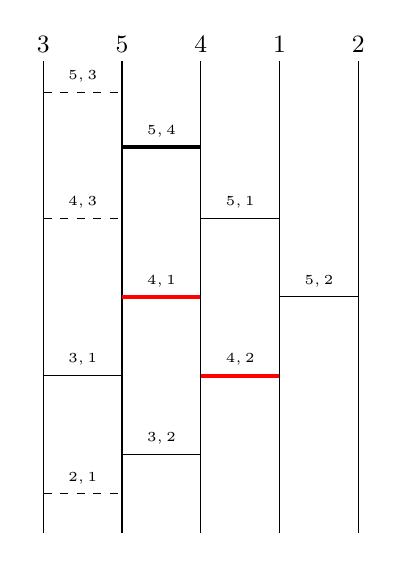
\begin{tikzpicture}
		\draw(0, 0) to (0, 6);
            \node at(.5, 5.8){\tiny{$5,3$}};
			\draw[dashed](0, 5.6) -- (1, 5.6);

            \node at(0.5, 4.2){\tiny{$4,3$}};
            \draw[dashed](0, 4) -- (1, 4);
			\node at(.5, 2.2){\tiny{$3,1$}};
			\draw(0, 2) to (1, 2);

            \draw[dashed](0, 0.5) -- (1, .5);
            \node at(.5, .7){\tiny{$2,1$}};
		\draw(1, 0) to (1, 6);
			\node at(1.5, 5.1){\tiny{$5,4$}};
			\draw[line width=.5mm](1, 4.9) to (2, 4.9);

			\node at(1.5, 3.2){\tiny{$4,1$}};
			\draw[line width=.5mm, red](1, 3.0) to (2, 3.0);

			\node at(1.5, 1.2){\tiny{$3,2$}};
			\draw(1, 1) to (2, 1);
	%		\node at(.75, .9){\tiny{$3,2$}};
	%		\draw(.5, .7) to (1, .7);
		\draw(2, 0) to (2, 6);

			\node at(2.5, 4.2){\tiny{$5,1$}};
			\draw(2, 4) to (3, 4);


			\node at(2.5, 2.2){\tiny{$4,2$}};
			\draw[line width=.5mm, red](2, 2) to (3, 2);
			%\node at(1.25, 2.1){\tiny{$4,1$}};
			%\draw[line width=.5mm, red ](1, 1.9) to (1.5, 1.9);
			%\node at(1.25, 1.3){\tiny{$5,2$}};
			%\draw(1, 1.1) to(1.5, 1.1);
		\draw(3, 0) to (3, 6);
			
			\node at(3.5, 3.2){\tiny{$5,2$}};
			\draw(3, 3.0) to (4, 3.0);	
		%\node at(1.75, 1.7){\tiny{$4,2$}};
			%\draw[line width=.5mm, red ](1.5, 1.5) to (2, 1.5);
			%\node at(1.75, .9){\tiny{$5,4$}};
			%\draw[line width=.5mm, red ](1.5, .7) to (2, .7);
		\draw(4, 0) to (4, 6);


		\node at(0.0, 6.2){\small{$3$}};
		\node at(1, 6.2){\small{$5$}};
		\node at(2.0, 6.2){\small{$4$}};
		\node at(3, 6.2){\small{$1$}};
		\node at(4, 6.2){\small{$2$}};
	\end{tikzpicture}
	\caption{The canonical ladder for $(3,5,4,1,2)$. Bars $(5,4),(4,1),(4,2)$ are part of the route of 
    $4$, but only the red bars are associated with the route of $4$.}
	\label{Fig:Route}
\end{figure}


\section{The Canonical Ladder in Detail}
In this section, we fully define the canonical ladder corresponding to $\pi$. We first define the associated terminology in order 
to provide a comprehensive definition of the canonical ladder.
Let the \emph{route} of an element be the sequence of bars the element travels along in order to reach its final position in the 
sorted permutation. The bars are read from top to bottom. In Figure~\ref{Fig:Route}, the bars $(5,4),(4,1)$ and $(4,2)$ compose the route of $4$. 
For every bar, two elements cross the bar, therefore \emph{bar association} is the association of a bar with the greater of the two elements that 
cross it. For example, in Figure~\ref{Fig:Route}, element $4$ has the bars $(5,4),(4,1)$ and 
$(4,2)$ in its route, however only bars $(4,1)$ and $(4,2)$ are associated with element $4$. Let the \emph{absence of a bar} corresponding to 
two uninverted elements in $\pi$, $x>y$, be defined as a dashed, horizontal line spanning across a column in the ladder. 
We say \emph{absence of a bar association} is the association of the absence of a bar with the greater of the two elements that form it. 
For example,$(5,3)$ are uninverted in $(3,5,4,1,2)$, therefore the absence of the bar is associated with $5$. 
For each element $2 \leq x \leq n \in \pi$, we define the \emph{associated diagonal of x} as a diagonal with $x-1$ 
row and column coordinates, having one endpoint at $(2n-2x+1, 1)$ and the other endpoint at $(2n-x-1,x-1)$.  
At each row and column in the associated diagonal of $x$, either a bar associated with $x$ or the absence of a bar associated with $x$ exists. 
For an example of the associated diagonals for the ladder corresponding to $(3,4,2,1,5)$ refer to Figure~\ref{fig:my_label}. 
\begin{figure}[h]
    \centering
    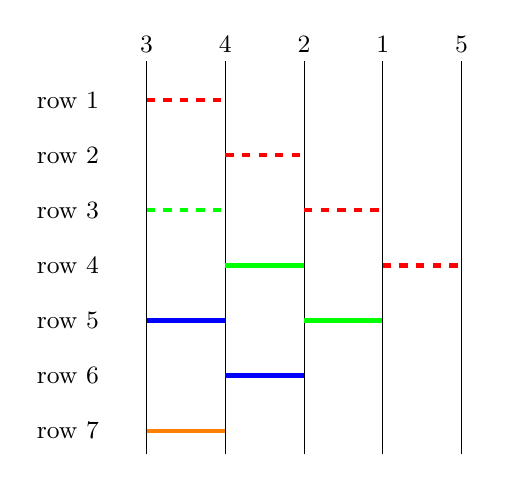
\begin{tikzpicture}
        \draw(0,0) to (0,5);
            \draw[red, dashed, line width=0.55mm](0, 4.5) -- (1,4.5);
            \draw[green, dashed, line width=0.55mm](0, 3.1) -- (1,3.1);
            \draw[blue, line width=0.55mm](0, 1.7) to (1,1.7);
            \draw[orange, line width=0.55mm](0, 0.3) to (1,0.3);

        \draw(1,0) to (1,5);
            \draw[red, dashed, line width=0.55mm](1, 3.8) -- (2,3.8);
            \draw[green, line width=0.55mm](1, 2.4) to (2,2.4);
            \draw[blue, line width=0.55mm](1, 1.0) to (2,1.0);
        \draw(2,0) to (2,5);
           \draw[red, dashed, line width=0.55mm](2, 3.1) -- (3,3.1);
            \draw[green, line width=0.55mm](2, 1.7) to (3,1.7);
        \draw(3,0) to (3,5);
         \draw[red, dashed, line width=0.55mm](3, 2.4) -- (4,2.4);
        \draw(4,0) to (4,5);

        \node at (-1, 4.5){\small{row 1}};
        \node at (-1, 3.8){\small{row 2}};
        \node at (-1, 3.1){\small{row 3}};
        \node at (-1, 2.4){\small{row 4}};
        \node at (-1, 1.7){\small{row 5}};
        \node at (-1, 1.0){\small{row 6}};
        \node at (-1, 0.3){\small{row 7}};

        \node at(0, 5.2){\small{$3$}};
        \node at(1, 5.2){\small{$4$}};
        \node at(2, 5.2){\small{$2$}};
        \node at(3, 5.2){\small{$1$}};
        \node at(4, 5.2){\small{$5$}};

    \end{tikzpicture}
    \caption{The associated diagonal of $5$ is in red, the associated diagonal of $4$ is in green, the associated diagonal of $3$ is in blue, and the associated diagonal of $2$ is in orange.}
    \label{fig:my_label}
\end{figure}

With the definition of the associated diagonal, we are now able to fully define the \emph{canonical ladder} as 
the ladder such that for each element $2 \leq x \leq n$, each bar, and absence of a bar, associated with $x$ exists 
along the associated diagonal of $x$. %Given $\pi$, we construct $CL(\pi)$ by using equation~\ref{getCordEqn} found in section 
%\textbf{Calculating the Location of a Bar for an Arbitrary $CL(\pi_{n})$}, 
%and Algorithm~\ref{Alg:RootLadder} found in section \textbf{Algorithm: Create Canonical}. 
We note that the two aforementioned figures, Figure~\ref{Fig:Route} and Figure~\ref{fig:my_label}, are the canonical ladders 
corresponding to each of their respective permutations. We use $CL(\pi)$ as shorthand notation for `the canonical ladder corresponding 
to a permutation of order $n$'. 

\section{Locating the Bar for a Given Inversion in an Arbitrary $CL(\pi)$}
In this section, we provide an equation for locating the bar in the canonical ladder associated with a given inversion, 
in an arbitrary permutation 
of order $n$. As previously stated, every bar associated with some element $x$ exists along the associated diagonal of $x$ 
within the canonical ladder. 
We use Equation~\ref{getCordEqn}, to determine the row and column for the bar corresponding 
to two elements, $x>y$, along the associated diagonal of $x$. 
Let $\pi$ be an arbitrary permutation of order $n$. Let 
$pos(x)$ be the index of $x \in \pi$. To calculate the row and column of the bar, or absence of a bar, for a pair of elements 
$x>y$, we first map $x$ to a new index termed $pos'(x)$. Let $pos'(x)$ equal $pos(x)$ minus the number of elements greater than $x$ and 
 to the left of $x$ in $\pi$. 
For example, given $\pi=(3,2,7,4,8,5,6,9,1)$, 
suppose $x=6$, then $pos'(6)=pos(6)-2=5$. 
Once we have calculated $pos'(x)$ we use a similar method to calculate $pos'(y)$. $pos'(y)$ equals 
$pos(y)$ minus the number of elements greater than $y$ and to the left of $y$ excluding $x$. For example, suppose $x$ is $7$ and 
$y$ is $5$, then $pos'(y)$ is $pos(y)-1=5$. Once we have $pos'(x)$ and $pos'(y)$, we use Equation~\ref{getCordEqn} 
to return the row and column for the bar, or absence of the bar,  
along the associated diagonal of $x$.
\begin{equation}\label{getCordEqn}
\resizebox{.9\textwidth}{!}{
\[   
    (row,column)=
    \begin{cases}
        ((2n - x - 1) - (x - pos'(y))+1,(x-1)-(x-pos'(y))+1) & \text{if $pos'(x)>pos'(y)$} \\ 
        ((2n - x - 1) - (x-pos'(y)), (x-1) - (x-pos'(y)) & \text{if $pos'(y)>pos'(x)$}
    \end{cases}
\]
}
\end{equation}

Given the inversion $(7,5) \in (3,2,7,4,8,5,6,9,1)$, we calculate the row and column of the bar $(7,5)$ using the second case. We 
get $row=(18 - 7 - 1) - (7 - 5)=8$ and $col=6-(7-5)=4$. To calculate $pos'(x)$ and $pos'(y)$, is linear amortized time. Once $pos'(x)$ 
and $pos'(y)$ are calculated,  returns the location in $O(1)$ time. 
We can use Equation~\ref{getCordEqn} to look up the location of any bar for a given $\pi$. 
In Figure~\ref{Fig:CanLArbitrary} we see $CL(3,2,7,4,8,5,6,9,1)$, where each row and column is calculated using Equation~\ref{getCordEqn}. 
\pagebreak
\begin{figure}[t]
    \centering
    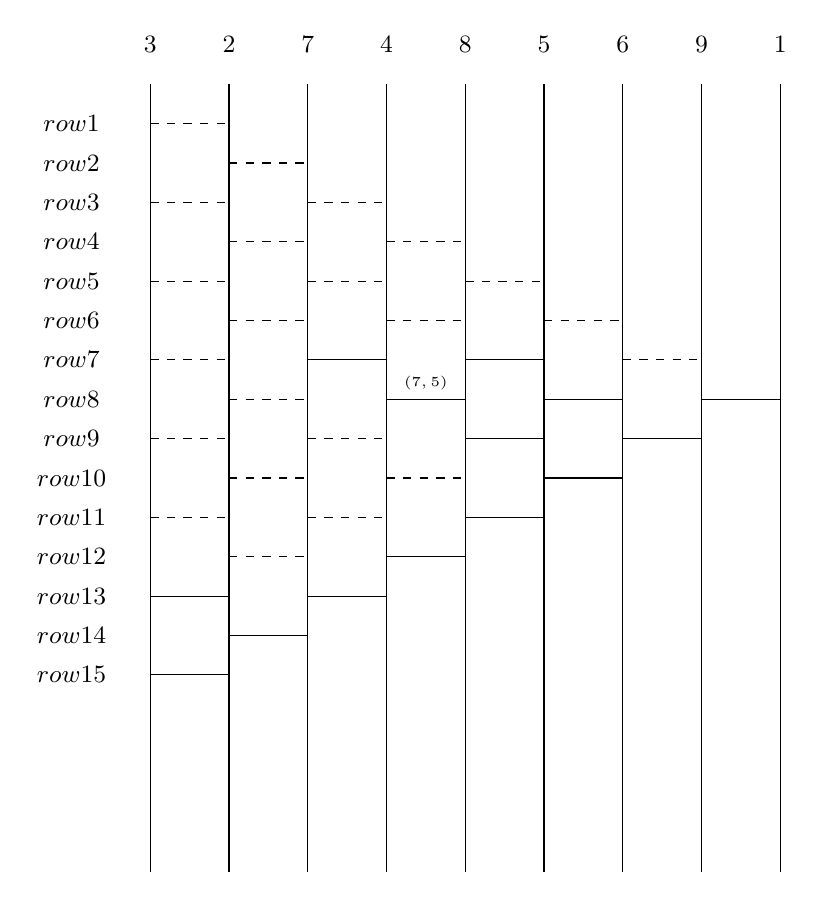
\begin{tikzpicture}
        \draw(0,0) to (0,10);
            \draw[dashed] (0, 9.5) -- (1, 9.5);
            \draw[dashed] (0, 8.5) -- (1, 8.5);
            \draw[dashed] (0, 7.5) -- (1, 7.5);
            \draw[dashed] (0, 6.5) -- (1, 6.5);
            \draw[dashed]         (0, 5.5) -- (1, 5.5);
            \draw[dashed]         (0, 4.5) -- (1, 4.5);
            \draw         (0, 3.5) to (1, 3.5);
            \draw         (0, 2.5) to (1, 2.5);
        \draw(1,0) to(1,10);
            \draw[dashed] (1, 9) -- (2, 9);
            \draw[dashed] (1, 8) -- (2, 8);
            \draw[dashed] (1, 7) -- (2, 7);
                
            \draw[dashed] (1, 6) -- (2, 6);
            \draw[dashed] (1, 5) -- (2, 5);
            \draw[dashed] (1, 4) -- (2, 4);
            \draw (1, 3) to (2, 3);
        \draw(2,0) to(2,10);
            \draw[dashed] (2, 8.5) -- (3, 8.5);
            \draw[dashed] (2, 7.5) -- (3, 7.5);
            \draw         (2, 6.5) to (3, 6.5);
            \draw[dashed] (2, 5.5) -- (3, 5.5);
            \draw[dashed] (2, 4.5) -- (3, 4.5);
            \draw         (2, 3.5) to (3, 3.5);
        \draw(3,0) to(3,10);
            \draw[dashed](3, 8) -- (4, 8);
            \draw[dashed](3, 7) -- (4, 7);
            \node at(3.5, 6.2){\tiny{$(7,5)$}};
            \draw        (3, 6) to (4, 6);
            \draw[dashed](3, 5) -- (4, 5);
            \draw        (3, 4) to (4, 4);
        \draw(4,0) to(4,10);
            \draw[dashed](4, 7.5) -- (5, 7.5);
            \draw(4, 6.5) to (5, 6.5);
            \draw(4, 5.5) to (5, 5.5);
            \draw(4, 4.5) to (5, 4.5);
        \draw(5,0) to(5,10);
            \draw[dashed](5, 7) -- (6, 7);
            \draw(5, 6) to (6, 6);
            \draw(5, 5) to (6, 5);
        \draw(6,0) to(6,10);
            \draw[dashed](6, 6.5) to (7, 6.5);
            \draw        (6, 5.5) to (7, 5.5);
        \draw(7,0) to(7,10);
            \draw(7, 6) to (8, 6);
        \draw(8,0) to(8,10);

        \node at(0, 10.5){\small{$3$}};
        \node at(1, 10.5){\small{$2$}};
        \node at(2, 10.5){\small{$7$}};
        \node at(3, 10.5){\small{$4$}};
        \node at(4, 10.5){\small{$8$}};
        \node at(5, 10.5){\small{$5$}};
        \node at(6, 10.5){\small{$6$}};
        \node at(7, 10.5){\small{$9$}};
        \node at(8, 10.5){\small{$1$}};

        \node at(-1, 9.5){\small{$row 1$}};
        \node at(-1, 9.0){\small{$row 2$}};
        \node at(-1, 8.5){\small{$row 3$}};
        \node at(-1, 8.0){\small{$row 4$}};
        \node at(-1, 7.5){\small{$row 5$}};
        \node at(-1, 7.0){\small{$row 6$}};
        \node at(-1, 6.5){\small{$row 7$}};
        \node at(-1, 6.0){\small{$row 8$}};
        \node at(-1, 5.5){\small{$row 9$}};
        \node at(-1, 5.0){\small{$row 10$}};
        \node at(-1, 4.5){\small{$row 11$}};
        \node at(-1, 4.0){\small{$row 12$}};
        \node at(-1, 3.5){\small{$row 13$}};
        \node at(-1, 3.0){\small{$row 14$}};
        \node at(-1, 2.5){\small{$row 15$}};
    \end{tikzpicture}
    \caption{Canonical ladder such that each bar or absence of a bar is calculated using the Equation~\ref{getCordEqn}.}
    \label{Fig:CanLArbitrary}
\end{figure}




\section{Locating the Bar for a Given Inversion in $CL((n,n-1, \dots 1))$}
In the previous section, we looked up a bar for a given inversion for some arbitrary permutation 
in $O(n)$ time. Clearly this is less than ideal. However, if $\pi$ is an arbitrary permutation 
of order $n$, we require linear time to calculate the location of a bar. 
In this section, we calculate the location of a bar corresponding to an inversion for $CL((n,n-1, \dots, 1))$ 
in $O(1)$ time. 
Let  $\pi=(n,n-1,n-2,...,1)$, then each associated diagonal in $CL(\pi)$ is fully occupied by bars. 
Let $x,y$ be a pair of elements in $\pi$ such that $x>y$ and $2 \leq x \leq n$. 
We know there exists a bar, $(x,y)$, in $CL((n,n-1, \dots 1))$ along the associated diagonal of $x$.
We compute the row and column of a bar $(x,y)$ in $CL((n,n-1, \dots 1))$ in $O(1)$ time using Equation~\ref{revCordEqn}. 
\begin{equation} \label{revCordEqn}
(row,column)=(2n-2x + (x-y), (x-y))
\caption{GetCoordinatesReverse}
\end{equation}

For example, given $\pi=(6,5,4,3,2,1)$, bar $(5,2)$ is located at row $5$; note that $5=(2n-2x)+(x-y)$. Bar $(5,2)$ is also located at column 
$3$; note that $3=x-y$. To see the canonical ladder for $(6,5,4,3,2,1)$ with the corresponding 
bars, please refer to Figure~\ref{Fig:RootLadderReverse}.
\begin{figure}[h]
    \centering
    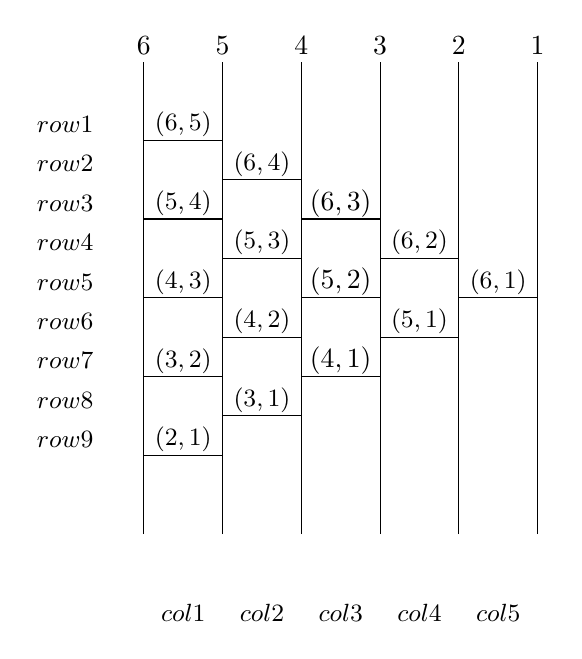
\begin{tikzpicture}
        \draw(0,0) to (0,6);
            \node at (0.5, 5.2){\small{$(6,5)$}};
            \draw(0, 5) to (1, 5);
            \node at (0.5, 4.2){\small{$(5,4)$}};
            \draw(0, 4) to (1, 4);
            \node at (0.5, 3.2){\small{$(4,3)$}};
            \draw(0, 3) to (1, 3);
            \node at (0.5, 2.2){\small{$(3,2)$}};
            \draw(0, 2) to (1, 2);
            \node at (0.5, 1.2){\small{$(2,1)$}};
            \draw(0, 1) to (1, 1);
        \draw(1,0) to (1,6);
            \node at(1.5, 4.7){\small{$(6,4)$}};
            \draw(1, 4.5) to (2, 4.5);
            \node at(1.5, 3.7){\small{$(5,3)$}};
            \draw(1, 3.5) to (2, 3.5);
            \node at(1.5, 2.7){\small{$(4,2)$}};
            \draw(1, 2.5) to (2, 2.5);
            \node at(1.5, 1.7){\small{$(3,1)$}};
            \draw(1, 1.5) to (2, 1.5);
        \draw(2,0) to (2,6);
            \node at(2.5, 4.2){$(6,3)$};
            \draw(2, 4) to (3, 4);
            \node at(2.5, 3.2){$(5,2)$};
            \draw(2, 3) to (3, 3);
            \node at(2.5, 2.2){$(4,1)$};
            \draw(2, 2) to (3, 2);
        \draw(3,0) to (3,6);
            \node at(3.5, 3.7){\small{$(6, 2)$}};
            \draw(3, 3.5) to (4, 3.5);
            \node at(3.5, 2.7){\small{$(5, 1)$}};
            \draw(3, 2.5) to (4, 2.5);
        \draw(4,0) to (4,6);
            \node at(4.5, 3.2){\small{$(6,1)$}};
            \draw(4, 3) to (5, 3);
        \draw(5,0) to (5,6);

        \node at(0, 6.2){$6$};
        \node at(1, 6.2){$5$};
        \node at(2, 6.2){$4$};
        \node at(3, 6.2){$3$};
        \node at(4, 6.2){$2$};
        \node at(5, 6.2){$1$};

        \node at(-1, 5.2){\small{$row 1$}};
        \node at(-1, 4.7){\small{$row 2$}};
        \node at(-1, 4.2){\small{$row 3$}};
        \node at(-1, 3.7){\small{$row 4$}};
        \node at(-1, 3.2){\small{$row 5$}};
        \node at(-1, 2.7){\small{$row 6$}};
        \node at(-1, 2.2){\small{$row 7$}};
        \node at(-1, 1.7){\small{$row 8$}};
        \node at(-1, 1.2){\small{$row 9$}};

        \node at(0.5, -1){\small{$col1$}};
        \node at(1.5, -1){\small{$col2$}};
        \node at(2.5, -1){\small{$col3$}};
        \node at(3.5, -1){\small{$col4$}};
        \node at(4.5, -1){\small{$col5$}};
    \end{tikzpicture}
    \caption{Canonical ladder for $(6,5,4,3,2,1)$. The location of each bar can be calculated using the formula $(2n-2x + (x-y), (x-y))$}
    \label{Fig:RootLadderReverse}
\end{figure}
We use Equation~\ref{revCordEqn} to locate a bar when we know $\pi=(n,n-1, \dots, 2,1)$. We use Equation~\ref{revCordEqn} when possible 
because the calculation time is $O(1)$ rather than $O(n)$. 


% in the corresponding $CL(\pi_{n})$. Further work is required to determine if removing bars from $CL(n,n-1, \dots, 1)$ 


\section{Algorithm: {\sc CreateCanonical}}
In this section we provide the data structure used to represent the canonical ladder in code. We then provide the algorithm for creating the canonical ladder corresponding to any permutation of 
order $n$. 
To create the canonical ladder 
we must represent the canonical ladder in code. We use Theorem~\ref{Theorem:RootHeight} and Corollary~\ref{Corollary:RootHeight} to prove the 
veracity of the representation of the canonical ladder.
 \begin{theorem}
   The number of rows required for the canonical ladder corresponding to the descending permutation of order $n$ is $2(n-1) - 1$.
   \label{Theorem:RootHeight}
 \end{theorem}
 \begin{proof}
 	Let $\pi$ be the descending permutation of order $n$. Let $route(x)$ be the route of $n \geq x \geq 2 \in \pi$. We know that 
     when $x=n$, $route(x)$ has $n-1$ bars, each requiring their own row. Thus, $CL((n,n-1, \dots, 1))$ requires at least $n-1$ rows. 
     For each subsequent $x$ from $[n-1 \dots 2]$, each $route(x)$ requires one more row to be added to $CL((n, n-1, \dots 1))$. 
     We get an additional $n-2$ rows added to $CL$, one for each $route([n-1 \geq x \geq 2])$. Therefore, the total number of rows is 
     $(n-1)+(n-2)=2(n-1)-1$.
 \end{proof}

 \begin{corollary}
     The upper bound for the number of rows of any canonical ladder of order $n$ is $2(n-1)-1$.
     \label{Corollary:RootHeight}
 \end{corollary}
 \begin{proof}
     By Theorem~\ref{Theorem:RootHeight}, we know that $2(n-1)-1$ is the number of rows required for 
     the canonical ladder corresponding 
     to the descending permutation of order $n$. By removing 
     bars from the canonical ladder for the descending permutation of order $n$, we can derive any other canonical ladder for any other permutation 
     of order $n$; removing a bar translates to removing an 
     inversion in $\pi$. Removing bars from the canonical ladder corresponding to the descending permutation of order $n$ 
     does not necessarily remove a row from the ladder, however, removing bars from the ladder certainly does not add any more rows 
     to $ladder$. Therefore, $2(n-1)-1$ is the upper bound for the number of rows required for any ladder of order $n$.
 \end{proof}
Using Theorem~\ref{Theorem:RootHeight} and Corollary~\ref{Corollary:RootHeight}, 
we represent a canonical ladder as a binary matrix with $2(n-1)-1$ rows and $n-1$ columns. Let $matrix[row][col]=1$ 
indicate a bar at the given row and column in the canonical ladder along an associated diagonal. Let $matrix[row][col]=0$ indicate the absence 
of a bar at the given row and column in the canonical ladder along an associated diagonal. Let $matrix[row][col]=-$ indicate irrelevancy as to whether 
a $1$ or $0$ is at the given row and column because the row and column do not lie on an associated diagonal. To see the canonical ladder for 
$(4,2,1,3)$ and the corresponding binary matrix, refer to Figure~\ref{Fig:MatrixLadder}.
\begin{figure}[ht]
    \begin{minipage}{.4\textwidth}
        \centering
        \begin{tikzpicture}
        \node at(0, 4.2){\small{$4$}};
        \node at(1, 4.2){\small{$2$}};
        \node at(2, 4.2){\small{$1$}};
        \node at(3, 4.2){\small{$3$}};
        \draw(0, 0) to (0, 4);
            \draw(0,3.9) to (1,3.9);
            \draw[dashed](0,1.9) -- (1,1.9);
            \draw(0,0.1) to (1,0.1);
        \draw(1, 0) to (1, 4);
            \draw(1,2.9) to (2,2.9);
            \draw[dashed](1,0.9) -- (2,0.9);
        \draw(2, 0) to (2, 4);
            \draw(2,1.9) to (3,1.9);
        \draw(3, 0) to (3, 4);
        \end{tikzpicture}
    \end{minipage}
    \begin{minipage}{0.4\textwidth}
        \begin{flushright}
        \begin{bmatrix}
            1 & - & - \\
            - & 1 & -\\
            0 & - & 1 \\ 
            - & 0 & - \\
            1 & - & - \\

        \end{bmatrix}
    \end{flushright}
    \end{minipage}
    \caption{Canonical ladder and corresponding binary matrix.}
    \label{Fig:MatrixLadder}
\end{figure}

Using Equation~\ref{getCordEqn}, and the binary matrix representation 
of a ladder, we define algorithm {\sc CreateCanonical} which can be found 
in Algorithm~\ref{Alg:RootLadder} to create the canonical ladder for 
any given permutation of order $n$. 
The initial conditions of {\sc CreateCanonical} are the 
following. Let $ladder$ be the binary matrix representing $CL(\pi)$ initialized to $-$. Let $\pi$ be an arbitrary permutation 
of order $n$. Let $x$ be the currently maximal element in $\pi$, initialized to $n$. Let {\sc GetCoordinates} refer to 
Equation~\ref{getCordEqn}. 
\begin{algorithm}[ht]
	\begin{algorithmic}[1]
		\Function {CreateCanonical}{$ladder$, $\pi$, $x$}
			\While{$x>1$}
                \State $pos(x) \gets $ index of $x \in \pi$
                \For{$i$ \textbf{from} $1$  \textbf{to} $x$}
                    \If{$i \neq pos(x)$}
                        
                        \State $(row, column) \gets${\sc GetCoordinates($x$, $pos(x), i$)}
                        \If{$pos(x)<i$}
                            \State $ladder[row][col] \gets 1$
                        \Else
                            \State $ladder[row][col] \gets 0$
                        \EndIf
                    \EndIf
                \EndFor
                \State $\pi \gets \pi - x$
                \State $x \gets x-1$
            \EndWhile
        \EndFunction

	\end{algorithmic}
	\caption{The algorithm for creating the canonical ladder of $OptL\{\pi\}$}
	\label{Alg:RootLadder}
\end{algorithm}

On each iteration of the while loop, all $x-1$ $1s$ and $0s$  along the associated diagonal of the $xth$ 
element are added to $ladder$ within the for-loop. {\sc GetCoordinates}, which refers to Equation~\ref{getCordEqn}, 
returns the row and column coordinate for the respective $1$ or $0$ for the pair of elements, $x>y$. Note that we call {\sc GetCoordinates} with 
the arguments $(x,pos(x),i)$. When referring to Equation~\ref{getCordEqn} the variables 
are $(x,pos'(x),pos'(y))$. Prior to the next iteration of the while loop, 
$x$ is removed from $\pi$ and all elements to the right of $x$ are moved to the left by one index. 
Then, $x$ is decremented by $1$. The while loop continues until $x=1$. Determining $pos(x)$ 
is done in $O(x)$ time. Removing $x$ from $\pi$ is done in $O(x)$ time. Calculating the row and column 
for each $(x,y)$ is done in $O(1)$ time. Overall, the algorithms complexity is $O(n^2)$.
We also note that {\sc CreateCanonical} creates the ladder representation with clean level $1$.  
Given three elements, $x>y>z$ and $pos(x) < pos(y) < pos(z)$, Equation~\ref{getCordEqn} returns a lesser row 
for $(x,z)$ than for $(y,z)$. Therefore, {\sc CreateCanonical} creates a representation of a ladder with clean level $1$. 
To see the resulting state of the ladder for each iteration of {\sc CreateCanonical} with $(5,7,3,4,1,2,6)$ please refer to Figure~\ref{Fig:CreateRoot}. 
\begin{figure}[t]
    \centering 
    \begin{minipage}{.3\textwidth}
    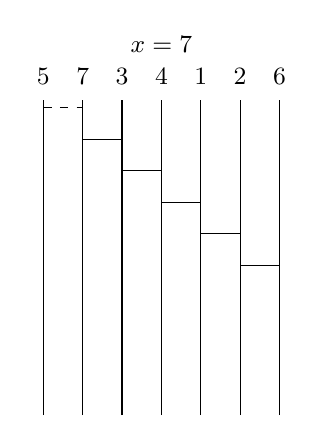
\begin{tikzpicture}
        \draw(0, 0) to (0, 4);
        
        \draw(.5, 0) to (.5, 4);
        \draw(1, 0) to (1, 4);
        \draw(1.5, 0) to (1.5, 4);
        \draw(2, 0) to (2, 4);
        \draw(2.5, 0) to (2.5, 4);
        \draw(3, 0) to (3, 4);
        
        \draw(2.5, 1.9) to (3, 1.9);
        \draw(2.0, 2.3) to (2.5, 2.3);
        \draw(1.5, 2.7) to (2.0, 2.7);
        \draw(1.0, 3.1) to (1.5, 3.1);
        \draw(0.5, 3.5) to (1.0, 3.5);

        \draw[dashed] (0, 3.9) -- (0.5, 3.9);
        \node at(1.5, 4.7){\small{$x=7$}};
        \node at(0, 4.3){\small{$5$}};
        \node at(.5, 4.3){\small{$7$}};
        \node at(1, 4.3){\small{$3$}};
        \node at(1.5, 4.3){\small{$4$}};
        \node at(2, 4.3){\small{$1$}};
        \node at(2.5, 4.3){\small{$2$}};
        \node at(3, 4.3){\small{$6$}};
    \end{tikzpicture}
    \end{minipage}
    \begin{minipage}{.3\textwidth}
    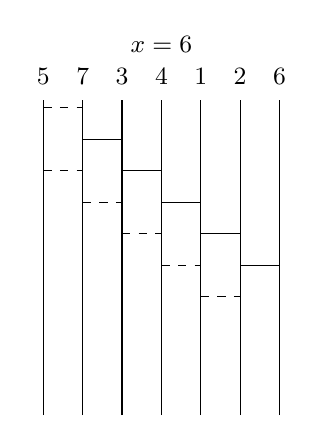
\begin{tikzpicture}
        \draw(0, 0) to (0, 4);
        \draw(.5, 0) to (.5, 4);
        \draw(1, 0) to (1, 4);
        \draw(1.5, 0) to (1.5, 4);
        \draw(2, 0) to (2, 4);
        \draw(2.5, 0) to (2.5, 4);
        \draw(3, 0) to (3, 4);
        
        \draw[dashed] (0, 3.9) -- (0.5, 3.9);
        \draw[dashed] (2, 1.5) -- (2.5, 1.5);
        \draw[dashed] (1.5, 1.9) -- (2.0, 1.9);
        \draw[dashed] (1.0, 2.3) -- (1.5, 2.3);
        \draw[dashed] (0.5, 2.7) -- (1.0, 2.7);
        \draw[dashed] (0.0, 3.1) -- (0.5, 3.1);
        \draw(2.5, 1.9) to (3, 1.9);
        \draw(2.0, 2.3) to (2.5, 2.3);
        \draw(1.5, 2.7) to (2.0, 2.7);
        \draw(1.0, 3.1) to (1.5, 3.1);
        \draw(0.5, 3.5) to (1.0, 3.5);

        \node at(1.5, 4.7){\small{$x=6$}};

        \node at(0, 4.3){\small{$5$}};
        \node at(.5, 4.3){\small{$7$}};
        \node at(1, 4.3){\small{$3$}};
        \node at(1.5, 4.3){\small{$4$}};
        \node at(2, 4.3){\small{$1$}};
        \node at(2.5, 4.3){\small{$2$}};
        \node at(3, 4.3){\small{$6$}};
    \end{tikzpicture}
    \end{minipage}
   \begin{minipage}{.3\textwidth}
    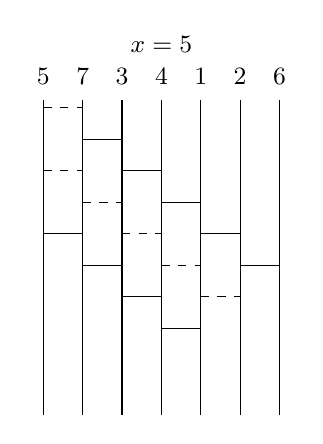
\begin{tikzpicture}
        \draw(0, 0) to (0, 4);
            \draw(0, 2.3) to (0.5, 2.3);
        \draw(.5, 0) to (.5, 4);
            \draw(.5, 1.9) to (1, 1.9);
        \draw(1, 0) to (1, 4);
            \draw(1, 1.5) to (1.5, 1.5);
        \draw(1.5, 0) to (1.5, 4);
            \draw(1.5, 1.1) to (2, 1.1);
            \draw(1.5, 2.7) to (2, 2.7);
        \draw(2, 0) to (2, 4);
        \draw(2.5, 0) to (2.5, 4);
        \draw(3, 0) to (3, 4);
      


        \draw(2.5, 1.9) to (3, 1.9);
        \draw(2.0, 2.3) to (2.5, 2.3);

        \draw(1.0, 3.1) to (1.5, 3.1);
        \draw(0.5, 3.5) to (1.0, 3.5);
      
        \draw[dashed] (0, 3.9) -- (0.5, 3.9);
        \draw[dashed] (2, 1.5) -- (2.5, 1.5);
        \draw[dashed] (1.5, 1.9) -- (2.0, 1.9);
        \draw[dashed] (1.0, 2.3) -- (1.5, 2.3);
        \draw[dashed] (0.5, 2.7) -- (1.0, 2.7);
        \draw[dashed] (0.0, 3.1) -- (0.5, 3.1);
        

        \node at(1.5, 4.7){\small{$x=5$}};
        \node at(0, 4.3){\small{$5$}};
        \node at(.5, 4.3){\small{$7$}};
        \node at(1, 4.3){\small{$3$}};
        \node at(1.5, 4.3){\small{$4$}};
        \node at(2, 4.3){\small{$1$}};
        \node at(2.5, 4.3){\small{$2$}};
        \node at(3, 4.3){\small{$6$}};
    \end{tikzpicture}
    \end{minipage}
        
    \begin{minipage}{.3\textwidth}
    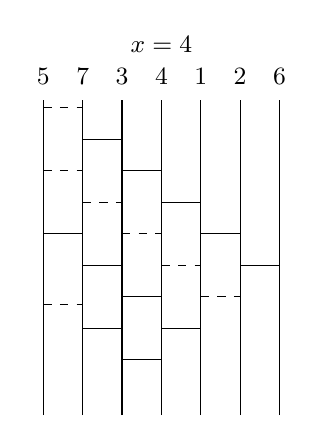
\begin{tikzpicture}
    \draw(0, 0) to (0, 4);
            \draw(0, 2.3) to (0.5, 2.3);
        \draw(.5, 0) to (.5, 4);
            \draw(.5, 1.9) to (1, 1.9);
            \draw(0.5, 1.1) to (1, 1.1);
        \draw(1, 0) to (1, 4);
            \draw(1, 1.5) to (1.5, 1.5);
            \draw(1, 0.7) to (1.5, 0.7);
        \draw(1.5, 0) to (1.5, 4);
            \draw(1.5, 1.1) to (2, 1.1);
            \draw(1.5, 2.7) to (2, 2.7);
        \draw(2, 0) to (2, 4);
        \draw(2.5, 0) to (2.5, 4);
        \draw(3, 0) to (3, 4);
        

        \draw(2.5, 1.9) to (3, 1.9);
        \draw(2.0, 2.3) to (2.5, 2.3);

        \draw(1.0, 3.1) to (1.5, 3.1);
        \draw(0.5, 3.5) to (1.0, 3.5);
      
        \draw[dashed] (0, 3.9) -- (0.5, 3.9);
        \draw[dashed] (2, 1.5) -- (2.5, 1.5);
        \draw[dashed] (1.5, 1.9) -- (2.0, 1.9);
        \draw[dashed] (1.0, 2.3) -- (1.5, 2.3);
        \draw[dashed] (0.5, 2.7) -- (1.0, 2.7);
        \draw[dashed] (0.0, 3.1) -- (0.5, 3.1);
        \draw[dashed] (0.0, 1.4) -- (0.5, 1.4);
        

        \node at(1.5, 4.7){\small{$x=4$}};
        \node at(0, 4.3){\small{$5$}};
        \node at(.5, 4.3){\small{$7$}};
        \node at(1, 4.3){\small{$3$}};
        \node at(1.5, 4.3){\small{$4$}};
        \node at(2, 4.3){\small{$1$}};
        \node at(2.5, 4.3){\small{$2$}};
        \node at(3, 4.3){\small{$6$}};
    \end{tikzpicture}
    \end{minipage}
    \begin{minipage}{.3\textwidth}
    \begin{tikzpicture}
     \draw(0, 0) to (0, 4);
            \draw(0, 2.3) to (0.5, 2.3);
            \draw(0, 0.7) to (0.5, 0.7);
        \draw(.5, 0) to (.5, 4);
            \draw(.5, 1.9) to (1, 1.9);
            \draw(0.5, 1.1) to (1, 1.1);
            \draw(0.5, 0.3) to (1, 0.3);
        \draw(1, 0) to (1, 4);
            \draw(1, 1.5) to (1.5, 1.5);
            \draw(1, 0.7) to (1.5, 0.7);
        \draw(1.5, 0) to (1.5, 4);
            \draw(1.5, 1.1) to (2, 1.1);
            \draw(1.5, 2.7) to (2, 2.7);
        \draw(2, 0) to (2, 4);
        \draw(2.5, 0) to (2.5, 4);
        \draw(3, 0) to (3, 4);
       

        \draw(2.5, 1.9) to (3, 1.9);
        \draw(2.0, 2.3) to (2.5, 2.3);

        \draw(1.0, 3.1) to (1.5, 3.1);
        \draw(0.5, 3.5) to (1.0, 3.5);
      
        \draw[dashed] (0, 3.9) -- (0.5, 3.9);
        \draw[dashed] (2, 1.5) -- (2.5, 1.5);
        \draw[dashed] (1.5, 1.9) -- (2.0, 1.9);
        \draw[dashed] (1.0, 2.3) -- (1.5, 2.3);
        \draw[dashed] (0.5, 2.7) -- (1.0, 2.7);
        \draw[dashed] (0.0, 3.1) -- (0.5, 3.1);
        \draw[dashed] (0.0, 1.4) -- (0.5, 1.4);
        

        \node at(1.5, 4.7){\small{$x=3$}};
        \node at(0, 4.3){\small{$5$}};
        \node at(.5, 4.3){\small{$7$}};
        \node at(1, 4.3){\small{$3$}};
        \node at(1.5, 4.3){\small{$4$}};
        \node at(2, 4.3){\small{$1$}};
        \node at(2.5, 4.3){\small{$2$}};
        \node at(3, 4.3){\small{$6$}};
    \end{tikzpicture}
    \end{minipage}
    \begin{minipage}{.3\textwidth}
   \begin{tikzpicture}
     \draw(0, 0) to (0, 4);
            \draw(0, 2.3) to (0.5, 2.3);
            \draw(0, 0.7) to (0.5, 0.7);
        \draw(.5, 0) to (.5, 4);
            \draw(.5, 1.9) to (1, 1.9);
            \draw(0.5, 1.1) to (1, 1.1);
            \draw(0.5, 0.3) to (1, 0.3);
        \draw(1, 0) to (1, 4);
            \draw(1, 1.5) to (1.5, 1.5);
            \draw(1, 0.7) to (1.5, 0.7);
        \draw(1.5, 0) to (1.5, 4);
            \draw(1.5, 1.1) to (2, 1.1);
            \draw(1.5, 2.7) to (2, 2.7);
        \draw(2, 0) to (2, 4);
        \draw(2.5, 0) to (2.5, 4);
        \draw(3, 0) to (3, 4);
      


        \draw(2.5, 1.9) to (3, 1.9);
        \draw(2.0, 2.3) to (2.5, 2.3);

        \draw(1.0, 3.1) to (1.5, 3.1);
        \draw(0.5, 3.5) to (1.0, 3.5);
      
        \draw[dashed] (0, 3.9) -- (0.5, 3.9);
        \draw[dashed] (2, 1.5) -- (2.5, 1.5);
        \draw[dashed] (1.5, 1.9) -- (2.0, 1.9);
        \draw[dashed] (1.0, 2.3) -- (1.5, 2.3);
        \draw[dashed] (0.5, 2.7) -- (1.0, 2.7);
        \draw[dashed] (0.0, 3.1) -- (0.5, 3.1);
        \draw[dashed] (0.0, 1.4) -- (0.5, 1.4);
        \draw[dashed] (0.0, 0.1) -- (0.5,0.1);
        

        \node at(1.5, 4.7){\small{$x=2$}};
        \node at(0, 4.3){\small{$5$}};
        \node at(.5, 4.3){\small{$7$}};
        \node at(1, 4.3){\small{$3$}};
        \node at(1.5, 4.3){\small{$4$}};
        \node at(2, 4.3){\small{$1$}};
        \node at(2.5, 4.3){\small{$2$}};
        \node at(3, 4.3){\small{$6$}};

    \end{tikzpicture}
    \end{minipage}
    

        
        % \node at(9.5, -5.3){\small{$x=2,row=10$}};

        % \node at(0, -.7){\small{$5$}};
        % \node at(.5, -.7){\small{$7$}};
        % \node at(1, -.7){\small{$3$}};
        % \node at(1.5, -.7){\small{$4$}};
        % \node at(2, -.7){\small{$1$}};
        % \node at(2.5, -.7){\small{$2$}};
        % \node at(3, -.7){\small{$6$}};
        
        % \node at(4, -.7){\small{$5$}};
        % \node at(4.5, -.7){\small{$7$}};
        % \node at(5, -.7){\small{$3$}};
        % \node at(5.5, -.7){\small{$4$}};
        % \node at(6, -.7){\small{$1$}};
        % \node at(6.5, -.7){\small{$2$}};
        % \node at(7, -.7){\small{$6$}};

        % \node at(8, -.7){\small{$5$}};
        % \node at(8.5, -.7){\small{$7$}};
        % \node at(9, -.7){\small{$3$}};
        % \node at(9.5, -.7){\small{$4$}};
        % \node at(10, -.7){\small{$1$}};
        % \node at(10.5, -.7){\small{$2$}};
        % \node at(11, -.7){\small{$6$}};
        
    
    \caption{The ordering of the state of the ladder when creating the root ladder for $(5,7,3,4,1,2,6)$}
    \label{Fig:CreateRoot}
\end{figure}

% \begin{lemma}
% 	The time complexity for CreateRoot is $O(n^{2})$
% \end{lemma}
% \begin{proof}
% 	The for-loop runs from some arbitrary index to $n$ on each function call. Thus, we get $O(n)$. The following 
%     recursion holds, $CreateRoot(n-k) = CreateRoot((n-k)+1) + n=CreateRoot((n-k)+2) + n-1\dots $. The recurrence 
%     relation is reduced to $n(n+1)/2= O(n^2)$.
% \end{proof}

A main contribution of this thesis is the canonical ladder and the algorithm {\sc CreateCanonical}.
By defining the canonical ladder we are able to list all $n!$ canonical ladders in any order. 
Let $L_{n}$ be the set of all $n!$ canonical ladders. 
\begin{lemma}
    Using {\sc CreateCanonical}, we can list $L_{n}$ in any order.
\end{lemma}
\begin{proof}
 Let $S_{n}$ be the set of all permutations of order $n$. We simply apply an ordering to list $S_{n}$. For each 
 permutation in $S_{n}$, we apply {\sc CreateCanonical}, thus listing $L_{n}$ in the same order as $S_{n}$.
\end{proof}
We create each $CL(\pi)$ in $O(n^2)$ time using {\sc CreateCanonical}. However, using {\sc CreateCanonical} to list $L_{n}$ is inefficient, 
seeing as each ladder is created in $O(n^2)$ time. 
In chapters 4 and 5 we provide two Gray code listing algorithms, {\sc ModifiedSJT} and {\sc ListLnByKBars}, to list $L_{n}$ in constant amortized time. 
The details of these algorithms are found in chapters 4 and 5 respectively.  
% {\sc ModifiedSJT} and {\sc CyclicBar} require additional auxiliary functions. We define {\sc Inv(x)} as follows: $|\forall y \in \pi : y < x, p_{y}>p_{x}|$. 
% For example, given $(3,4,1,5,6,2)$, {\sc Inv(1)=0}, {\sc Inv(2)=0}, {\sc Inv(3)=2}, {\sc Inv(4)=2}, {\sc Inv(5)=1}, {\sc Inv(6)=1}. 
% Given {\sc Inv(x)}, 
% we can define the function {\sc GetCoordinates2}. In order to define {\sc GetCoordinates2}, let $x>y \in \pi$. Given 
% $p_{x}$ and $p_{y}$, suppose a transposition were applied to $x$ and $y$. Prior to the transposition 
% of $x$ and $y$, if $p_{x} = p_{y}-1$ then {\sc GetCoordinates2} returns the row and column of the bar $(x,y)$ to be removed 
% from the ladder. If $p_{x}=p_{y}+1$, then {\sc GetCoordinates} returns 
% the row and column of bar $(x,y)$ to be added to the ladder. 








\section{Procedure}

So far, the problem has been introduced and the required terminology has been defined. In the procedure section,
 the details of {\sc ModifiedSJT} and {\sc CyclicBar} are provided. These details include the pseudocode for 
 each of the algorithms, the initial conditions for each of the algorithms, the structures produced by each 
 of the algorithms, and a number of lemmas and proofs for each of the two algorithms. In the procedure section, 
 the algorithms are assessed independently of each other.
%%section SJT
\subsection{The Modified Steinhaus-Johnson-Trotter Algorithm}

For the initial conditions of {\sc ModifiedSJT} assume the following. 
Let be the $ladder$ be initialized a two dimensional binary array of only $0's$.
 Let a $1$ at $row=i,col=j$ 
indicate a bar at  $row=i,col=j$. Let a $0$ at $row=i,col=j$ 
indicate the absence of a bar at  $row=i,col=j$.
Let $n$ be the maximum element. Let $direction$ be a one 
indexed array set to left for all indexes. Let left indicate that a bar is to be added to the ladder; bars 
are added left to right. Let right indicate a bar is to be removed from the ladder; bars 
are removed right to left. Let $route$ be initialized to $2$. On each recursive call 
$route$ is incremented by $1$ from $2,3 \dots n$.
\begin{algorithm}
  \begin{algorithmic}[1]
    \Function{ModifiedSJT}{$n$, $ladder$, $route$, $direction$}
     %%base case
      \If{$route > n$}
        \State {\sc print}($ladder$)
        \State \textbf{return}
      \EndIf
      %%swap the nth element n-1 times
      \For{$i$ \textbf{from} $0$ \textbf{to} $route-1$}
        \If{$i = 0$}
          \State {\sc ModifiedSJT}($n$, $ladder$, $route+1$, $direction$)
        \Else 
          \If{$direction[route]=$ left}
            \State $row \gets (n) + (n - route) - (i);$
            \State $col \gets route - i$
            \State $ladder[row][col] \gets 1$
          \Else
            \State $col \gets i$
            \State $row \gets 2(n - route) + (i)$
            \State $ladder[row][col] \gets 0$
          \EndIf
        \EndIf
        \State {\sc ModifiedSJT}($n$, $ladder$, $route+1$, $direction$)
      \EndFor
      \If{$direction[route] =$ left}
        \State $direction[route] \gets$ right
      \Else
        \State $direction[route] \gets$ left
      \EndIf
    \EndFunction
  \end{algorithmic}
  \caption{Modification of the {\sc SJT} algorithm for listing $L_{n}$}
  \label{Alg:ModSJT}
\end{algorithm}


\pagebreak


The principles of the algorithm are the following. Given $route=k$, add or remove a bar for route $k$, then add or remove 
all bars for $route=k+1$. Once all bars for route $k+1$ have been added or removed, 
proceed to add or remove the next bar from $route=k$. Repeat until all $k-1$ bars have been added or removed from route $k$.
If $direction[route]$ is left, then bars of $route$ will be added to 
$ladder$ from right to left, bottom to top, until no more bars to $route$ can be added.
If $direction[route]$ is right, then bars will be removed from $ladder$, right to left, top to bottom, until 
no more bars from $route$ can be removed. Once all the bars for $route$ have 
been added or removed, then $direction[route]$ is reversed,
indicating that the opposite operation will be applied to the bars of the route when 
$route$ is next processed. The maximum number of bars for a given $route=k$ is $k-1$ and the minimum number of 
bars is $1$. On each recursive call, $route$ is 
incremented by $1$. When $route$ is greater than $n$, print the ladder 
and return. 


\begin{lemma}
  {\sc ModifiedSJT} produces $L_{n}$
\end{lemma}
\begin{proof}
  Since the algorithm is a modification of the Steinhaus-Johnson-Trotter algorithm, a similar proof for the SJT algorithm 
can be applied to the {\sc ModifiedSJT} algorithm. Suppose we want to list all $n!$ ladders 
of order $n$. Suppose we have all $n-1!$ ladders of order $n-1$, then for 
each ladder of order $n-1$ add a new column to the right; this results in $n-1$ columns seeing as 
the number of columns is one less than the number of elements. For each of the $n-1!$ ladders with $n-1$ columns 
add $0 \dots n-1$ bars beginning at column $n-1$ and ending 
at column $1$. Doing so results in $(n-1)!n=n!$ ladders of order $n$. To see 
an example of the proof please refer to Figure~\ref{Fig:CanLSJT}.
\end{proof}
%%prove the dimensions of the datastructure
\begin{center}
 \begin{figure}[!htp]
  \centering
  \begin{tikzpicture}
\draw(0.00,5.90) to (0.00,7.10);
\draw(0.20,5.90) to (0.20,7.10);
\draw(0.40,5.90) to (0.40,7.10);
\draw(0.60,5.90) to (0.60,7.10);


\draw(1.00,5.90) to (1.00,7.10);
\draw(1.20,5.90) to (1.20,7.10);
\draw(1.40,5.90) to (1.40,7.10);
\draw(1.60,5.90) to (1.60,7.10);
\draw(1.40, 6.60) to (1.60, 6.60);


\draw(2.00,5.90) to (2.00,7.10);
\draw(2.20,5.90) to (2.20,7.10);
\draw(2.40,5.90) to (2.40,7.10);
\draw(2.60,5.90) to (2.60,7.10);
\draw(2.20, 6.80) to (2.40, 6.80);
\draw(2.40, 6.60) to (2.60, 6.60);


\draw(3.00,5.90) to (3.00,7.10);
\draw(3.20,5.90) to (3.20,7.10);
\draw(3.40,5.90) to (3.40,7.10);
\draw(3.60,5.90) to (3.60,7.10);
\draw(3.00, 7.00) to (3.20, 7.00);
\draw(3.20, 6.80) to (3.40, 6.80);
\draw(3.40, 6.60) to (3.60, 6.60);


\draw(4.00,5.90) to (4.00,7.10);
\draw(4.20,5.90) to (4.20,7.10);
\draw(4.40,5.90) to (4.40,7.10);
\draw(4.60,5.90) to (4.60,7.10);
\draw(4.00, 7.00) to (4.20, 7.00);
\draw(4.20, 6.80) to (4.40, 6.80);
\draw(4.40, 6.60) to (4.60, 6.60);
\draw(4.20, 6.40) to (4.40, 6.40);


\draw(5.00,5.90) to (5.00,7.10);
\draw(5.20,5.90) to (5.20,7.10);
\draw(5.40,5.90) to (5.40,7.10);
\draw(5.60,5.90) to (5.60,7.10);
\draw(5.20, 6.80) to (5.40, 6.80);
\draw(5.40, 6.60) to (5.60, 6.60);
\draw(5.20, 6.40) to (5.40, 6.40);


\draw(0.00,4.40) to (0.00,5.60);
\draw(0.20,4.40) to (0.20,5.60);
\draw(0.40,4.40) to (0.40,5.60);
\draw(0.60,4.40) to (0.60,5.60);
\draw(0.40, 5.10) to (0.60, 5.10);
\draw(0.20, 4.90) to (0.40, 4.90);


\draw(1.00,4.40) to (1.00,5.60);
\draw(1.20,4.40) to (1.20,5.60);
\draw(1.40,4.40) to (1.40,5.60);
\draw(1.60,4.40) to (1.60,5.60);
\draw(1.20, 4.90) to (1.40, 4.90);


\draw(2.00,4.40) to (2.00,5.60);
\draw(2.20,4.40) to (2.20,5.60);
\draw(2.40,4.40) to (2.40,5.60);
\draw(2.60,4.40) to (2.60,5.60);
\draw(2.00, 5.10) to (2.20, 5.10);
\draw(2.20, 4.90) to (2.40, 4.90);


\draw(3.00,4.40) to (3.00,5.60);
\draw(3.20,4.40) to (3.20,5.60);
\draw(3.40,4.40) to (3.40,5.60);
\draw(3.60,4.40) to (3.60,5.60);
\draw(3.00, 5.10) to (3.20, 5.10);
\draw(3.40, 5.10) to (3.60, 5.10);
\draw(3.20, 4.90) to (3.40, 4.90);


\draw(4.00,4.40) to (4.00,5.60);
\draw(4.20,4.40) to (4.20,5.60);
\draw(4.40,4.40) to (4.40,5.60);
\draw(4.60,4.40) to (4.60,5.60);
\draw(4.20, 5.30) to (4.40, 5.30);
\draw(4.00, 5.10) to (4.20, 5.10);
\draw(4.40, 5.10) to (4.60, 5.10);
\draw(4.20, 4.90) to (4.40, 4.90);


\draw(5.00,4.40) to (5.00,5.60);
\draw(5.20,4.40) to (5.20,5.60);
\draw(5.40,4.40) to (5.40,5.60);
\draw(5.60,4.40) to (5.60,5.60);
\draw(5.00, 5.50) to (5.20, 5.50);
\draw(5.20, 5.30) to (5.40, 5.30);
\draw(5.00, 5.10) to (5.20, 5.10);
\draw(5.40, 5.10) to (5.60, 5.10);
\draw(5.20, 4.90) to (5.40, 4.90);


\draw(0.00,2.90) to (0.00,4.10);
\draw(0.20,2.90) to (0.20,4.10);
\draw(0.40,2.90) to (0.40,4.10);
\draw(0.60,2.90) to (0.60,4.10);
\draw(0.00, 4.00) to (0.20, 4.00);
\draw(0.20, 3.80) to (0.40, 3.80);
\draw(0.00, 3.60) to (0.20, 3.60);
\draw(0.40, 3.60) to (0.60, 3.60);
\draw(0.20, 3.40) to (0.40, 3.40);
\draw(0.00, 3.20) to (0.20, 3.20);


\draw(1.00,2.90) to (1.00,4.10);
\draw(1.20,2.90) to (1.20,4.10);
\draw(1.40,2.90) to (1.40,4.10);
\draw(1.60,2.90) to (1.60,4.10);
\draw(1.20, 3.80) to (1.40, 3.80);
\draw(1.00, 3.60) to (1.20, 3.60);
\draw(1.40, 3.60) to (1.60, 3.60);
\draw(1.20, 3.40) to (1.40, 3.40);
\draw(1.00, 3.20) to (1.20, 3.20);


\draw(2.00,2.90) to (2.00,4.10);
\draw(2.20,2.90) to (2.20,4.10);
\draw(2.40,2.90) to (2.40,4.10);
\draw(2.60,2.90) to (2.60,4.10);
\draw(2.00, 3.60) to (2.20, 3.60);
\draw(2.40, 3.60) to (2.60, 3.60);
\draw(2.20, 3.40) to (2.40, 3.40);
\draw(2.00, 3.20) to (2.20, 3.20);


\draw(3.00,2.90) to (3.00,4.10);
\draw(3.20,2.90) to (3.20,4.10);
\draw(3.40,2.90) to (3.40,4.10);
\draw(3.60,2.90) to (3.60,4.10);
\draw(3.00, 3.60) to (3.20, 3.60);
\draw(3.20, 3.40) to (3.40, 3.40);
\draw(3.00, 3.20) to (3.20, 3.20);


\draw(4.00,2.90) to (4.00,4.10);
\draw(4.20,2.90) to (4.20,4.10);
\draw(4.40,2.90) to (4.40,4.10);
\draw(4.60,2.90) to (4.60,4.10);
\draw(4.20, 3.40) to (4.40, 3.40);
\draw(4.00, 3.20) to (4.20, 3.20);


\draw(5.00,2.90) to (5.00,4.10);
\draw(5.20,2.90) to (5.20,4.10);
\draw(5.40,2.90) to (5.40,4.10);
\draw(5.60,2.90) to (5.60,4.10);
\draw(5.40, 3.60) to (5.60, 3.60);
\draw(5.20, 3.40) to (5.40, 3.40);
\draw(5.00, 3.20) to (5.20, 3.20);


\draw(0.00,1.40) to (0.00,2.60);
\draw(0.20,1.40) to (0.20,2.60);
\draw(0.40,1.40) to (0.40,2.60);
\draw(0.60,1.40) to (0.60,2.60);
\draw(0.20, 2.30) to (0.40, 2.30);
\draw(0.40, 2.10) to (0.60, 2.10);
\draw(0.20, 1.90) to (0.40, 1.90);
\draw(0.00, 1.70) to (0.20, 1.70);


\draw(1.00,1.40) to (1.00,2.60);
\draw(1.20,1.40) to (1.20,2.60);
\draw(1.40,1.40) to (1.40,2.60);
\draw(1.60,1.40) to (1.60,2.60);
\draw(1.00, 2.50) to (1.20, 2.50);
\draw(1.20, 2.30) to (1.40, 2.30);
\draw(1.40, 2.10) to (1.60, 2.10);
\draw(1.20, 1.90) to (1.40, 1.90);
\draw(1.00, 1.70) to (1.20, 1.70);


\draw(2.00,1.40) to (2.00,2.60);
\draw(2.20,1.40) to (2.20,2.60);
\draw(2.40,1.40) to (2.40,2.60);
\draw(2.60,1.40) to (2.60,2.60);
\draw(2.00, 2.50) to (2.20, 2.50);
\draw(2.20, 2.30) to (2.40, 2.30);
\draw(2.40, 2.10) to (2.60, 2.10);
\draw(2.00, 1.70) to (2.20, 1.70);


\draw(3.00,1.40) to (3.00,2.60);
\draw(3.20,1.40) to (3.20,2.60);
\draw(3.40,1.40) to (3.40,2.60);
\draw(3.60,1.40) to (3.60,2.60);
\draw(3.20, 2.30) to (3.40, 2.30);
\draw(3.40, 2.10) to (3.60, 2.10);
\draw(3.00, 1.70) to (3.20, 1.70);


\draw(4.00,1.40) to (4.00,2.60);
\draw(4.20,1.40) to (4.20,2.60);
\draw(4.40,1.40) to (4.40,2.60);
\draw(4.60,1.40) to (4.60,2.60);
\draw(4.40, 2.10) to (4.60, 2.10);
\draw(4.00, 1.70) to (4.20, 1.70);


\draw(5.00,1.40) to (5.00,2.60);
\draw(5.20,1.40) to (5.20,2.60);
\draw(5.40,1.40) to (5.40,2.60);
\draw(5.60,1.40) to (5.60,2.60);
\draw(5.00, 1.70) to (5.20, 1.70);






\end{tikzpicture}
  \caption{$L_{4}$ generated by the {\sc ModifiedSJT} algorithm. The algorithm inserts or removes a bar between any two successive ladders.}
  \label{Fig:CanLSJT}
\end{figure}
\end{center}\pagebreak

\begin{theorem}
  If the algorithm being applied is {\sc ModifiedSJT} then the number of rows required for the ladder data-structure is $2(n-1) - 1$ 
  and the number of columns required for the ladder is $n-1$.
\end{theorem}
\begin{proof}
  The number of columns is fairly straightforward. Seeing as there are always $n$ elements in $\pi_{n}$, 
  a column represents a gap between lines in the corresponding ladder lottery. Each ladder of order $n$ has $n$ lines, 
  one for each element in $\pi_{n}$. Therefore each ladder of order $n$ has $n-1$ columns.\par 
  The number of rows for the ladder data-structure is calculated a follows, given $\pi_{n}$, the minimal 
  number of rows required is when $\pi_{n}$ is sorted. In this case there are zero rows because there are 
  zero bars added to the ladder. When a bar is added to the ladder it can be added to an already existing row 
  or to a new row. If the current state of the ladder is empty then adding the first bar produces the second ladder in
  $L_{n}$. Since the bars are being added bottom right to top left, and the first bar to be added belongs 
  to the $nth$ route, then it must be added to $row=n-1$, $col=n-1$. As bars of the $nth$ route get 
  continuously added to the ladder, each bar is added a row above the previous bar and to a column 
  to the left of the column of the previous bar.
  Since no two bars of the $nth$ route can be on the same row, this will require $n-1$ rows. Note, if they were added to the same 
  row, then the left end point of the right bar would be touching the right end point of the left bar which is disallowed. Once the 
  bars of the $nth$ element are added, the bars of the $n-1th$ route will be added. The $n-1th's$ first bar 
  will be added to the $n-2$ column, otherwise it would be directly below the first bar of the $nth$ route, which is a violation. 
  Since the first bar of the $n-1$'s element is added to column $n-2$, then it must be given a new row, otherwise its right end point 
  will be touching  the left end point of the first bar of route $n$. The remaining $n-2$ bars of element $n-1$
  will be added bottom right to top left, but none of their end points will touch the end points of element $n$ seeing as they will 
  always be two columns apart from any bar in $n's$ route. The same logic applies to element $n-2$, it will require one extra row for its 
  first bar, in order not to touch the first bar of element $n-1$, but the remainder of its bars will always be two columns away from 
  the remainder of the bars for $n-1$, etc. Therefore there are $n-1$ rows required for the $nth$ element and each subsequent 
  element, $k$ requires only one new row. Since $2 \leq k < n$, then there are $(n-2)$ additional rows required for the ladder. Note that element 
  $1$ has no bars in its route. Therefore there are $(n-1)$ rows required for element $n's$ bars  plus $(n-2)$ rows required for 
  all the remaining $2 \leq k < n$ routes. In conclusion the number of rows required is $(n-1) + (n-2) = 2(n-1)-1$. 
  See figure for the tree of ladders 
  generated by {\sc ModifiedSJT} for $n=4$. Note that the maximum number of rows required is $2(n-1)-1=2(3)-1=5$.
\end{proof}



%%end proof
From looking at Figure~\ref{Fig:CanLSJT} it should be clear that the canonical representative from $L_{n}$ when using the 
{\sc ModifiedSJT} algorithm is also the root ladder from each $OptL\{\pi\}$. Recall that the root ladder is the 
ladder whose bars of a lesser route have not crossed the bars of a greater route. In the case of the 
{\sc ModifiedSJT} algorithm, transitioning from one ladder to the next involves simply inserting a new bar 
or removing a bar. Let $k$ be the current route. If a new bar being added belongs to 
route $k$, the bar is added below the route of $k+1$ and above the route of $k-1$, therefore 
adding a bar does not violate the constraint of the root ladder. Let $l_{i}$ be the current ladder.
Let $l_{i+1}$ be the next ladder in the sequence. 
Then removing a bar from $l_{i}$ cannot make $l_{i+1}$ a non-root ladder, because 
removing a bar from $l_{i}$ does not allow the bar of a lesser element to cross the bars of a greater element.
Thus, the canonical representative for $L_{n}$ is always the root ladder from each $OptL\{\pi\}$.\par 



%%Beging the cases
The calculations for the row and column for the bar 
depend on whether the bar is being added or removed. Thus, there are
four cases to consider. The cases are the following: 
\begin{caseof}
 ~\case{Bar is being added}{Row is being calculated.}
 ~\case{Bar is being added}{Column is being calculated.}
 ~\case{Bar is being removed}{Row is being calculated.}
 ~\case{Bar is being removed.}{Column is being calculated.}
\end{caseof}

%%End the cases

%%proof 1
\begin{lemma}
  Assume a bar is being added. Let $i$ be the current number of bars in the ladder for $route=k[2 \dots n]$.
  Then the $row=(n-1)+(n-route)-i$.
\end{lemma}
\begin{proof}
   It must be noted that we are listing only root ladders. So when transitioning from 
$l_{j}$ to $l_{j+1}$ in $L_{n}$ both are root ladders. With this in mind, one can say that the 
number of rows required for $route=n$ is $n-1$ seeing as the $nth$ value can have at most $n-1$ bars in its route, 
each requiring  their own 
row. Thus, the $(n-1)$ term in the equation in included for the $n-1$ bars of 
$route=n$. The $(n-route)$ term is added to $(n-1)$ indicating 
an offset value for the first bar of the $route$; this term calculates 
the difference in rows between the first bar of $route=n$ 
and the first bar of $route=k$. If $route=n$ 
then $offset=0$, if $route=n-1$ then $offset=1$, if $route=n-2$ then $offset=2$, etc.
Since bars are added right to left, bottom, up, then the first bar of $route=k$ will be added 
at $row=(n-1)+(n-route)$. When a bar is added to $route=k$ route, the $i$ value is incremented by one. This value is subtracted in 
order to effectively move up the ladder as bars are added to $route=k$. Since bars are added 
bottom to top, $row$ needs to be decremented for each new bar to be added. Refer to Figure~\ref{Fig:SJTcase1} for an example of 
row calculation when adding a bar.
\end{proof}
\begin{figure}[!htp]
  \begin{center}
    
    \begin{tikzpicture}

    \draw(0, -2) to (0, 6);
       \draw(0, 5.5) to (2, 5.5);
       \node at (1, 5.7){5,1};
       \node at (-1, 5.5){R1};
     \draw(2, -2) to (2, 6);
       \draw(2, 4.5) to (4, 4.5);
       \draw(2, 0.5) to (4, 0.5);
       \node at (3, 4.7){5,3};
       \node at(3, 0.7){3, 2};
       \node at(-1, 4.5){R2};
     \draw(4, -2) to (4, 6);
       \draw(4, 3.5) to (6, 3.5);
       \node at(5, 3.7){5,2};
       \node at(-1, 3.5){R3};
     \draw(6, -2) to (6, 6);
       \draw(6, 2.5) to (8, 2.5);
       \node at(7, 2.7){5,4};
       \node at(-1, 2.5){R4};
     \draw(8, -2) to (8, 6);

    \node at(-1, 1.5){R5};
    \node at(-1, 0.5){R6};
    \node at(-1, -0.5){R7};
    \draw (1,1.5) ellipse (1cm and .4cm);

  \end{tikzpicture}

\end{center}
\caption{The second bar of route 3 goes will go in row 5, column 1. $5 = (5-1)+(5-3)-1 = (n-1)+(n-route)-i$.}
\label{Fig:SJTcase1}
\end{figure}
\pagebreak
%%end proof 1


%%Prove case 2
\begin{lemma}
  Assume a bar is being added. Let $i$ be the current number of bars in the ladder for $route=k[2 \dots n]$.
  Then the $col=route-1-i$.
\end{lemma}
\begin{proof}
  The total number of bars required for $route=k$ is $k-1$, each requiring their own column. The columns 
  span from $1 \dots k-1$. The 
  bars are added right to left and when a bar is added $i$ is incremented by one. 
  Since bars are 
  added right to left, the first bar 
  of $route=k$ is inserted at column $k-1$. This is because the first bar of the $kth$ route is the left child bar of the 
  lowest bar of the $k+1th$ route. Let $y$ be the first bar to be added for $route=k$ and let $x$ be 
  the 
  lowest bar of the $route=k+1$. $x$ is the parent bar of $y$ and $y$ is the left child of 
  $x$ for the following reasons. If $y$ was directly below $x$, then the ladder would have redundant bars, thus making it 
  non-optimal. If $y$ was to the right of $x$, then $y$ would either be above $x$, thus violating the property of the root ladder, 
  or if $y$ were below $x$ and to the right of $x$ then $y$ would be part of the route for $k+1$, yet this is a contradiction 
  seeing as we said $y$ belongs to $k's$ route. Therefore, $y$ must be in a column to the left of $x$. As bars are added 
  to $k's$ route, $i$ is incremented for each bar. $i$ is subtracted from the original column, $k-1$, effectively moving 
  to the next column to the left in $ladder$. See Figure~\ref{Fig:SJTcase2} for an example of column calculation when adding a bar for $k<n$.
\end{proof}

\begin{figure}[!htp]
  \begin{center}
    
    \begin{tikzpicture}

    \draw(0, -2) to (0, 6);
       \draw(0, 5.5) to (2, 5.5);
       \node at (1, 5.7){5,1};
     \draw(2, -2) to (2, 6);
       \draw(2, 4.5) to (4, 4.5);
       \draw(2, 0.5) to (4, 0.5);
       \node at (3, 4.7){5,3};
       \node at(3, 0.7){3, 2};
     \draw(4, -2) to (4, 6);
       \draw(4, 3.5) to (6, 3.5);
       \node at(5, 3.7){5,2};
     \draw(6, -2) to (6, 6);
       \draw(6, 2.5) to (8, 2.5);
       \node at(7, 2.7){5,4};
     \draw(8, -2) to (8, 6);

    \draw (1,1.5) ellipse (1cm and .4cm);

    \node at(1, -2.3){Col 1};
    \node at(3, -2.3){Col 2};
    \node at(5, -2.3){Col 3};
    \node at(7, -2.3){Col 4};
  \end{tikzpicture}
\end{center} 
\caption{The second bar of route $k=3$ goes will go in column 1. Since one bar has been added, $i=1$. $col=1=3-1-1=route-1-i$.}

\label{Fig:SJTcase2}
\end{figure}
%%End proof of case 2




%%End of proof of case 6


%%Proof of case 7
\begin{lemma}
  Assume a bar is being removed from $route=k[2 \dots n]$. 
  Let $i$ represent the number of bars that have currently been removed from $route=k$. 
  Then $row=2*(n-route) + (i)+1$.
\end{lemma}
\begin{proof}
  When removing a bar the row is calculated as follows. Keeping in mind bars are removed from top to bottom, left to right.
  The leftmost bar of the $route=kth$ element is in the same column as the leftmost bar of the $route=k+1th$ element.
  Thus, the first bar of the $route=kth$ element must be two rows below the leftmost bar 
  of the $route=k+1th$ element. Therefore, the following recurrence relation holds for calculating the row of the leftmost bar of $route=k$:
  
\begin{equation}
  row(k)=\begin{cases}
    row(k+1)+2 & \text{if $k<n$}.\\
    0 & \text{if $k=n$}.
  \end{cases}
\end{equation}
The recurrence relation simplifies to $2(n-route)$ which means that the difference between $n$ and $route=k$ 
multiplied by $2$ is the same as the recurrence relation.\par 
Every time a bar is removed from $route=k$, $i$ is incremented indicating a bar has been removed. 
Since bars are removed from top to bottom, $i$ is added to $2(n-route)$ in order to effectively move 
down the ladder by $i$ rows starting from $row=2(n-route)$. The $+1$ is added due to $ladder$ being a 
$1$ indexed array; if $ladder$ were a $0$ indexed array as is true for most languages, the $+1$
would be removed from the equation.
See Figure~\ref{fig:SJTcase3} for an example of removing a bar.\pagebreak
\end{proof}

\begin{figure}[h]
  \begin{center}
    \begin{tikzpicture}
      \draw(0, 0) to (0, 8);
        \draw(0, 7) to (2, 7);
          \node at (1, 7.3){5,4};
          \draw [dashed] (0,5) -- (2,5);

        \draw(0, 1) to (2, 1);
          \node at (1, 1.3){2, 1};
        
      
      \draw(2, 0) to (2, 8);
        \draw(2, 6) to (4, 6);
          \node at (3, 6.3){5, 2};
        \draw(2, 4) to (4, 4);
          \node at (3, 4.3){4, 1};
      \draw(4, 0) to (4, 8);
        \node at(5, 5.3){5, 1};
        \draw(4, 5) to (6, 5);
          \node at(5, 3.3){4, 3};
        \draw(4, 3) to (6, 3);
      
      \draw(6, 0) to (6, 8);
        \draw(6, 4) to (8, 4);
        \node at (7, 4.3){5, 3};
      \draw(8, 0) to (8, 8);

      \node at (-2, 7){R1};

      \node at (-2, 6){R2};

      \node at (-2, 5){R3};
      \node at(-2, 4){R4};
      \node at (-2, 3){R5};
      \node at (-2, 2){R6};
      \node at(-2, 1){R7};
      \draw (3,4) ellipse (1cm and .4cm);

    \end{tikzpicture}
  \end{center}
  \caption{The bar to be removed for route $k=4$ is (4, 1) which is at row 4. The dashed line indicates a bar 
  from route $4$ has already been removed. $row= 4 = 2(5-4)+1+1= 2(n-route)+i+1$.}

  \label{fig:SJTcase3}
\end{figure}
%%End of proof of case 7

%%Proof of case 8
\begin{lemma}
 Assume a bar is being removed from $route=k[2 \dots n]$. 
  Let $i$ represent the number of bars that have currently been removed from $route=k$. 
  Then $col(i)+1$.
\end{lemma}
\begin{proof}
  The bars are removed left to right. The first bar to be removed is the leftmost bar belonging to $route=k$ which 
  is always at column $1$. $i$ is incremented for each bar removed from the route of $k$. 
  The $+1$ is added due to $ladder$ being a $1$ indexed array; if $ladder$ were a $0$ indexed array as is true for most languages, the $+1$
  would be removed from the equation. See Figure~\ref{Fig:SJTcase4}
  for an example of column calculation when removing a bar.
\end{proof}
\begin{figure}[h]
  \begin{center}
    \begin{tikzpicture}
      \draw(0, 0) to (0, 8);
        \draw(0, 7) to (2, 7);
          \node at (1, 7.3){5,4};
          \draw [dashed] (0,5) -- (2,5);

        \draw(0, 1) to (2, 1);
          \node at (1, 1.3){2, 1};
        
      
      \draw(2, 0) to (2, 8);
        \draw(2, 6) to (4, 6);
          \node at (3, 6.3){5, 2};
        \draw(2, 4) to (4, 4);
          \node at (3, 4.3){4, 1};
      \draw(4, 0) to (4, 8);
        \node at(5, 5.3){5, 1};
        \draw(4, 5) to (6, 5);
          \node at(5, 3.3){4, 3};
        \draw(4, 3) to (6, 3);
      
      \draw(6, 0) to (6, 8);
        \draw(6, 4) to (8, 4);
        \node at (7, 4.3){5, 3};
      \draw(8, 0) to (8, 8);


      \node at (1, -0.3){Col 1};
      \node at(3, -0.3){Col 2};
      \node at (5, -0.3){Col 3};
      \node at (7, -0.3){Col 4};
      \draw (3,4) ellipse (1cm and .4cm);

    \end{tikzpicture}
  \end{center}
  \caption{The bar to be removed for route $k=4$ is (4, 1) which is at column 2. The dashed line indicates a bar 
  from route $4$ has already been removed. Since one bar from route $4$ has been removed, $i=1$. $column= 2 = 1+1 = i + 1$.}

  \label{Fig:SJTcase4}
\end{figure}
\pagebreak
%%End of proof of case 8
\subsection{The Cyclic Bar Algorithm}

The {\sc CyclicBar} algorithm is influenced by the CAT algorithm for generating all permutations with $k$ inversions~\cite{A26}.
The algorithm lists $L_{n}$ by listing all ladders with $n$ lines and $x$ bars before listing all ladders with 
$n$ lines and $x+1$ bars for $x=0,1, \dots ,{n \choose 2}$. The initial conditions of {\sc CyclicBar} are the following: 
Let be the $ladder$ be initialized a two dimensional binary array of only $0's$.
 Let a $1$ at $row=i,col=j$ 
indicate a bar at  $row=i,col=j$. Let a $0$ at $row=i,col=j$ 
indicate the absence of a bar at  $row=i,col=j$. Let $currentLimit$
be the current number of bars to be added to $ladder$; $currentLimit$ is equivalent to aforementioned $x$.
Let $maxLimit={n \choose 2}$. Let $n$ be the number of lines in $ladder$. Let $k$ be the current route initialized 
to $2$. 


 \begin{algorithm}
   \caption{First part of the algorithm Cyclic Bar}
   \begin{algorithmic}[1]
     \Function{CyclicBar}{$ladder$, $currentLimit$, $maxLimit$, $n$, $k$}
     
       %%If k=n
      \If{$k=n$}
       \State $m \gets 0$
       \State $row \gets k-1$
       \State $col \gets k-1$
       \State $numBars \gets$ current number of bars in $ladder$
       %%While
       \While{$numBars < currentLimit$ \textbf{and} $m < k-1$}
         \State $ladder[row][col] \gets 1$
         \State $row \gets row-1$
         \State $col \gets col-1$
         \State $m \gets m+1$
         \State $numBars \gets numBars+1$
       \EndWhile
       %%End while
       \If{$numBars = currentLimit$}
         \State {\sc Print($ladder$)}
         \State remove upper leftmost bar from route $k=n$
       \EndIf
       \State \textbf{return}
     \EndIf
     \algstore{aaa}
   \end{algorithmic}
 \end{algorithm}
  \begin{algorithm}
     \caption{Cyclic Bar Continued}
       \begin{algorithmic}[1]
             \algrestore{aaa}
       \If{$k < n$}
         \State $count \gets 0$
         \For{$i$ \textbf{from} $0$ \textbf{to} $k-1$}
           \If{$i = 0$}
             \State {\sc CyclicBar}$(ladder, currentLimit, maxLimit, n, k+1)$
           \Else
             \State $row \gets (n-1) + (n-k) - count$
             \State $column \gets (k-1)-arr[k]$
             \State $ladder[row][column] \gets 1$
             \State $count \gets count + 1$
             \State {\sc CyclicBar}$(ladder, currentLimit, maxLimit, n, k+1)$
           \EndIf
         \EndFor
         \State remove all $k-1$ bars from $k's$ route.
       \EndIf
       \EndFunction
     \end{algorithmic}
   \end{algorithm}
   \begin{algorithm}
     \caption{Driver for the Cyclic Bar Algorithm}
     \begin{algorithmic}[1]
       \Function{CyclicBarDriver}{$ladder$, $n$}
         \State $maxLimit \gets {n \choose 2}$
         \State $k \gets 2$
         \For{$i$ \textbf{from} $0$ to \textbf{maxLimit}}
           \State {\sc CyclicBar}($ladder$, $i$, $maxLimit$, $n$, $k$)
         \EndFor
       \EndFunction
     \end{algorithmic}
   \end{algorithm}\pagebreak

The {\sc CyclicBar} algorithm produces a tree of ladders with $currentLimit$ bars in each ladder where $currentLimit$
is a value between $0,1, \dots, {n \choose 2}$. The parent to child relation of the tree structure 
is defined as follows. Let $x$ be the parent ladder of $y$ and let $y$ be the 
child of $x$. Let $k$ be the route of the bars to be added to $x$. Let $k-1$ be 
the route of the bars to be added to $y$. To go from $x$  
to $y$, relocate $1$ or more bars from $k$ to $k-1$ starting from 
the top leftmost bar of $k$. To go from $y$ to $x$, 
relocate $1$ or more bars from $k-1$ to $k$ starting 
from the bottom rightmost bar of $k-1$. 
On each recursive call to the function, $k$ is increased by one until $k=n$. When $k=n$ all the remaining bars that need to 
be added to the ladder are added to $k=n's$ route. The remaining bars equals the $currentLimit$ minus the number of bars in the ladder.
Once all of the remaining $k=n's$ bars are added, the algorithm 
checks if the number of bars in the ladder equals $currentLimit$. If it does, then the ladder is printed, but if it 
does not then a dead-end is reached seeing there are not enough bars in the ladder.\par 
When $k < n$ a for loop is implemented for $0 \dots k-1$ indicating the range for the number of bars 
to be added for $k's$ route. On each iteration of the for loop a bar is added to $k's$ route followed by a 
recursive call with $k$ incrementing by one. Once all of the bars for $k's$ route have been added, all 
the bars from $k's$ route are removed. This process repeats itself until all ladders of order $n$ with 
$currentLimit$ bars have been added.\par  
The {\sc CyclicBarDriver} algorithm creates a forest of ladders where each tree in the forest is 
one of the trees produced from the {\sc CyclicBar} algorithm.
The forest structure is created as follows. Simply call the algorithm for the tree structure in a for loop 
ranging from $0 \dots {n \choose 2}$. This will increment the current limit for each call to the tree structure 
resulting in the forest structure.
Each combination of bars into the $ladder$ 
data structure produces the root ladder from each $OptL\{\pi_{n}\}$, thus adding one more ladder to $L_{n}$.
Once complete, the tree of ladders terminates, and the $currentLimit$ increases, thus producing a new tree in the forest for 
$L_{n}$. To see the forest produced by the {\sc CyclicBar} and {\sc CyclicBarDriver} algorithms for $n=4$ please refer to 
Figure~\ref{Fig:CanLForest}\pagebreak
\begin{center}
\begin{figure}[!htp]
  %%first tree
 
      
     
    \begin{minipage}{.45\textwidth}
     ~\centering
     ~\resizebox{.5\textwidth}{.03\textheight}{
      \begin{tikzpicture}
        
      \node at(0, .5)(a){\small{$b=0$}};
      \draw(1, 0) to (1, 1);
      \draw(1.2, 0) to (1.2, 1);
      \draw[line width = .3mm](1.3, .5) to (1.9, .5);
      \draw(2, 0) to (2, 1);
      \draw(2.2, 0) to(2.2, 1);
      \draw(2.4, 0) to (2.4, 1);
      \draw[line width = .3mm](2.5, .5) to (3, .5);
      \draw(3.1, 0) to (3.1, 1);
      \draw(3.3, 0) to (3.3, 1);
      \draw(3.5, 0) to (3.5, 1);
      \draw(3.7, 0) to (3.7, 1);
      \end{tikzpicture}}
  \end{minipage}
   \begin{minipage}{.45\textwidth}
   ~\centering
     ~\resizebox{.5\textwidth}{.1\textheight}{\begin{tikzpicture}
        
      \node at(0, .5)(a){\small{$b=1$}};
        \draw(1, 0) to (1, 1);
        \draw(1.2, 0) to (1.2, 1);
     \draw[line width = .3mm](1.3, .5) to (1.9, .8);
        \draw(2, .3) to (2, 1.3);
        \draw(2.2, .3) to(2.2, 1.3);
        \draw(2.4, .3) to (2.4, 1.3);
      \draw[line width = .3mm](2.5, .8) to (3.1, 1.1);
        \draw(3.2, 0.6) to (3.2, 1.6);
        \draw(3.4, 0.6) to (3.4, 1.6);
        \draw(3.6, 0.6) to (3.6, 1.6);
        \draw(3.6, 1.1) to (3.8, 1.1);
      \draw(3.8, 0.6) to (3.8, 1.6);

     \draw[line width = .3mm](2.5, .8) to (3.1, .5);
        \draw(3.2, .5) to (3.2, -.5);
        \draw(3.4, .5) to (3.4, -.5);
          \draw(3.4, 0) to (3.6, 0);                
        \draw(3.6, .5) to (3.6, -.5);


      \draw[line width = .3mm](3.7, 0) to (4.3, 0);
        \draw(4.4, .5) to (4.4, -.5);
        \draw(4.6, .5) to (4.6, -.5);
        \draw(4.8, .5) to (4.8, -.5);
                  \draw(4.6, 0) to (4.8, 0);                
        \draw(5, .5) to (5, -.5);


        \draw[line width= .3mm](1.3, .5) to (1.9, -.6);
          \draw(2, -.7) to (2, -1.7);
            \draw(2, -1.2) to (2.2, -1.2);
          \draw(2.2, -.7) to (2.2, -1.7);

        \draw[line width= .3mm](2.3, -1.2) to (2.9, -1.2);
        \draw(3, -.7) to (3, -1.7);
            \draw(3, -1.2) to (3.2, -1.2);
        \draw(3.2, -.7) to (3.2, -1.7);
        \draw(3.4, -.7) to (3.4, -1.7);
        \draw[line width= .3mm](3.5, -1.2) to (4.1, -1.2);
        \draw(4.2, -.7) to (4.2, -1.7);
            \draw(4.2, -1.2) to (4.4, -1.2);
        \draw(4.4, -.7) to (4.4, -1.7);
        \draw(4.6, -.7) to (4.6, -1.7);
        \draw(4.8, -.7) to (4.8, -1.7);
        




      \end{tikzpicture}}
      
    \end{minipage}
    \begin{minipage}{.45\textwidth}
     ~\centering
     ~\resizebox{.5\textwidth}{.2\textheight}{\begin{tikzpicture}
      \node at(0, 5.5){\small{$b=2$}};  
      %%t1
      \draw(1, 5) to (1, 6);
      \draw(1.2, 5) to (1.2, 6);
    \draw[line width = .3mm](1.3, 5.5) to (1.9, 7.5);
      \draw(2, 8) to (2, 7);
      \draw(2.2, 8) to (2.2, 7);
      \draw(2.4, 8) to (2.4, 7);
    \draw[line width = .3mm](2.5, 7.5) to (3.1, 8);
      \draw(3.2, 7.5) to (3.2, 8.5);
      \draw(3.4, 7.5) to (3.4, 8.5);
        \draw(3.4, 8.2) to (3.6, 8.2);
      \draw(3.6, 7.5) to (3.6, 8.5);
        \draw(3.6, 8) to (3.8, 8);
      \draw(3.8, 7.5) to (3.8, 8.5);

      %%tt2
    \draw[line width=.3mm](2.5, 7.5) to (3.1, 6.5);
      \draw(3.2, 7) to (3.2, 6);
      \draw(3.4, 7) to (3.4, 6);
        \draw(3.4, 6.5) to (3.6, 6.5);
      \draw(3.6, 7) to (3.6, 6);
    
    \draw[line width = .3mm](3.7, 6.5) to (4.3, 6.5);
      \draw(4.4, 6) to (4.4, 7);
      \draw(4.6, 6) to (4.6, 7);
        \draw(4.6, 6.5) to (4.8, 6.5);
      \draw(4.8, 6) to (4.8, 7);
        \draw(4.8, 6.7) to (5, 6.7);
      \draw(5, 6) to (5, 7);
    
    \draw[line width = .3mm](3.7, 6.5) to (4.3, 5.7);
      \draw(4.4, 5.9) to (4.4, 4.9);
        \draw(4.4, 5.6) to (4.6, 5.6);
      \draw(4.6, 5.9) to (4.6, 4.9);
        \draw(4.6, 5.4) to (4.8, 5.4);
      \draw(4.8, 5.9) to (4.8, 4.9);
    
   \draw[line width = .3mm](4.9, 5.4) to (5.5, 5.4);
      \draw(5.6, 5.9) to (5.6, 4.9);
        \draw(5.6, 5.6) to (5.8, 5.6);
      \draw(5.8, 5.9) to (5.8, 4.9);
        \draw(5.8, 5.4) to (6, 5.4);
      \draw(6, 5.9) to (6, 4.9);
      \draw(6.2, 5.9) to (6.2, 4.9);

    \draw[line width = .3mm](1.3, 5.5) to (1.9, 4);
    
        \draw(2, 4.5) to (2, 3.5);
          \draw(2, 4) to (2.2, 4);
        \draw(2.2, 4.5) to (2.2, 3.5);

    \draw[line width = .3mm](2.3, 4) to (2.9, 4);
        \draw(3, 4.5) to (3, 3.5);
          \draw(3, 4) to (3.2, 4);
        \draw(3.2, 4.5) to (3.2, 3.5);
        \draw(3.4, 4.5) to (3.4, 3.5);
    \draw[line width = .3mm](3.5, 4) to (4.1, 4);
    \draw[line width = .3mm](3.5, 4) to (4.1, 3);
      \draw(4.2, 4.5) to (4.2, 3.5);
        \draw(4.2, 4) to (4.4, 4);
      \draw(4.4, 4.5) to (4.4, 3.5);
      \draw(4.6, 4.5) to (4.6, 3.5);
        \draw(4.6, 4.4) to (4.8, 4.4);
      \draw(4.8, 4.5) to (4.8, 3.5);

      \draw(4.2, 3.4) to (4.2, 2.4);
        \draw(4.2, 2.9) to (4.4, 2.9);
      \draw(4.4, 3.4) to (4.4, 2.4);
        \draw(4.4, 3.1) to (4.6, 3.1);
      \draw(4.6, 3.4) to (4.6, 2.4);
    
    \draw[line width = .3mm](4.7, 2.9) to (5.3, 2.9);
        \draw(5.4, 3.4) to (5.4, 2.4);
          \draw(5.4, 2.9) to (5.6, 2.9);
        \draw(5.6, 3.4) to (5.6, 2.4);
          \draw(5.6, 3.1) to (5.8, 3.1);
        \draw(5.8, 3.4) to (5.8, 2.4);
        \draw(6.0, 3.4) to (6.0, 2.4);




    \end{tikzpicture}}
  \end{minipage}
  \begin{minipage}{.45\textwidth}
   ~\centering
   ~\resizebox{.5\textwidth}{.25\textheight}{\begin{tikzpicture}
      \node at(0, 5.5){\small{$b=3$}};
        %%t1
        \draw(1, 5) to (1, 6);
        \draw(1.2, 5) to (1.2, 6);
      \draw[line width = .3mm](1.3, 5.5) to (1.9, 7.5);
        \draw(2, 7) to (2, 8);
        \draw(2.2, 7) to (2.2, 8);
        \draw(2.4, 7) to (2.4, 8);
      \draw[line width = .3mm](2.5, 7.5) to (2.9, 9);
      \draw[line width = .3mm](2.5, 7.5) to (2.9, 6.5);
        %%Leaf1
        \draw(3, 9.5) to (3, 8.5);
          \draw(3, 9.4) to (3.2, 9.4);
        \draw(3.2, 9.5) to (3.2, 8.5);
          \draw(3.2, 9.2) to (3.4, 9.2);
        \draw(3.4, 9.5) to (3.4, 8.5);
          \draw(3.4, 9) to (3.6, 9);
        \draw(3.6, 9.5) to (3.6, 8.5);
        %%t2
        \draw(3, 7) to (3, 6);
        \draw(3.2, 7) to (3.2, 6);
          \draw(3.2, 6.5) to (3.4, 6.5);
        \draw(3.4, 7) to (3.4, 6);
        \draw[line width = .3mm](3.5, 6.5) to (4.1, 6.5);
        \draw[line width = .3mm](3.5, 6.5) to (4.1, 5.5);
        %%Leaf2
        \draw(4.2, 6) to (4.2, 7);
        \draw(4.4, 6) to (4.4, 7);
          \draw(4.4, 6.7) to (4.6, 6.7);
          \draw(4.4, 6.3) to (4.6, 6.3);
        \draw(4.6, 6) to (4.6, 7);
          \draw(4.6, 6.5) to (4.8, 6.5);
        \draw(4.8, 6) to (4.8, 7);

        \draw(4.2, 5.9) to (4.2, 4.9);
          \draw(4.2, 5.5) to (4.4, 5.5);
        \draw(4.4, 5.9) to (4.4, 4.9);
          \draw(4.4, 5.3) to (4.6, 5.3);
        \draw(4.6, 5.9) to (4.6, 4.9);
      \draw[line width = .3mm](4.7, 5.4) to (5.3, 5.4);
      %%leaf 3
        \draw(5.4, 4.9) to (5.4, 5.9);
          \draw(5.4, 5.5)to(5.6, 5.5);
        \draw(5.6, 4.9) to (5.6, 5.9);
          \draw(5.6, 5.3) to (5.8, 5.3);
        \draw(5.8, 4.9) to (5.8, 5.9);
          \draw(5.8, 5.5)to(6, 5.5);
        \draw(6.0, 4.9) to (6.0, 5.9);

      %%Line
      \draw[line width=.3mm](1.3, 5.5) to (1.9, 4);

        \draw(2, 4.5) to (2, 3.5);
          \draw(2, 3.6) to (2.2, 3.6);
        \draw(2.2, 4.5) to (2.2, 3.5);

      \draw[line width = .3mm](2.3, 4) to (2.9, 4);
        \draw(3.0, 4.5) to (3.0, 3.5);
          \draw(3, 3.6) to (3.2, 3.6);
        \draw(3.2, 4.5) to (3.2, 3.5);
      
        \draw(3.4, 4.5) to (3.4, 3.5);
      
        \draw[line width = .3mm](3.5, 4) to (4.1, 4.3);
      %%leaf 4
        \draw(4.2, 3.8) to (4.2, 4.8);
          \draw(4.2, 3.9) to (4.4, 3.9);
        \draw(4.4, 3.8) to (4.4, 4.8);
          \draw(4.4, 4.5) to (4.6, 4.5);
        \draw(4.6, 3.8) to (4.6, 4.8);
          \draw(4.6, 4.3) to (4.8, 4.3);
        \draw(4.8, 3.8) to (4.8, 4.8);

    \draw[line width = .3mm](3.5, 4) to (4.1, 3.5);
      \draw(4.2, 3.7) to (4.2, 2.7);
        \draw(4.2,  2.8) to (4.4, 2.8);
      \draw(4.4, 3.7) to (4.4, 2.7);
        \draw(4.4, 3) to (4.6, 3);
      \draw(4.6, 3.7) to (4.6, 2.7);

    \draw[line width = .3mm](4.7, 3.2) to (5.3, 3.9);
    %%leaf 5
      \draw(5.4, 4.4) to (5.4, 3.4);
        \draw(5.4, 3.5) to (5.6, 3.5);
        \draw(5.6, 3.7) to (5.8, 3.7);
        \draw(5.8, 3.9) to (6.0, 3.9);
      \draw(5.6, 4.4) to (5.6, 3.4);
      \draw(5.8, 4.4) to (5.8, 3.4);
      \draw(6.0, 4.4) to (6.0, 3.4);
   
    \draw[line width = .3mm](4.7, 3.2) to (5.3, 2.5);
    \draw(5.4, 3) to (5.4, 2);
      \draw(5.4, 2.1) to (5.6, 2.1);
      \draw(5.4, 2.5) to (5.6, 2.5);
    \draw(5.6, 3) to (5.6, 2);
      \draw(5.6, 2.3) to (5.8, 2.3);
    \draw(5.8, 3) to (5.8, 2);

    \draw[line width = .3mm](5.9, 2.5) to (6.4, 2.5);
    \draw(6.5, 3) to (6.5, 2);
      \draw(6.5, 2.1) to (6.7, 2.1);
      \draw(6.5, 2.5) to (6.7, 2.5);
    \draw(6.7, 3) to (6.7, 2);
      \draw(6.7, 2.3) to (6.9, 2.3);
    \draw(6.9, 3) to (6.9, 2);
    \draw(7.1, 3) to (7.1, 2);




    \end{tikzpicture}}
  \end{minipage}
   \begin{minipage}{.45\textwidth}
   ~\centering
   ~\resizebox{.5\textwidth}{.25\textheight}{\begin{tikzpicture}
      \node at(0, 5.5){\small{$b=4$}};
        %%t1
        \draw(1, 5) to (1, 6);
        \draw(1.2, 5) to (1.2, 6);
      \draw[line width = .3mm](1.3, 5.5) to (1.9, 7.5);
        \draw(2, 7) to (2, 8);
        \draw(2.2, 7) to (2.2, 8);
        \draw(2.4, 7) to (2.4, 8);
      \draw[line width = .3mm](2.5, 7.5) to (2.9, 9);
      \draw[line width = .3mm](2.5, 7.5) to (2.9, 7.5);
        %%Leaf1
        \draw(3, 9.5) to (3, 8.5);
          \draw(3, 9.4) to (3.2, 9.4);
        \draw(3.2, 9.5) to (3.2, 8.5);
          \draw(3.2, 9.2) to (3.4, 9.2);
        \draw(3.4, 9.5) to (3.4, 8.5);
          \draw(3.4, 9) to (3.6, 9);
        \draw(3.6, 9.5) to (3.6, 8.5);
        %%t2
        \draw(3, 7) to (3, 8);
        \draw(3.2, 7) to (3.2, 8);
          \draw(3.2, 7.5) to (3.4, 7.5);
        \draw(3.4, 7) to (3.4, 8);
        \draw[line width = .3mm](3.5, 7.5) to (4.1, 7.5);
        %%Leaf2
        \draw(4.2, 7) to (4.2, 8);
          \draw(4.2, 7.9) to (4.4, 7.9);
        \draw(4.4, 7) to (4.4, 8);
          \draw(4.4, 7.3) to (4.6, 7.3);
          \draw(4.4, 7.7) to (4.6, 7.7);
        \draw(4.6, 7) to (4.6, 8);
          \draw(4.6, 7.5) to (4.8, 7.5);s
        \draw(4.8, 7) to (4.8, 8);
        %%\draw[line width = .3mm](3.5, 6.5) to (4.1, 5.5);

        \draw[line width = .3mm](3.5, 7.5) to (4.1, 6.5);

        \draw(4.2, 6.9) to (4.2, 5.9);
          \draw(4.2, 6.4) to (4.4, 6.4);
        \draw(4.4, 6.9) to (4.4, 5.9);
          \draw(4.4, 6.2) to (4.6, 6.2);
        \draw(4.6, 6.9) to (4.6, 5.9);

        \draw[line width = .3mm](4.7, 6.4) to (5.3, 6.4);
      %%leaf 3
        \draw(5.4, 6.9) to (5.4, 5.9);
          \draw(5.4, 6.4) to (5.6, 6.4);
        \draw(5.6, 6.9) to (5.6, 5.9);
          \draw(5.6, 6.2) to (5.8, 6.2);
          \draw(5.6, 6.6) to (5.8, 6.6);
        \draw(5.8, 6.9) to (5.8, 5.9);
          \draw(5.8, 6.4) to (6.0, 6.4);
        \draw(6.0, 6.9) to (6.0, 5.9);


      \draw[line width = .3mm](1.3, 5.5) to (1.9, 3.5);
      \draw(1.9, 4) to (1.9, 3);
        \draw(1.9, 3.1) to (2.1, 3.1);
      \draw(2.1, 4) to (2.1, 3);

      \draw[line width = .3mm](2.2, 3.5) to (2.8, 4.1);
      
      \draw(2.9, 4.6) to (2.9, 3.6);
        \draw(2.9, 3.7) to (3.1, 3.7);
      \draw(3.1, 4.6) to (3.1, 3.6);
      \draw(3.3, 4.6) to (3.3, 3.6);

      \draw[line width = .3mm](3.4, 4.1) to (4,5.1);
      %%Leaf 4
      \draw(4.1, 5.6) to (4.1, 4.6);
        \draw(4.1, 4.7) to (4.3, 4.7);
        \draw(4.1, 5.5) to (4.3, 5.5);
      \draw(4.3, 4.6) to (4.3, 5.6);
        \draw(4.3, 5.3) to (4.5, 5.3);
      \draw(4.5, 4.6) to (4.5, 5.6);
        \draw(4.5, 5.1) to (4.7, 5.1);
      \draw(4.7, 4.6) to (4.7, 5.6);

      \draw[line width = .3mm](3.4, 4.1) to (4,3.1);
      \draw(4.1, 3.6) to (4.1, 2.6);
        \draw(4.1, 2.7) to (4.3, 2.7);
      \draw(4.3, 3.6) to (4.3, 2.6);
        \draw(4.3, 2.9) to (4.5, 2.9);
      \draw(4.5, 3.6) to (4.5, 2.6);

      \draw[line width = .3mm](4.6, 3.1) to (5.2, 3.8);
      %%leaf 5
      \draw(5.3, 4.3) to (5.3, 3.3);
        \draw(5.3, 3.4) to (5.5, 3.4);
      \draw(5.5, 4.3) to (5.5, 3.3);
        \draw(5.5, 3.6) to (5.7, 3.6);
      \draw(5.7, 4.3) to (5.7, 3.3);
        \draw(5.7, 3.8) to (5.9, 3.8);
        \draw(5.5, 4) to (5.7, 4);
      \draw(5.9, 4.3) to (5.9, 3.3);
      
      
      \draw[line width = .3mm](4.6, 3.1) to (5.2, 2.5);

      \draw(5.3, 3) to (5.3, 2);
        \draw(5.3, 2.1) to (5.5, 2.1);
        \draw(5.3, 2.5) to (5.5, 2.5);
      \draw(5.5, 3) to (5.5, 2);
        \draw(5.5, 2.3) to (5.7, 2.3);
      \draw(5.7, 3) to (5.7, 2);

      \draw[line width = .3mm](5.8, 2.5) to (6.4, 2.5);

      
      \draw(6.5, 3) to (6.5, 2);
        \draw(6.5, 2.1) to (6.7, 2.1);
        \draw(6.5, 2.5) to (6.7, 2.5);
      \draw(6.7, 3) to (6.7, 2);
        \draw(6.7, 2.3) to (6.9, 2.3);
      \draw(6.9, 3) to (6.9, 2);
        \draw(6.9, 2.5) to (7.1, 2.5);
      \draw(7.1, 2) to (7.1, 3);






    \end{tikzpicture}}
  \end{minipage}
  \begin{minipage}{.45\textwidth}
   ~\centering
   ~\resizebox{.5\textwidth}{.25\textheight}{\begin{tikzpicture}
      \node at(0, 5.5){\small{$b=5$}};
        %%t1
        \draw(1, 5) to (1, 6);
        \draw(1.2, 5) to (1.2, 6);
      \draw[line width = .3mm](1.3, 5.5) to (1.9, 7.5);
        \draw(2, 7) to (2, 8);
        \draw(2.2, 7) to (2.2, 8);
        \draw(2.4, 7) to (2.4, 8);
      \draw[line width = .3mm](2.5, 7.5) to (2.9, 9);
      \draw[line width = .3mm](2.5, 7.5) to (2.9, 7.5);
        %%Leaf1
        \draw(3, 9.5) to (3, 8.5);
          \draw(3, 9.4) to (3.2, 9.4);
        \draw(3.2, 9.5) to (3.2, 8.5);
          \draw(3.2, 9.2) to (3.4, 9.2);
        \draw(3.4, 9.5) to (3.4, 8.5);
          \draw(3.4, 9) to (3.6, 9);
        \draw(3.6, 9.5) to (3.6, 8.5);
        %%t2
        \draw(3, 7) to (3, 8);
        \draw(3.2, 7) to (3.2, 8);
          \draw(3.2, 7.5) to (3.4, 7.5);
        \draw(3.4, 7) to (3.4, 8);
        \draw[line width = .3mm](3.5, 7.5) to (4.1, 7.5);
        %%Leaf2
        \draw(4.2, 7) to (4.2, 8);
          \draw(4.2, 7.9) to (4.4, 7.9);
        \draw(4.4, 7) to (4.4, 8);
          \draw(4.4, 7.3) to (4.6, 7.3);
          \draw(4.4, 7.7) to (4.6, 7.7);
        \draw(4.6, 7) to (4.6, 8);
          \draw(4.6, 7.5) to (4.8, 7.5);
        \draw(4.8, 7) to (4.8, 8);
        \draw[line width = .3mm](3.5, 7.5) to (4.1, 6.5);

        \draw[line width = .3mm](3.5, 7.5) to (4.1, 6.5);

        \draw(4.2, 6.9) to (4.2, 5.9);
          \draw(4.2, 6.4) to (4.4, 6.4);
        \draw(4.4, 6.9) to (4.4, 5.9);
          \draw(4.4, 6.2) to (4.6, 6.2);
        \draw(4.6, 6.9) to (4.6, 5.9);

        \draw[line width = .3mm](4.7, 6.4) to (5.3, 6.4);
      %%leaf 3
        \draw(5.4, 6.9) to (5.4, 5.9);
          \draw(5.4, 6.4) to (5.6, 6.4);
          \draw(5.4, 6.8) to (5.6, 6.8);
        \draw(5.6, 6.9) to (5.6, 5.9);
          \draw(5.6, 6.2) to (5.8, 6.2);
          \draw(5.6, 6.6) to (5.8, 6.6);
        \draw(5.8, 6.9) to (5.8, 5.9);
          \draw(5.8, 6.4) to (6.0, 6.4);
        \draw(6.0, 6.9) to (6.0, 5.9);


      \draw[line width = .3mm](1.3, 5.5) to (1.9, 3.5);
      \draw(1.9, 4) to (1.9, 3);
        \draw(1.9, 3.1) to (2.1, 3.1);
      \draw(2.1, 4) to (2.1, 3);

      \draw[line width = .3mm](2.2, 3.5) to (2.8, 4.1);
      
      \draw(2.9, 4.6) to (2.9, 3.6);
        \draw(2.9, 3.7) to (3.1, 3.7);
      \draw(3.1, 4.6) to (3.1, 3.6);
      \draw(3.3, 4.6) to (3.3, 3.6);

      \draw[line width = .3mm](3.4, 4.1) to (4,5.1);
      %%Leaf 4
      \draw(4.1, 5.6) to (4.1, 4.6);
        \draw(4.1, 4.7) to (4.3, 4.7);
        \draw(4.1, 5.5) to (4.3, 5.5);
      \draw(4.3, 4.6) to (4.3, 5.6);
        \draw(4.3, 5.3) to (4.5, 5.3);
      \draw(4.5, 4.6) to (4.5, 5.6);
        \draw(4.5, 5.1) to (4.7, 5.1);
      \draw(4.7, 4.6) to (4.7, 5.6);

      \draw[line width = .3mm](3.4, 4.1) to (4,3.1);
      \draw(4.1, 3.6) to (4.1, 2.6);
        \draw(4.1, 2.7) to (4.3, 2.7);
      \draw(4.3, 3.6) to (4.3, 2.6);
        \draw(4.3, 2.9) to (4.5, 2.9);
      \draw(4.5, 3.6) to (4.5, 2.6);

      \draw[line width = .3mm](4.6, 3.1) to (5.2, 3.8);
      %%leaf 5
      \draw(5.3, 4.3) to (5.3, 3.3);
        \draw(5.3, 3.4) to (5.5, 3.4);
        \draw(5.3, 4.2) to (5.5, 4.2);

      \draw(5.5, 4.3) to (5.5, 3.3);
        \draw(5.5, 3.6) to (5.7, 3.6);
      \draw(5.7, 4.3) to (5.7, 3.3);
        \draw(5.7, 3.8) to (5.9, 3.8);
        \draw(5.5, 4) to (5.7, 4);
      \draw(5.9, 4.3) to (5.9, 3.3);
      
      
      \draw[line width = .3mm](4.6, 3.1) to (5.2, 2.5);

      \draw(5.3, 3) to (5.3, 2);
        \draw(5.3, 2.1) to (5.5, 2.1);
        \draw(5.3, 2.5) to (5.5, 2.5);
      \draw(5.5, 3) to (5.5, 2);
        \draw(5.5, 2.3) to (5.7, 2.3);
      \draw(5.7, 3) to (5.7, 2);

      \draw[line width = .3mm](5.8, 2.5) to (6.4, 2.5);

      
      \draw(6.5, 3) to (6.5, 2);
        \draw(6.5, 2.1) to (6.7, 2.1);
        \draw(6.5, 2.5) to (6.7, 2.5);
      \draw(6.7, 3) to (6.7, 2);
        \draw(6.7, 2.3) to (6.9, 2.3);
        \draw(6.7, 2.7) to (6.9, 2.7);
      \draw(6.9, 3) to (6.9, 2);
        \draw(6.9, 2.5) to (7.1, 2.5);
      \draw(7.1, 2) to (7.1, 3);






    \end{tikzpicture}}
  \end{minipage}
   \begin{minipage}{.45\textwidth}
   ~\centering
   ~\resizebox{.5\textwidth}{.25\textheight}{\begin{tikzpicture}
      \node at(0, 5.5){\small{$b=6$}};
        %%t1
        \draw(1, 5) to (1, 6);
        \draw(1.2, 5) to (1.2, 6);
      \draw[line width = .3mm](1.3, 5.5) to (1.9, 7.5);
        \draw(2, 7) to (2, 8);
        \draw(2.2, 7) to (2.2, 8);
        \draw(2.4, 7) to (2.4, 8);
      \draw[line width = .3mm](2.5, 7.5) to (2.9, 9);
      \draw[line width = .3mm](2.5, 7.5) to (2.9, 7.5);
        %%Leaf1
        \draw(3, 9.5) to (3, 8.5);
          \draw(3, 9.4) to (3.2, 9.4);
        \draw(3.2, 9.5) to (3.2, 8.5);
          \draw(3.2, 9.2) to (3.4, 9.2);
        \draw(3.4, 9.5) to (3.4, 8.5);
          \draw(3.4, 9) to (3.6, 9);
        \draw(3.6, 9.5) to (3.6, 8.5);
        %%t2
        \draw(3, 7) to (3, 8);
        \draw(3.2, 7) to (3.2, 8);
          \draw(3.2, 7.5) to (3.4, 7.5);
        \draw(3.4, 7) to (3.4, 8);
        \draw[line width = .3mm](3.5, 7.5) to (4.1, 7.5);
        %%Leaf2
        \draw(4.2, 7) to (4.2, 8);
          \draw(4.2, 7.9) to (4.4, 7.9);
        \draw(4.4, 7) to (4.4, 8);
          \draw(4.4, 7.3) to (4.6, 7.3);
          \draw(4.4, 7.7) to (4.6, 7.7);
        \draw(4.6, 7) to (4.6, 8);
          \draw(4.6, 7.5) to (4.8, 7.5);
        \draw(4.8, 7) to (4.8, 8);
        \draw[line width = .3mm](3.5, 7.5) to (4.1, 6.5);

        \draw[line width = .3mm](3.5, 7.5) to (4.1, 6.5);

        \draw(4.2, 6.9) to (4.2, 5.9);
          \draw(4.2, 6.4) to (4.4, 6.4);
        \draw(4.4, 6.9) to (4.4, 5.9);
          \draw(4.4, 6.2) to (4.6, 6.2);
        \draw(4.6, 6.9) to (4.6, 5.9);

        \draw[line width = .3mm](4.7, 6.4) to (5.3, 6.4);
      %%leaf 3
        \draw(5.4, 6.9) to (5.4, 5.9);
          \draw(5.4, 6.4) to (5.6, 6.4);
          \draw(5.4, 6.8) to (5.6, 6.8);
        \draw(5.6, 6.9) to (5.6, 5.9);
          \draw(5.6, 6.2) to (5.8, 6.2);
          \draw(5.6, 6.6) to (5.8, 6.6);
        \draw(5.8, 6.9) to (5.8, 5.9);
          \draw(5.8, 6.4) to (6.0, 6.4);
        \draw(6.0, 6.9) to (6.0, 5.9);


      \draw[line width = .3mm](1.3, 5.5) to (1.9, 3.5);
      \draw(1.9, 4) to (1.9, 3);
        \draw(1.9, 3.1) to (2.1, 3.1);
      \draw(2.1, 4) to (2.1, 3);

      \draw[line width = .3mm](2.2, 3.5) to (2.8, 4.1);
      
      \draw(2.9, 4.6) to (2.9, 3.6);
        \draw(2.9, 3.7) to (3.1, 3.7);
      \draw(3.1, 4.6) to (3.1, 3.6);
      \draw(3.3, 4.6) to (3.3, 3.6);

      \draw[line width = .3mm](3.4, 4.1) to (4,5.1);
      %%Leaf 4
      \draw(4.1, 5.6) to (4.1, 4.6);
        \draw(4.1, 4.7) to (4.3, 4.7);
        \draw(4.1, 5.5) to (4.3, 5.5);
      \draw(4.3, 4.6) to (4.3, 5.6);
        \draw(4.3, 5.3) to (4.5, 5.3);
      \draw(4.5, 4.6) to (4.5, 5.6);
        \draw(4.5, 5.1) to (4.7, 5.1);
      \draw(4.7, 4.6) to (4.7, 5.6);

      \draw[line width = .3mm](3.4, 4.1) to (4,3.1);
      \draw(4.1, 3.6) to (4.1, 2.6);
        \draw(4.1, 2.7) to (4.3, 2.7);
      \draw(4.3, 3.6) to (4.3, 2.6);
        \draw(4.3, 2.9) to (4.5, 2.9);
      \draw(4.5, 3.6) to (4.5, 2.6);

      \draw[line width = .3mm](4.6, 3.1) to (5.2, 3.8);
      %%leaf 5
      \draw(5.3, 4.3) to (5.3, 3.3);
        \draw(5.3, 3.4) to (5.5, 3.4);
        \draw(5.3, 4.2) to (5.5, 4.2);

      \draw(5.5, 4.3) to (5.5, 3.3);
        \draw(5.5, 3.6) to (5.7, 3.6);
      \draw(5.7, 4.3) to (5.7, 3.3);
        \draw(5.7, 3.8) to (5.9, 3.8);
        \draw(5.5, 4) to (5.7, 4);
      \draw(5.9, 4.3) to (5.9, 3.3);
      
      
      \draw[line width = .3mm](4.6, 3.1) to (5.2, 2.5);

      \draw(5.3, 3) to (5.3, 2);
        \draw(5.3, 2.1) to (5.5, 2.1);
        \draw(5.3, 2.5) to (5.5, 2.5);
      \draw(5.5, 3) to (5.5, 2);
        \draw(5.5, 2.3) to (5.7, 2.3);
      \draw(5.7, 3) to (5.7, 2);

      \draw[line width = .3mm](5.8, 2.5) to (6.4, 2.5);

      
      \draw(6.5, 3) to (6.5, 2);
        \draw(6.5, 2.1) to (6.7, 2.1);
        \draw(6.5, 2.5) to (6.7, 2.5);
      \draw(6.7, 3) to (6.7, 2);
        \draw(6.7, 2.3) to (6.9, 2.3);
        \draw(6.7, 2.7) to (6.9, 2.7);
      \draw(6.9, 3) to (6.9, 2);
        \draw(6.9, 2.5) to (7.1, 2.5);
        \draw(6.9, 2.9) to (7.1, 2.9);
      \draw(7.1, 2) to (7.1, 3);






    \end{tikzpicture}}
  \end{minipage}
  
  

     
  \caption{The forest for all ladders in $L_{4}$ generated by the Cyclic Bar Algorithm. The leaf nodes present a possibly correct candidate ladder. 
  If the ladder in the leaf has enough bars, then it is a legitimate ladder in the tree.}
  \label{Fig:CanLForest}
\end{figure}
\end{center}
It has been stated that the forest produced by the Cyclic Bar algorithm generates
$L_{n}$. This claim will be proven below.


\begin{theorem}
  The forest produced by {\sc CyclicBar} generates $L_{n}$
\end{theorem}


\begin{proof}
  The proof is done by way of a combinatorial proof and induction. Rather than list ladders, we shall list permutations using the same method.  
  Let $List(n, k)$ be the listing of permutations of order $n$ with $k$ inversions. The hypothesis is that $List(n, k)=\sum_{m=0}^{k} List(n-1, m)$ 
  given $n>1$ and $k \geq 0$.
  The base case is $n=2$ and $k=0$. We know that the identity permutation of order $1$ has no inversions. We know that the list containing the identity 
  permutation of order $1$ is of length one. We know that the list containing the identity permutation of order $2$ is of length one. By appending the 
  value $2$ to the only permutation in the list $List(1, 0)$ we get the only permutation in the list $List(2, 0)$. Therefore the base case checks out.
  
  Suppose we have the list of permutations for $List(n-1, 0) \dots List(n-1, k)$. We want to show that we can insert the $nth$ element into each of the
  permutations in each of these lists such that the resulting permutations have $n$ elements with $k$ inversions. Partition $k$ into $k'$ and $k''$. Note that 
  $k'+k''=k$.
  Let $k'$ equal the number of inversions formed by the $nth$ element. Let $k''$ equal the number of elements not formed by the $nth$ element.
  We can look at the $List(n-1, 0) \dots List(n-1, k)$ as lists of permutations with $k''$ inversions. So we write 
  $List(n-1, 0) \dots List(n-1, k)$ as $List(n-1, k''=0) \dots List(n-1, k''=k)$. When $k''=0$ we know $List(n-1, 0)$ has one permutation, thus $k'=k$.
  The $nth$ element must be positioned $k'$ positions to the left of the $nth$ position in this one permutation from $List(n-1, 0)$ to form a permutation of order $n$ with $k$ inversions. 
  In general, we can say that for each of the permutations from each of the $List(n-1, k'')$, we know that the $nth$ element must be positioned $k-k''$ to the left of the $nth$ position in order to 
  ce a permutation of length $n$ with $k$ inversions. Thus, by exhaustively inserting the $nth$ element in all $k-k''=k'$ positions to the left of the $nth$ position 
  in all permutations from all $List(n-1, k'')$, we get all permutations of order $n$ with $k$ inversions. 
  Therefore $List(n, k) = List(n, k') + \sum_{k''=0}^{k} List(n-1, k'') $.
  Seeing as an inversion in a permutation corresponds to a bar in 
  a ladder, then by using this same proof on ladders, we can generate all ladders with $k$ bars. 
  Which is to say that $ladders(n, k) = Ladders(n, k') + \sum_{k''=0}^{k} Ladders(n-1, k'')$.
  In order to list $L_{n}$ simply apply this same logic for all $k$ bars for $0 \leq k \leq n(n-1)/2$. To see an example of the above proof for $List(4, 2)$ refer to Table~\ref{Table:List4,2}.

\end{proof}

\begin{table}
  \begin{tabular}{|p{2cm}||p{2cm}||p{2cm}||p{2cm} ||p{2cm} ||p{2cm}||}
     \hline
        \small{$n$ value}& \small{$k$ value} & \small{$k''$ value} & \small{$k'$ value} &\small{$L($n-1$, k'')$} & \small{$L(n, k)$}\\
        \hline
        \small{$4$} & \small{$2$} & \small{$0$} & \small{$2$} & \small{$(1,2,3)$} & \small{$(1,4,2,3)$} \\
        \hline
        \small{$4$} & \small{$2$} & \small{$1$} & \small{$1$} & \small{$(1,3,2)$} & \small{$(1,3,4,2)$} \\
        \small{$4$} & \small{$2$} & \small{$1$} & \small{$1$} & \small{$(2,1,3)$} & \small{$(2,1,4,3)$} \\
        \hline
        \small{$4$} & \small{$2$} & \small{$2$} & \small{$0$} & \small{$(3,1,2)$} & \small{$(3,1,2,4)$} \\                
        \small{$4$} & \small{$2$} & \small{$2$} & \small{$0$} & \small{$(2,3,1)$} & \small{$(2,3,1,4)$} \\
        \hline
  \end{tabular}
  \caption{The table showing all $List(4, 2)$ derived from $List(3, 0) \dots List(3, 2) + List(4, k')$}
  \label{Table:List4,2}
\end{table}






%----------------  EVALUATION or ANALYSIS ------------------------------------------
\chapter{Evaluation}  
\label{chapter:evaluation}


%----------------  SUMMARY AND FUTURE WORK -----------------------------------

\chapter{Summary and Future Work}
\label{chapter:summary}

Conclude your thesis with a re-cap of your major results and contributions.  Then outline directions for further research and remaining open problems.